\documentclass[9pt]{beamer}
\usepackage{animate}
\usepackage{beamerthemesplit}
\usetheme[headheight=0pt,footheight=0pt]{boxes}
\setbeamercovered{transparent} 
\usepackage{tikz}
\usetikzlibrary{arrows}

\newif\ifshowkeys
\showkeysfalse

\ifshowkeys
\newcommand{\lbl}[1]{\label{#1}\textup{[\texttt{#1}]}\ \\}
\else
\newcommand{\lbl}{\label}
\fi

\input xypic
\newdir{ >}{{}*!/-9pt/\dir{>}}

\definecolor{olivegreen}{cmyk}{0.64,0,0.95,0.40}
\definecolor{rawsienna}{cmyk}{0,0.72,1,0.45}

\definecolor{maplecyan}{rgb}{0,1,1}
\definecolor{maplegreen}{rgb}{0.04,0.98,0.04}
\definecolor{maplemagenta}{rgb}{1,0.02,1}
\definecolor{mapleblue}{rgb}{0,0,1}
\definecolor{maplered}{rgb}{1,0,0}
\definecolor{maplepurple}{rgb}{0.5,0,0.5}

\newcommand{\Aut}	{\operatorname{Aut}}
\newcommand{\Hom}	{\operatorname{Hom}}
\newcommand{\Inn}	{\operatorname{Inn}}
\newcommand{\Out}	{\operatorname{Out}}

\newcommand{\alg}	{\operatorname{alg}}
\newcommand{\stab}	{\operatorname{stab}}

\newcommand{\Dl}        {\Delta}
\newcommand{\Gm}        {\Gamma}
\newcommand{\Lm}        {\Lambda}
\newcommand{\Sg}        {\Sigma}
\newcommand{\Om}        {\Omega}

\newcommand{\al}        {\alpha}
\newcommand{\bt}        {\beta} 
\newcommand{\gm}        {\gamma}
\newcommand{\dl}        {\delta}
\newcommand{\ep}        {\epsilon}
\newcommand{\zt}        {\zeta}
\newcommand{\ztb}       {\overline{\zt}}
\newcommand{\tht}       {\theta}
\newcommand{\lm}        {\lambda}
\newcommand{\om}        {\omega}
\newcommand{\sg}        {\sigma}

\newcommand{\xla}       {\xleftarrow}
\newcommand{\xra}       {\xrightarrow}

\newcommand{\Z}         {{\mathbb{Z}}}
\newcommand{\Q}         {{\mathbb{Q}}}
\newcommand{\R}         {{\mathbb{R}}}
\newcommand{\C}         {{\mathbb{C}}}

\newcommand{\ov}[1]     {\overline{#1}}
\newcommand{\ip}[1]     {\langle #1\rangle}
\newcommand{\st}        {\;|\;}
\newcommand{\tm}        {\times}
\newcommand{\sm}        {\setminus}
\newcommand{\bbm}       {\left[\begin{matrix}}
\newcommand{\ebm}       {\end{matrix}\right]}
\newcommand{\Wedge}     {\vee}
\newcommand{\sse}       {\subseteq}
\newcommand{\half}      {\tfrac{1}{2}}
\newcommand{\rt}        {\sqrt{2}}
\newcommand{\ppi}       {\tfrac{\pi}{2}}
\newcommand{\qpi}       {\tfrac{\pi}{4}}

\newcommand{\tC}	{\widetilde{C}}
\newcommand{\tF}	{\widetilde{F}}
\newcommand{\tG}	{\widetilde{G}}
\newcommand{\tX}	{\widetilde{X}}
\newcommand{\tPi}	{\widetilde{\Pi}}
\newcommand{\ta}	{\widetilde{a}}
\newcommand{\tc}	{\widetilde{c}}
\newcommand{\tq}	{\widetilde{q}}
\newcommand{\tu}	{\widetilde{u}}

\newcommand{\CX}        {\mathcal{X}}

\newcommand{\ab}	{\overline{a}}
\newcommand{\bb}	{\overline{b}}
\newcommand{\ub}        {\overline{u}}
\newcommand{\vb}	{\overline{v}}
\newcommand{\zb}	{\overline{z}}
\newcommand{\alb}	{\overline{\alpha}}
\newcommand{\lmb}	{\overline{\lambda}}

\newcommand{\hc}        {\widehat{c}}
\newcommand{\pp}        {\hphantom{+}}

\newcommand{\sss}{\scriptscriptstyle}
\renewcommand{\ss}{\scriptstyle}
\renewcommand{\:}{\colon}

\newcommand{\uc}        {\uncover}

\title{An example in the geometry of surfaces}
\author{Neil Strickland}

\begin{document}

\frame{\titlepage}

\begin{frame}[t]
 \frametitle{Surfaces in $S^3$ have a rich structure}

 \uc<2->{Let $X\subset S^3=\R^3\cup\{\infty\}$ be any smooth surface of genus $g>1$.}
 \begin{itemize}
  \item<3-> $X$ separates $S^3$ into two handlebodies, which are
   homeomorphic to each other and homotopy equivalent to a wedge of
   $g$ circles.
  \item<4-> $X$ inherits an orientation and a metric from $S^3$.
  \item<5-> We can define $J_x\:T_xX\to T_xX$ to be a $\frac{1}{4}$ turn
   anticlockwise; this satisfies $J_x^2=-1$ and so makes $T_xX$ a
   complex vector space of dimension one.
  \item<6-> $X$ can be covered by open sets $U$ for which there is a
   diffeomorphism $f\:U\to D=\{z\in\C\st |z|<1\}$ whose derivative is
   $\C$-linear.  This makes $X$ a one-dimensional complex manifold, or
   in other words a Riemann surface.
  \item<7-> Any compact Riemann surface is isomorphic to a projective
   algebraic curve, or a branched cover of the Riemann sphere.
  \item<8-> Any compact connected Riemann surface can be constructed from
   a polygon by identifying edges in pairs.
  \item<9-> Any compact connected Riemann surface of genus $g>1$ is the
   quotient of the unit disc by the discrete action of a Fuchsian
   group.  
 \end{itemize}
 \uc<10->{For many of these phenomena, the literature contains no explicit examples.}
\end{frame}

\begin{frame}[t]
 \frametitle{An interesting example}
 \vspace{-5ex}\[ 
\only<1>{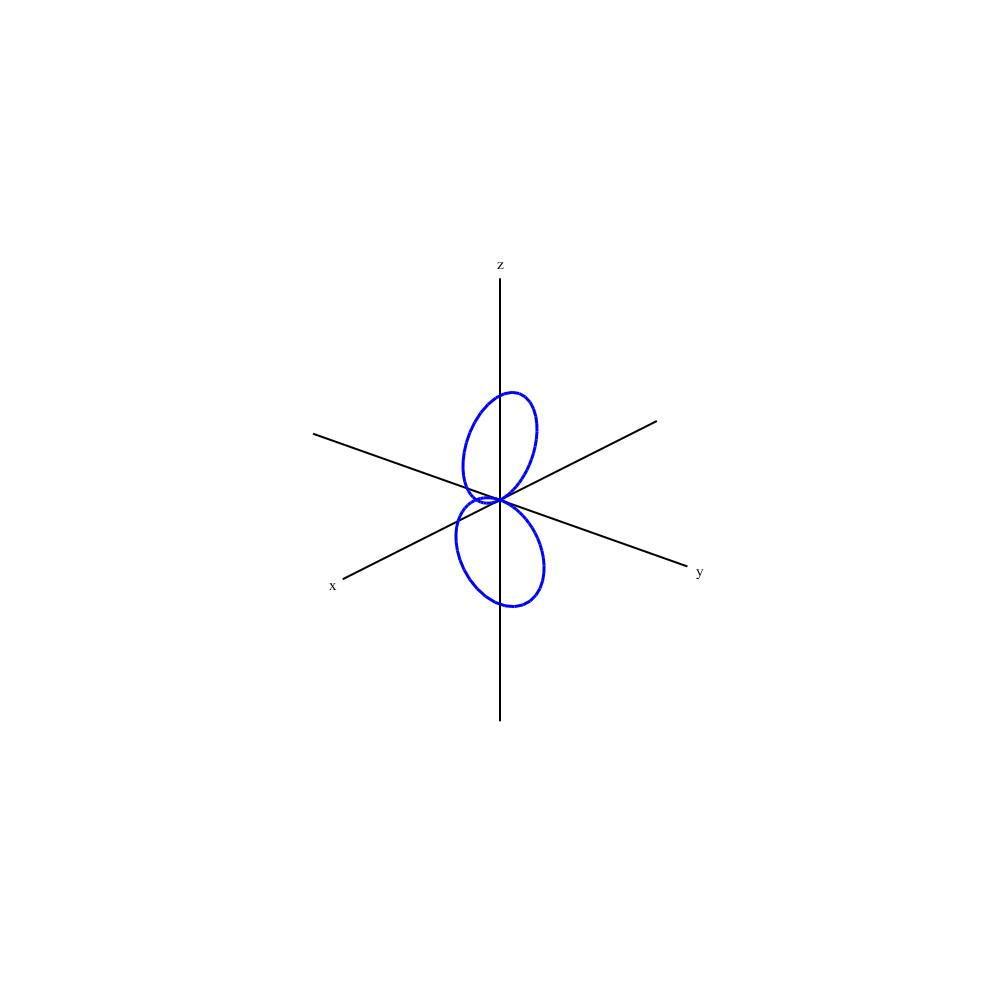
\includegraphics[scale=0.25,clip=true,
     trim=6cm 6cm 6cm 6cm]{../images/Omega[0].jpg}}%
\only<2>{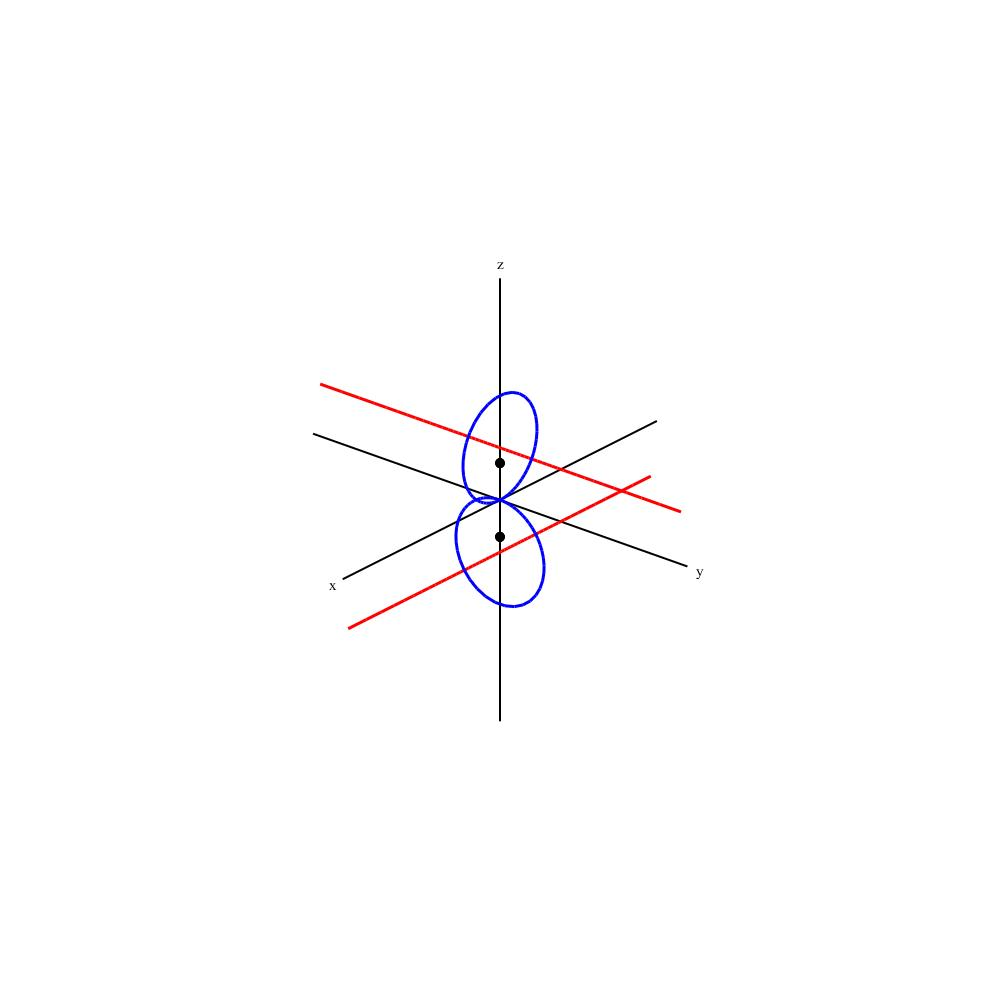
\includegraphics[scale=0.25,clip=true,
     trim=6cm 6cm 6cm 6cm]{../images/Omega[1].jpg}}%
\only<3>{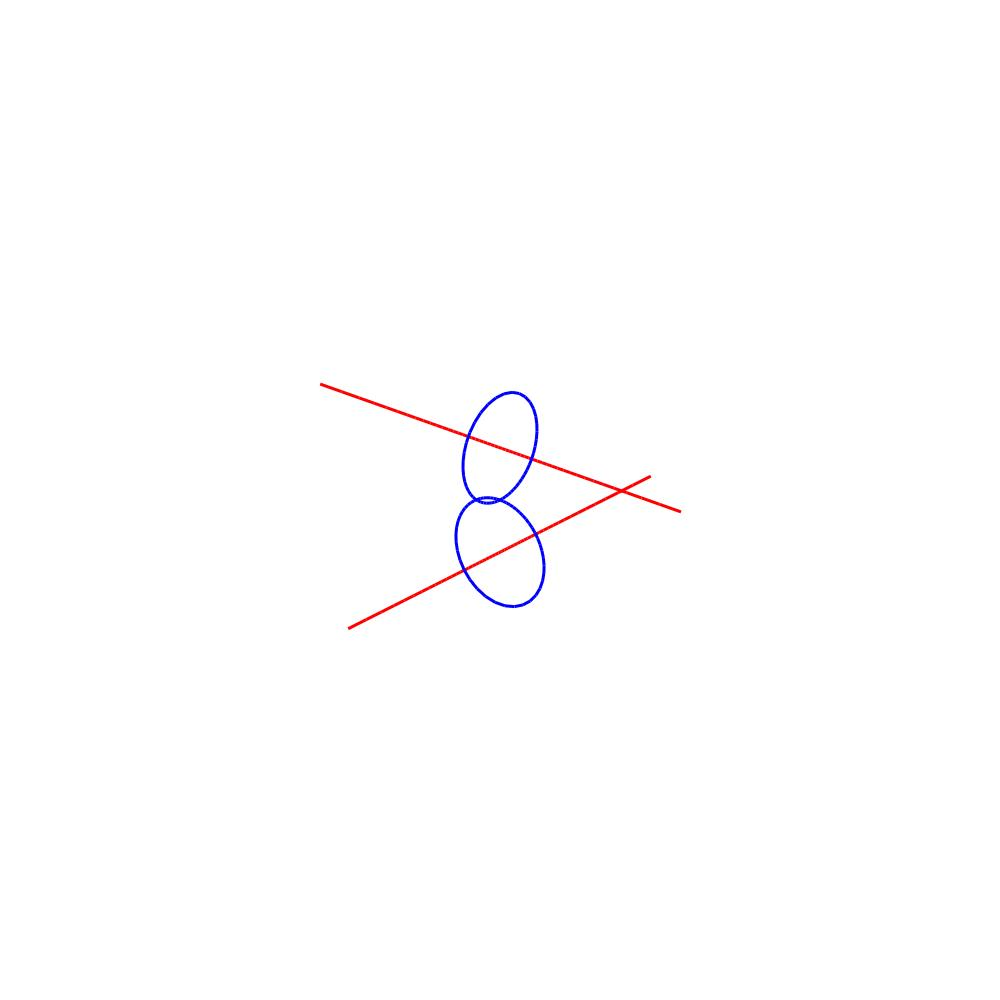
\includegraphics[scale=0.25,clip=true,
     trim=6cm 6cm 6cm 6cm]{../images/Omega[2].jpg}}%
\only<4>{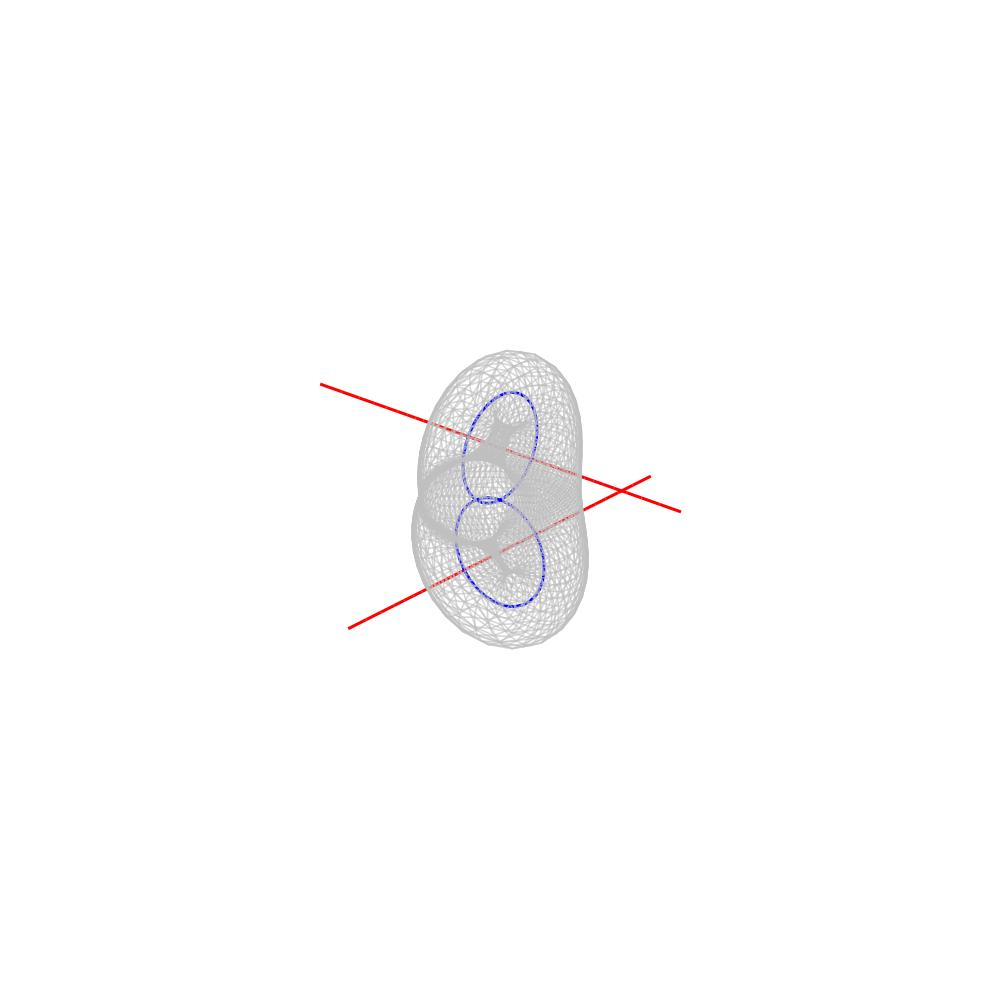
\includegraphics[scale=0.25,clip=true,
     trim=6cm 6cm 6cm 6cm]{../images/Omega[3].jpg}}%
\only<5>{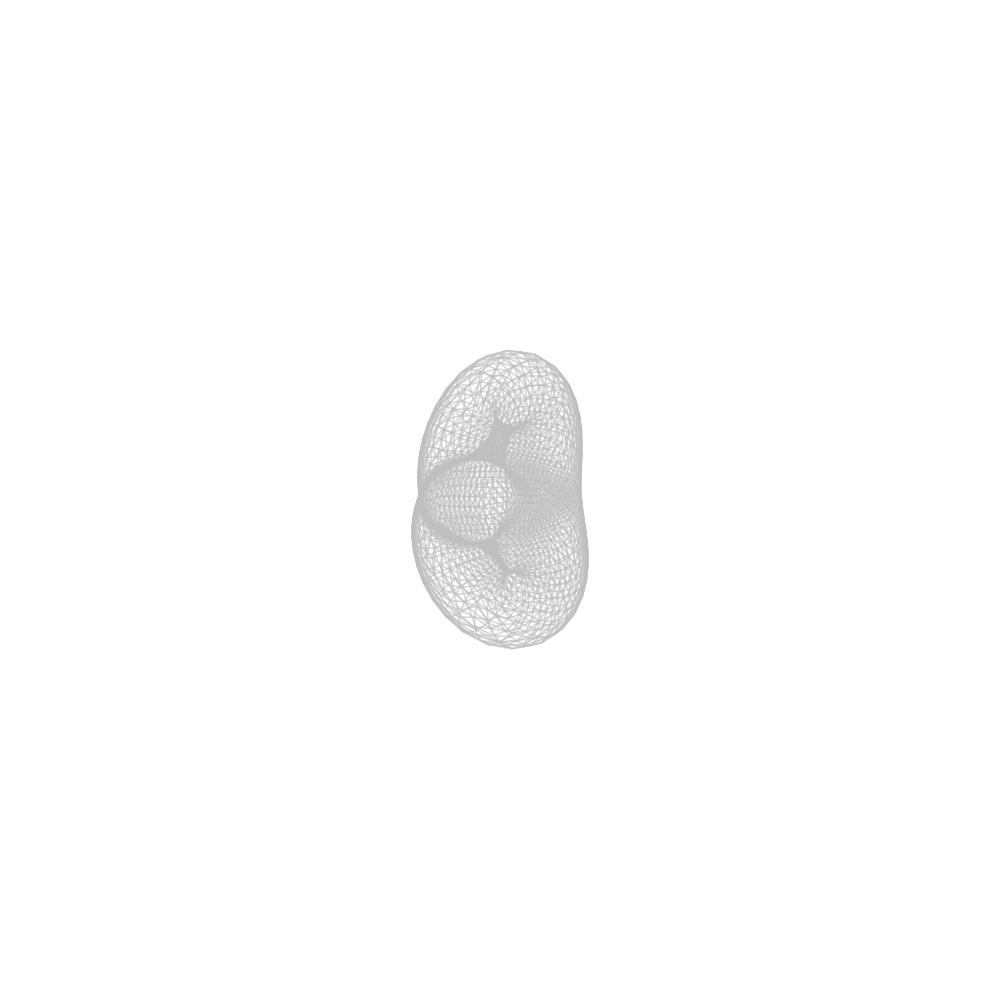
\includegraphics[scale=0.25,clip=true,
     trim=6cm 6cm 6cm 6cm]{../images/Omega[4].jpg}}%
\only<6>{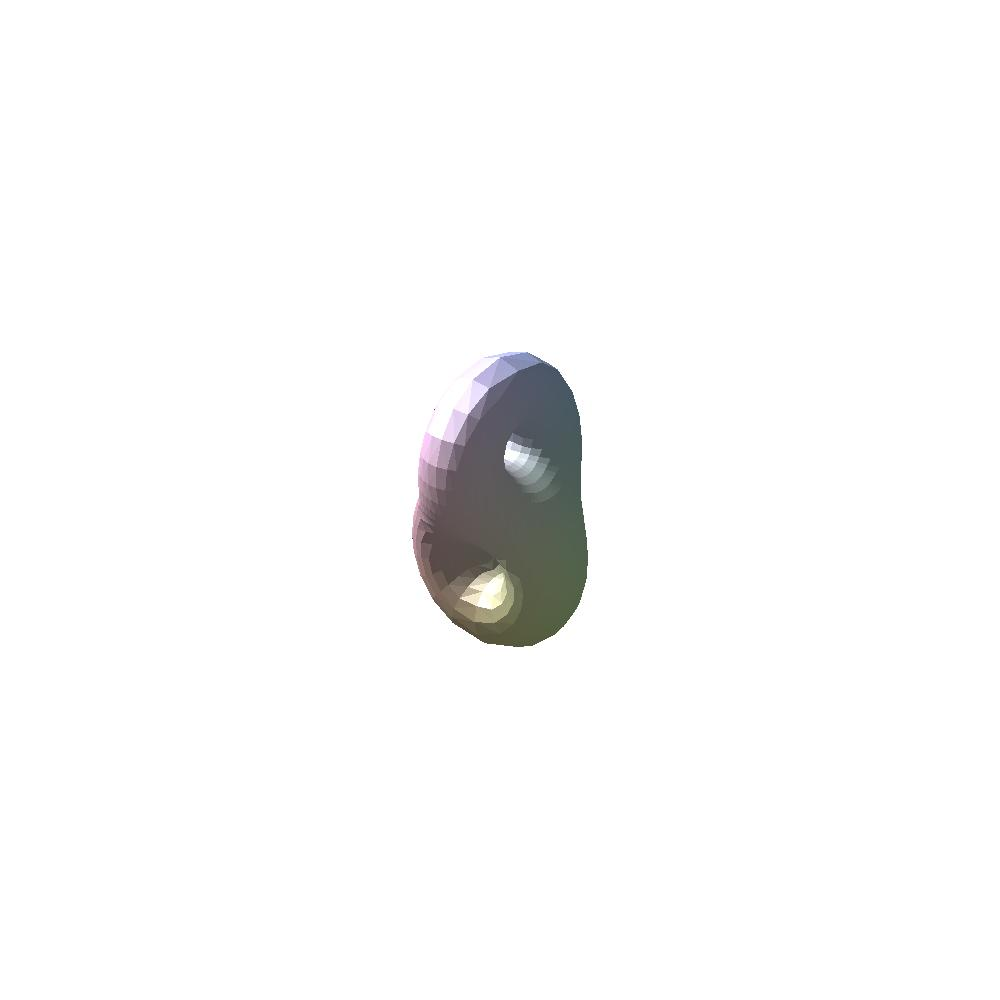
\includegraphics[scale=0.25,clip=true,
     trim=6cm 6cm 6cm 6cm]{../images/Omega[5].jpg}}%
 \]
 \begin{itemize}
  \item<1-> $f(x)=(2 x_2^2 + (x_4-1-\rt x_3)^2)(2 x_1^2 + (x_4-1+\rt x_3)^2)$; \\
   the blue set is $\{x\in S^3\st f(-x)=0\}$.
  \item<2-> The red set is $\{x\in S^3\st f(x)=0\}$.
  \item<3-> The surface is $X=\{x\in S^3\st f(x)=f(-x)\}$.
 \end{itemize}
\end{frame}

\begin{frame}[t]
 \frametitle{Cromulent surfaces}
 We define a group $G$ as follows:
 \begin{align*}
  G &= \ip{\lm,\mu,\nu\st
            \lm^4=\mu^2=\nu^2=(\mu\nu)^2=(\lm\mu)^2=(\lm\nu)^2=1} \\
    &\uc<2->{= \{\lm^i\mu^j\nu^k\st 0\leq i<4,\;0\leq j,k<2\}}
 \end{align*}
 \uc<3->{We write $V^*$ for $\{0,\dotsc,13\}$ with $G$ acting by
 \begin{align*}
  \lm &\mapsto (2\;3\;4\;5)\;(6\;7\;8\;9)\;(10\;11)\;(12\;13) \\
  \mu &\mapsto (0\;1)\;(3\;5)\;(6\;9)\;(7\;8)\;(10\;12)\;(11\;13) \\
  \nu &\mapsto (3\;5)\;(6\;9)\;(7\;8).
 \end{align*}}

 \begin{center}
  \begin{tikzpicture}[scale=1.7,auto,shorten >= 1pt]
   \uncover<4->{
    \node (v0) at ( 0, 1) [circle,draw] {$\ss 0$};
    \node (v1) at ( 0, 0) [circle,draw] {$\ss 1$};
    \node (v2) at ( 1, 1) [circle,draw] {$\ss 2$};
    \node (v3) at ( 2, 1) [circle,draw] {$\ss 3$};
    \node (v4) at ( 2, 0) [circle,draw] {$\ss 4$};
    \node (v5) at ( 1, 0) [circle,draw] {$\ss 5$};
    \node (v6) at ( 3, 1) [circle,draw] {$\ss 6$};
    \node (v7) at ( 4, 1) [circle,draw] {$\ss 7$};
    \node (v8) at ( 4, 0) [circle,draw] {$\ss 8$};
    \node (v9) at ( 3, 0) [circle,draw] {$\ss 9$};
    \node (va) at ( 5, 1) [circle,draw] {$\ss {10}$};
    \node (vb) at ( 5, 0) [circle,draw] {$\ss {11}$};
    \node (vc) at ( 6, 1) [circle,draw] {$\ss {12}$};
    \node (vd) at ( 6, 0) [circle,draw] {$\ss {13}$};
   }
   \uncover<5->{
    \draw[->,red,thick] (v2) to (v3);
    \draw[->,red,thick] (v3) to (v4);
    \draw[->,red,thick] (v4) to (v5);
    \draw[->,red,thick] (v5) to (v2);
    \draw[->,red,thick] (v6) to (v7);
    \draw[->,red,thick] (v7) to (v8);
    \draw[->,red,thick] (v8) to (v9);
    \draw[->,red,thick] (v9) to (v6);
    \draw[<->,red,thick] (va) to (vb);
    \draw[<->,red,thick] (vc) to (vd);
   }
   \uncover<6->{
    \draw[<->,olivegreen,thick] (v3) to (v5);
    \draw[<->,olivegreen,thick,bend left] (v6) to (v9);
    \draw[<->,olivegreen,thick,bend right] (v7) to (v8);
   }
   \uncover<7->{
    \draw[<->,blue,thick] (v0) to (v1);
    \draw[<->,blue,thick] (va) to (vc);
    \draw[<->,blue,thick] (vb) to (vd);
   }
  \end{tikzpicture}
 \end{center}
 \begin{center}
  \only<5>{Action of $\lm$}%
  \only<6>{Action of $\nu$}%
  \only<7>{Action of $\mu\nu$}%
 \end{center}
\end{frame}

\begin{frame}[t]
 \frametitle{Cromulent surfaces}

 {\Large\color{blue} Definition:}  A \emph{precromulent surface} is a 
 compact Riemann surface $X$ of genus 
 two with an action of $G$ such that
 \begin{itemize}
  \item[(a)] The elements $\lm$ and $\mu$ act conformally, and the element
   of $\nu$ acts anticonformally.
  \item[(b)] The set $V=\{v\in X\st \stab_{\ip{\lm,\mu}}(v)\neq 1\}$ is
   isomorphic to $V^*$ as a $G$-set.
 \end{itemize}
 \uc<2->{A \emph{precromulent labelling} of $X$ is a specific choice of
 isomorphism $V^*\simeq V$, or equivalently, a listing of the points
 in $V$ as $v_0,\dotsc,v_{13}$ such that $G$ permutes these points in
 accordance with the permutations listed on the last slide.}

 \uc<3->{
 A \emph{cromulent labelling} is a precromulent labelling such that
 \begin{itemize}
  \item[(c)] $\lm$ acts on the tangent space $T_{v_0}X$ as
   multiplication by $i$.
  \item[(d)] In the set $X'=\{x\in X\st\stab_G(x)=1\}$, there is a
   connected component $F'$ whose closure contains
   $\{v_0,v_3,v_6,v_{11}\}$.
 \end{itemize}}
 \uc<4->{One can show that every precromulent surface has precisely
 two cromulent labellings, which are exchanged by the action of
 $\lm^2$.}
 \uc<5->{A \emph{cromulent surface} is a precromulent surface with a
 choice of cromulent labelling.} 
\end{frame}

\begin{frame}[t]
 \frametitle{Cromulent}
 \[ 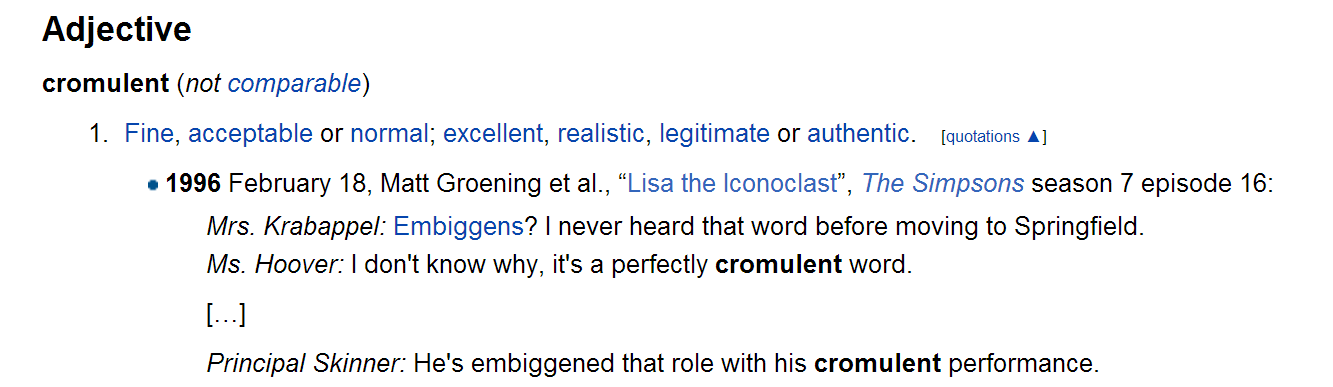
\includegraphics[scale=0.32]{../images/cromulent.png} \]
\end{frame}

\begin{frame}[t]
 \frametitle{The embedded family}
 \vspace{-1ex}
 For $a\in (0,1)$, put 
 \[ EX(a) =
    \{x\in S^3\st ((a^{-2}+1)x_3^2-2)x_4+a^{-1}(x_1^2-x_2^2)x_3=0\}.
 \]
 \uc<2->{\vspace{-5ex}
 \begin{align*}
    \lm(x_1,x_2,x_3,x_4) &= (   -x_2,\pp x_1,\pp x_3,-x_4) \\
    \mu(x_1,x_2,x_3,x_4) &= (\pp x_1,   -x_2,   -x_3,-x_4) \\
    \nu(x_1,x_2,x_3,x_4) &= (\pp x_1,   -x_2,\pp x_3,\pp x_4).
 \end{align*}}
 \vspace{-4ex}
 \uc<3->{\begin{align*}
  v_{ 0} &= (\pp 0,\pp 0,\pp 1,\pp 0) &
  v_{ 6} &= (\pp 1,\pp 1,\pp 0,\pp 0)/\rt \\
  v_{ 1} &= (\pp 0,\pp 0,   -1,\pp 0) &
  v_{ 7} &= (   -1,\pp 1,\pp 0,\pp 0)/\rt \\
  v_{ 2} &= (\pp 1,\pp 0,\pp 0,\pp 0) &
  v_{ 8} &= (   -1,   -1,\pp 0,\pp 0)/\rt \\
  v_{ 3} &= (\pp 0,\pp 1,\pp 0,\pp 0) &
  v_{ 9} &= (\pp 1,   -1,\pp 0,\pp 0)/\rt \\
  v_{ 4} &= (   -1,\pp 0,\pp 0,\pp 0) &
  v_{10} &= (0,0,\pp\rt a,\pp\sqrt{1-a^2})/\sqrt{1+a^2} \\
  v_{ 5} &= (\pp 0,-1,\pp 0,\pp 0) &
  v_{11} &= (0,0,\pp\rt a,  -\sqrt{1-a^2})/\sqrt{1+a^2} \\
  &&
  v_{12} &= (0,0,  -\rt a,  -\sqrt{1-a^2})/\sqrt{1+a^2} \\
  &&
  v_{13} &= (0,0,  -\rt a,\pp\sqrt{1-a^2})/\sqrt{1+a^2}
 \end{align*}}
 \uc<4->{Then $EX(a)$ is cromulent for all $a$, and $EX^*=EX(1/\rt)$.}  
\end{frame}

\begin{frame}[t]
 \frametitle{Special features for $a=1/\rt$}
 \begin{itemize}
  \item<2-> The complexification $CEX(a)$ is smooth for $a\neq 1/\rt$, but
   when $a=1/\rt$ it is isomorphic to Cayley's singular cubic:
   \[ X_1X_2X_3 + X_1X_2X_4 + X_1X_3X_4 + X_2X_3X_4 = 0 \]
  \item<3-> The fixed set $EX(a)^\nu$ is always a disjoint union of three
   closed curves.  If $a=1/\rt$, then one of them is a great circle.
  \item<4-> Many formulae become much simpler.
 \end{itemize}
\end{frame}


\begin{frame}[t]
 \frametitle{The projective family}
 For $a\in (0,1)$ put 
 \[ PX_0(a) = \{(w,z)\in\C^2\st w^2=z^5-(a^2+a^{-2})z^3+z\}. \]
 \uc<2->{Normalization adds a point at $\infty$ to give a smooth
 projective curve $PX(a)$.}  

 \uc<3->{Let $G$ act by
 \[
  \lm(w,z) = (iw,\;-z)      \hspace{3em}
  \mu(w,z) = (-w/z^3,\;1/z) \hspace{3em}
  \nu(w,z) = (\ov{w},\;\ov{z}).
 \]}
 \uc<4->{\begin{align*}
  v_0 &= (0,0) &
  v_1 &= \infty \\
  v_2 &= ( -(a^{-1}-a),-1) &
  v_6 &= \left(\pp \om(a^{-1}+a),\pp i\right) &
  v_{10} &= (0,-a) \\
  v_3 &= (-i(a^{-1}-a),\pp 1) &
  v_7 &= \left(-\ov{\om}(a^{-1}+a),-i\right) &
  v_{11} &= (0,\pp a) \\
  v_4 &= (\pp (a^{-1}-a),-1) &
  v_8 &= \left(-\om(a^{-1}+a),\pp i\right) &
  v_{12} &= (0,-a^{-1}) \\
  v_5 &= (\pp i(a^{-1}-a),\pp 1) &
  v_9 &= \left(\pp \ov{\om}(a^{-1}+a),-i\right) &
  v_{13} &= (0,\pp a^{-1}).
 \end{align*}
 (where $\om=e^{i\pi/4}$).}\uc<5->{  Then $PX(a)$ is cromulent.}  
\end{frame}

\begin{frame}[t]
 \frametitle{The hyperbolic family}
 Define a group $\Pi$ as follows:
 \[ \Pi = \ip{\bt_i\st i\in\Z/8}/
     \ip{\bt_i\bt_{i+4},\bt_0\bt_1\bt_2\bt_3\bt_4\bt_5\bt_6\bt_7} 
 \]
 \uc<2->{Given $a\in (0,1)$ put $a_{\pm}=\sqrt{1\pm a^2}$}\uc<3->{,\\
 and define automorphisms of $\Dl=\{z\in\C\st |z|<1\}$ by
 \begin{align*}
  \lm(z) &= iz &
  \bt_0(z) &= \frac{a_+z+1}{z+a_+} \\
  \mu(z) &= \frac{a_+z-a^2-i}{(a^2-i)z-a_+} &
  \bt_1(z) &= \frac{a_+^3z-(2+i)a^2-i}{((i-2)a^2+i)z+a_+^3} \\
  \nu(z) &= \ov{z} &
  \bt_{2n}(z) &= i^n\bt_0(z/i^n) \\
  &&
  \bt_{2n+1}(z) &= i^n\bt_1(z/i^n).
 \end{align*}}
 \uc<4->{These give an action of $\Pi$ on $\Dl$}\uc<5->{, and an action of $G$ on
 $HX(a)=\Dl/\Pi$.}  

 \uc<6->{This makes $HX(a)$ a cromulent surface.}
\end{frame}


\begin{frame}[t]
 \frametitle{Maple code}

 \begin{itemize}
  \item<2-> It is strenuous and error-prone to verify the cromulence
   axioms for $HX(a)$ by hand.  
  \item<3-> Some other verifications, to be discussed later, are even more
   strenuous.  
  \item<4-> We have instead used Maple.  The project has 30000 lines of
   Maple code, some for numerical calculation and visualization, some
   for symbolic verification.  There is a systematic framework which
   checks thousands of assertions.
  \item<5-> (By comparison, the 165 page memoir describing the project is
   generated by 15000 lines of \LaTeX.)
  \item<6-> This does not quite reach the same level of rigour as proof
   assistants like Agda or Isabelle, but it is a major step in that
   direction.
  \item<7-> All code will be released on GitHub.  
 \end{itemize}
\end{frame}

\begin{frame}[t]
 \frametitle{Universality}

 \uc<2->{{\Large\color{blue} Theorem:} For any cromulent $X$, there is a
 unique $a_P$ such that there is a (unique) cromulent isomorphism
 $X\to PX(a_P)$.}
 
 \bigskip

 \uc<3->{{\Large\color{blue} Proof:} An isotropy calculation shows that
 $X/\ip{\lm^2}$ has genus $0$, and so is isomorphic to $\C_\infty$;
 one can arrange that $v_0\mapsto 0$ and $v_1\mapsto \infty$ and
 $v_3\mapsto 1$; then the image of $v_{10}$ determines $a_P$.  \qed}

 \bigskip

 \uc<4->{{\Large\color{blue} Theorem:} For any cromulent $X$, there is a
 unique $a_H$ such that there is a (unique) cromulent isomorphism
 $HX(a_H)\to X$.}
 
 \bigskip

 \uc<5->{(Here the proof is quite intricate, but the ingredients are fairly
 standard.)}

 \bigskip

 \uc<6->{{\Large\color{blue} Conjecture:} The embedded family is also
  universal in the same sense.}

 \bigskip

 \uc<7->{{\Large\color{blue} Theorem:} We have
 $EX^*\simeq HX(a_H)\simeq PX(a_P)$, where $a_H\simeq 0.8005319$ and
 $a_P\simeq 0.0983562$.}
\end{frame}

\begin{frame}[t]
 \frametitle{Anticonformal involutions}

 \uc<2->{It is a general fact that if $X$ is a compact Riemann surface, and
 $\al\:X\to X$ is an anticonformal involution, then the fixed set
 $X^\al$ is a finite disjoint union of smoothly embedded circles.}

 \uc<3->{Thus, in a cromulent surface $X$, these sets are circles:
 \begin{align*}
  C_0 &= \text{ the component of $v_2$ in } X^{\mu\nu} \\
  C_1 &= \text{ the component of $v_0$ in } X^{\lm\nu} \\
  C_2 &= \text{ the component of $v_0$ in } X^{\lm^3\nu} \\
  C_3 &= \text{ the component of $v_{11}$ in } X^{\lm^2\nu} \\
  C_4 &= \text{ the component of $v_{10}$ in } X^\nu \\
  C_5 &= \text{ the component of $v_0$ in } X^\nu \\
  C_6 &= \text{ the component of $v_0$ in } X^{\lm^2\nu} \\
  C_7 &= \text{ the component of $v_1$ in } X^\nu \\
  C_8 &= \text{ the component of $v_1$ in } X^{\lm^2\nu}.
 \end{align*}}
\end{frame}

\begin{frame}[t]
 \frametitle{Curve systems}

 By a \emph{curve system} on a cromulent surface $X$, we mean a family
 of real analytic embeddings $c_k\:\R/2\pi\Z\to X$ (for $0\leq k\leq 8$) with values 
 {\tiny \[ \begin{array}{|c|c|c|c|c|c|c|c|c|c|c|c|c|c|c|}
   \hline
   &0&1&2&3&4&5&6&7&8&9&10&11&12&13\\ \hline
    0&&&0&\ppi&\pi&-\ppi&\tfrac{\pi}{4}&\tfrac{3\pi}{4}&-\tfrac{3\pi}{4}&-\tfrac{\pi}{4}&&&&\\ \hline
    1&0&\pi&&&&&\ppi&&-\ppi&&&&&\\ \hline
    2&0&\pi&&&&&&\ppi&&-\ppi&&&&\\ \hline
    3&&&&\ppi&&-\ppi&&&&&&0&&\pi\\ \hline
    4&&&-\ppi&&\ppi&&&&&&0&&\pi&\\ \hline
    5&0&&&&&&&&&&&\pi&&\\ \hline
    6&0&&&&&&&&&&\pi&&&\\ \hline
    7&&0&&&&&&&&&&&&\pi\\ \hline
    8&&0&&&&&&&&&&&\pi&\\ \hline
   \end{array} 
 \]}
 and equivariance
 {\tiny \begin{align*}
  \lm({\color{maplecyan}    c_{ 0}(t)}) &= {\color{maplecyan}    c_{ 0}( t+\pi/2)} &
  \mu({\color{maplecyan}    c_{ 0}(t)}) &= {\color{maplecyan}    c_{ 0}(-t)      } &
  \nu({\color{maplecyan}    c_{ 0}(t)}) &= {\color{maplecyan}    c_{ 0}(-t)      } \\      
  \lm({\color{maplegreen}   c_{ 1}(t)}) &= {\color{maplegreen}   c_{ 2}( t)      } &
  \mu({\color{maplegreen}   c_{ 1}(t)}) &= {\color{maplegreen}   c_{ 2}( t + \pi)} &
  \nu({\color{maplegreen}   c_{ 1}(t)}) &= {\color{maplegreen}   c_{ 2}(-t)      } \\      
  \lm({\color{maplegreen}   c_{ 2}(t)}) &= {\color{maplegreen}   c_{ 1}(-t)      } &
  \mu({\color{maplegreen}   c_{ 2}(t)}) &= {\color{maplegreen}   c_{ 1}( t + \pi)} &
  \nu({\color{maplegreen}   c_{ 2}(t)}) &= {\color{maplegreen}   c_{ 1}(-t)      } \\      
  \lm({\color{maplemagenta} c_{ 3}(t)}) &= {\color{maplemagenta} c_{ 4}( t)      } &
  \mu({\color{maplemagenta} c_{ 3}(t)}) &= {\color{maplemagenta} c_{ 3}( t + \pi)} &
  \nu({\color{maplemagenta} c_{ 3}(t)}) &= {\color{maplemagenta} c_{ 3}(-t)      } \\      
  \lm({\color{maplemagenta} c_{ 4}(t)}) &= {\color{maplemagenta} c_{ 3}(-t)      } &
  \mu({\color{maplemagenta} c_{ 4}(t)}) &= {\color{maplemagenta} c_{ 4}(-t - \pi)} &
  \nu({\color{maplemagenta} c_{ 4}(t)}) &= {\color{maplemagenta} c_{ 4}( t)      } \\      
  \lm({\color{mapleblue}    c_{ 5}(t)}) &= {\color{mapleblue}    c_{ 6}( t)      } &
  \mu({\color{mapleblue}    c_{ 5}(t)}) &= {\color{mapleblue}    c_{ 7}( t)      } &
  \nu({\color{mapleblue}    c_{ 5}(t)}) &= {\color{mapleblue}    c_{ 5}( t)      } \\      
  \lm({\color{mapleblue}    c_{ 6}(t)}) &= {\color{mapleblue}    c_{ 5}(-t)      } &
  \mu({\color{mapleblue}    c_{ 6}(t)}) &= {\color{mapleblue}    c_{ 8}(-t)      } &
  \nu({\color{mapleblue}    c_{ 6}(t)}) &= {\color{mapleblue}    c_{ 6}(-t)      } \\      
  \lm({\color{mapleblue}    c_{ 7}(t)}) &= {\color{mapleblue}    c_{ 8}( t)      } &
  \mu({\color{mapleblue}    c_{ 7}(t)}) &= {\color{mapleblue}    c_{ 5}( t)      } &
  \nu({\color{mapleblue}    c_{ 7}(t)}) &= {\color{mapleblue}    c_{ 7}( t)      } \\      
  \lm({\color{mapleblue}    c_{ 8}(t)}) &= {\color{mapleblue}    c_{ 7}(-t)      } &
  \mu({\color{mapleblue}    c_{ 8}(t)}) &= {\color{mapleblue}    c_{ 6}(-t)      } &
  \nu({\color{mapleblue}    c_{ 8}(t)}) &= {\color{mapleblue}    c_{ 8}(-t)      } 
 \end{align*}}
 Every cromulent surface admits a curve system, and 
 $\text{image}(c_k)=C_k$.
\end{frame}

\begin{frame}[t]
 \frametitle{A curve system for $EX^*$}
 We can define $c_0,\dotsc,c_8\:\R/2\pi\Z\to EX^*$ as follows:
 \begin{align*}
  \uc< 2->{c_0(t)} &\uc<2->{= (\cos(t),\sin(t),0,0)
                     \qquad \text{\color{blue}(a great circle)}
                   } \\
  \uc< 3->{c_1(t)} &\uc<3->{= (\sin(t)/\sqrt{2},\sin(t)/\sqrt{2},\cos(t),0)
                     \qquad \text{\color{blue}(a great circle)}
                   } \\
  \uc< 4->{c_2(t)} &\uc<4->{= \lm(c_1(t))} \\
  \uc< 5->{c_3(t)} &\uc<5->{= \left(0,\sin(t),\sqrt{2/3}\cos(t),-\sqrt{1/3}\cos(t)\right)
                    \qquad \text{\color{blue}(a great circle)}} \\
  \uc< 6->{c_4(t)} &\uc<6->{= \lm(c_3(t))} \\
  \uc< 7->{c_5(t)} &\uc<7->{= \left(-\sin(t),0,2\rt,\cos(t)-1\right)/\sqrt{10-2\cos(t)}}\\
  \uc< 8->{c_6(t)} &\uc<8->{= \lm(c_5(t))} \\
  \uc< 9->{c_7(t)} &\uc<9->{= \mu(c_5(t))} \\
  \uc<10->{c_8(t)} &\uc<10->{= \lm\mu(c_5(t))}
 \end{align*}
 \uc<11->{One can check that this gives a curve system.}
 \uc<12->{This can be generalized to cover $EX(a)$ for all $a$, but the formulae are 
 significantly more complicated.}
\end{frame}

\begin{frame}[t]
 \frametitle{A curve system for $EX^*$}

 \begin{center}
  \animategraphics[scale=0.5,autoplay,loop]{20}{../images/EXmovie/EX}{0}{89}
 \end{center}

 \begin{center}
 {\Large
 {\color{maplecyan}$c_0$}, 
 {\color{maplegreen}$c_1$}, 
 {\color{maplegreen}$c_2$}, 
 {\color{maplemagenta}$c_3$}, 
 {\color{maplemagenta}$c_4$}, 
 {\color{mapleblue}$c_5$}, 
 {\color{mapleblue}$c_6$}, 
 {\color{mapleblue}$c_7$}, 
 {\color{mapleblue}$c_8$}}
 \end{center}
\end{frame}

\begin{frame}[t]
 \frametitle{A curve system for $PX(a)$}
 Put $d(w,x,y)=(w/x^3,x/y)$; define
 $c_0,\dots,c_8\:\R/2\pi\Z\to PX(a)$ as follows:
 \begin{align*}
  c_0(t) &=
   d(-\sqrt{a^{-2}+a^2-2\cos(4t)},\;e^{it},\;e^{-it}) \\
  c_1(t) &= 
   d\left(\frac{1+i}{8\sqrt{2}}\sin(t)
           \sqrt{16\cos(t)^2+(a+a^{-1})^2\sin(t)^4},\;
           \frac{1+\cos(t)}{2},\;\frac{1-\cos(t)}{2}i\right) \\
  c_2(t) &= \lm(c_1(t)) \\
  c_3(t) &= 
   d\left(\!-i\frac{a^{-1}\!-a}{8}
               \sin(t)\sqrt{(1+a)^4-(1-a)^4\cos(t)^2}
                      \sqrt{(1+a)^2-(1-a)^2\cos(t)^2},\right. \\
         & \left.\qquad\qquad\vphantom{\frac{a^{-1}-a}{8}}
           \frac{(1+a)+(1-a)\cos(t)}{2},\;
           \frac{(1+a)-(1-a)\cos(t)}{2}\right)  \\
  c_4(t) &= \lm(c_3(t)) \\
  c_5(t) &= \left(\frac{\sin(t)}{8}\sqrt{2a(3-\cos(t))(4-a^4(1-\cos(t))^2)},\;
                    a \frac{1 - \cos(t)}{2}\right) \\
  c_6(t) &= \lm(c_5(t)),\qquad
  c_7(t)  = \mu(c_5(t)),\qquad
  c_8(t)  = \lm\mu(c_5(t)).
 \end{align*}

 \uc<2->{These give a curve system.}
\end{frame}

\begin{frame}[t]
 \frametitle{A curve system for $HX(a)$}
 
 When $|m|>1$ with $d=\sqrt{|m|^2-1}$ we have a geodesic
 $\om_m\:\R\to\Dl$:
 \[ \om_m(s) =
      \frac{id-1}{\ov{m}}
      \frac{(id+1)e^{-s} - i |m| e^s}{
            i |m| e^s + (id-1) e^{-s}}.
 \]
 \vspace{-3ex}\uc<2->{Put 
 \begin{align*}
  s_0 &= 2\log\left(\frac{\sqrt{2}a}{a_+-a_-}\right) &
  s_2 &= \log\left(\frac{1+a}{a_-}\right) &
  s_4 &= \frac{1}{4}\log\left(\frac{a_+^2+2a_++2}{a_+^2-2a_++2}\right) \\
  s_1 &= \frac{1}{2}\log\left(\frac{\sqrt{2}+a_+}{\sqrt{2}-a_+}\right) &
  s_3 &= \frac{1}{2}\log\left(\frac{a+a_++1}{a+a_+-1}\right) &
 \end{align*}}
 \uc<3->{We then define maps $\tc_k\:\R\to \Dl$ for $0\leq k\leq 8$ as follows:
 \begin{align*}
  \tc_0(t) &= \om_{(1+i)/a_+}((t/\pi-1/4)s_0) &
  \tc_5(t) &= \tanh(t\,s_3/\pi) \\
  \tc_1(t) &= e^{i\pi/4}\tanh(t\,s_1/\pi) &
  \tc_6(t) &= i\,\tanh(t\,s_3/\pi) \\
  \tc_2(t) &= e^{3i\pi/4}\tanh(t\,s_1/\pi) &
  \tc_7(t) &= \om_{ia_+/2+1/a_+}( t\,s_3/\pi - s_4) \\
  \tc_3(t) &= \om_{a_+}(-t\,s_2/\pi) &
  \tc_8(t) &= \om_{ a_+/2+i/a_+}(-t\,s_3/\pi + s_4) \\
  \tc_4(t) &= \om_{ia_+}(-t\,s_2/\pi)
 \end{align*}}
 \uc<4->{This gives a curve system on $HX(a)$.}
\end{frame}

\begin{frame}[t]
 \frametitle{Pictures for $HX(a)$}
 \vspace{-4ex}
 \begin{center}
  \only<1>{\begin{tikzpicture}[scale=3.5]
  \draw (0,0) circle(1);
  \draw[blue] (-1,0) -- (1,0);
  \draw[blue] (0,-1) -- (0,1);
  \draw[green] (-0.707,-0.707) -- ( 0.707, 0.707);
  \draw[green] (-0.707, 0.707) -- ( 0.707,-0.707);
  \draw[cyan] (0.800,0.800) (0.294,0.956) arc(-197:-73:0.529);
  \draw[cyan,dotted] (-0.800,0.800) (-0.956,0.294) arc(-107:17:0.529);
  \draw[cyan,dotted] (-0.800,-0.800) (-0.294,-0.956) arc(-17:107:0.529);
  \draw[cyan,dotted] (0.800,-0.800) (0.956,-0.294) arc(73:197:0.529);
  \draw[magenta] (1.250,0.000) (0.800,0.600) arc(127:233:0.750);
  \draw[magenta,dotted] (0.000,1.250) (-0.600,0.800) arc(-143:-37:0.750);
  \draw[magenta,dotted] (-1.250,0.000) (-0.800,-0.600) arc(-53:53:0.750);
  \draw[magenta,dotted] (0.000,-1.250) (0.600,-0.800) arc(37:143:0.750);
  \draw[magenta] (0.000,1.250) (-0.600,0.800) arc(-143:-37:0.750);
  \draw[magenta,dotted] (-1.250,0.000) (-0.800,-0.600) arc(-53:53:0.750);
  \draw[magenta,dotted] (0.000,-1.250) (0.600,-0.800) arc(37:143:0.750);
  \draw[magenta,dotted] (1.250,0.000) (0.800,0.600) arc(127:233:0.750);
  \draw[blue] (0.800,0.625) (0.670,0.742) arc(-222:-62:0.175);
  \draw[blue,dotted] (-0.625,0.800) (-0.742,0.670) arc(-132:28:0.175);
  \draw[blue,dotted] (-0.800,-0.625) (-0.670,-0.742) arc(-42:118:0.175);
  \draw[blue,dotted] (0.625,-0.800) (0.742,-0.670) arc(48:208:0.175);
  \draw[blue] (0.625,0.800) (0.471,0.882) arc(-208:-48:0.175);
  \draw[blue,dotted] (-0.800,0.625) (-0.882,0.471) arc(-118:42:0.175);
  \draw[blue,dotted] (-0.625,-0.800) (-0.471,-0.882) arc(-28:132:0.175);
  \draw[blue,dotted] (0.800,-0.625) (0.882,-0.471) arc(62:222:0.175);
  \fill[black](0.000,0.000) circle(0.007);
  \fill[black](0.625,0.625) circle(0.007);
  \fill[black](0.322,0.573) circle(0.007);
  \fill[black](-0.573,0.322) circle(0.007);
  \fill[black](-0.322,-0.573) circle(0.007);
  \fill[black](0.573,-0.322) circle(0.007);
  \fill[black](0.426,0.426) circle(0.007);
  \fill[black](-0.426,0.426) circle(0.007);
  \fill[black](-0.426,-0.426) circle(0.007);
  \fill[black](0.426,-0.426) circle(0.007);
  \fill[black](0.000,0.500) circle(0.007);
  \fill[black](0.500,0.000) circle(0.007);
  \fill[gray!60](-0.500,0.000) circle(0.007);
  \fill[black](-0.493,0.685) circle(0.007);
  \fill[black](0.685,0.493) circle(0.007);
  \fill[gray!60](-0.625,-0.625) circle(0.007);
  \fill[gray!60](-0.322,0.573) circle(0.007);
  \fill[gray!60](-0.625,0.625) circle(0.007);
  \fill[gray!60](0.000,-0.500) circle(0.007);
  \fill[gray!60](0.493,0.685) circle(0.007);
  \fill[gray!60](0.625,-0.625) circle(0.007);
  \fill[gray!60](-0.573,-0.322) circle(0.007);
  \fill[gray!60](0.685,-0.493) circle(0.007);
  \fill[gray!60](0.493,-0.685) circle(0.007);
  \fill[gray!60](-0.685,-0.493) circle(0.007);
  \fill[gray!60](0.322,-0.573) circle(0.007);
  \fill[gray!60](-0.493,-0.685) circle(0.007);
  \fill[gray!60](-0.685,0.493) circle(0.007);
  \fill[gray!60](0.573,0.322) circle(0.007);
  \draw( 0.30, 0.25) node{$\sss c_1$};
  \draw(-0.30, 0.25) node{$\sss c_2$};
  \draw( 0.80,-0.03) node{$\sss c_5$};
  \draw(-0.05, 0.80) node{$\sss c_6$};
  \draw( 0.773, 0.246) node{$\sss c_{0}$};
  \draw( 0.486, 0.179) node{$\sss c_{3}$};
  \draw(-0.229, 0.566) node{$\sss c_{4}$};
  \draw( 0.771, 0.422) node{$\sss c_{7}$};
  \draw( 0.422, 0.771) node{$\sss c_{8}$};
  \draw( 0.060, 0.020) node{$\sss v_{0}$};
  \draw( 0.655, 0.595) node{$\sss v_{1}$};
  \draw( 0.272, 0.583) node{$\sss v_{2}$};
  \draw(-0.623, 0.322) node{$\sss v_{3.1}$};
  \draw(-0.372,-0.573) node{$\sss v_{4.1}$};
  \draw( 0.623,-0.322) node{$\sss v_{5}$};
  \draw( 0.386, 0.426) node{$\sss v_{6}$};
  \draw(-0.386, 0.426) node{$\sss v_{7}$};
  \draw(-0.396,-0.456) node{$\sss v_{8}$};
  \draw( 0.396,-0.456) node{$\sss v_{9}$};
  \draw(-0.040, 0.470) node{$\sss v_{10}$};
  \draw( 0.470,-0.030) node{$\sss v_{11}$};
  \draw(-0.440,-0.030) node{$\sss v_{11.1}$};
  \draw( 0.443, 0.685) node{$\sss v_{12}$};
  \draw( 0.635, 0.493) node{$\sss v_{13}$};
  \draw(-0.655,-0.595) node{$\sss v_{1.2}$};
  \draw(-0.382, 0.573) node{$\sss v_{4}$};
  \draw(-0.675, 0.595) node{$\sss v_{1.1}$};
  \draw(-0.060,-0.530) node{$\sss v_{10.1}$};
  \draw(-0.433, 0.685) node{$\sss v_{12.2}$};
  \draw( 0.655,-0.595) node{$\sss v_{1.3}$};
  \draw(-0.623,-0.322) node{$\sss v_{5.1}$};
  \draw( 0.745,-0.493) node{$\sss v_{13.2}$};
  \draw(-0.433,-0.685) node{$\sss v_{12.1}$};
  \draw(-0.745,-0.493) node{$\sss v_{13.1}$};
  \draw( 0.382,-0.563) node{$\sss v_{2.1}$};
  \draw( 0.433,-0.685) node{$\sss v_{12.3}$};
  \draw(-0.745, 0.493) node{$\sss v_{13.3}$};
  \draw( 0.523, 0.312) node{$\sss v_{3}$};
  \end{tikzpicture}}\only<2>{
  \begin{tikzpicture}[scale=3.5]
  \draw[magenta]( 1.250, 0.000) +(139:0.750) arc(139:221:0.750);
  \draw[blue]   ( 0.800, 0.625) +(180:0.175) arc(180:229:0.175);
  \draw[blue]   ( 0.625, 0.800) +(221:0.175) arc(221:270:0.175);
  \draw[magenta]( 0.000, 1.250) +(229:0.750) arc(229:311:0.750);
  \draw[blue]   (-0.625, 0.800) +(270:0.175) arc(270:319:0.175);
  \draw[blue]   (-0.800, 0.625) +(311:0.175) arc(311:360:0.175);
  \draw[magenta](-1.250, 0.000) +(-41:0.750) arc(-41: 41:0.750);
  \draw[blue]   (-0.800,-0.625) +(  0:0.175) arc(  0: 49:0.175);
  \draw[blue]   (-0.625,-0.800) +( 41:0.175) arc( 41: 90:0.175);
  \draw[magenta]( 0.000,-1.250) +( 49:0.750) arc( 49:131:0.750);
  \draw[blue]   ( 0.625,-0.800) +( 90:0.175) arc( 90:139:0.175);
  \draw[blue]   ( 0.800,-0.625) +(131:0.175) arc(131:180:0.175);
  \draw[magenta,->] ( 0.500, 0.000) -- ( 0.500,-0.001);
  \draw[magenta,->] (-0.500, 0.000) -- (-0.500,-0.001);
  \draw[magenta,->] ( 0.000, 0.500) -- (-0.001, 0.500);
  \draw[magenta,->] ( 0.000,-0.500) -- (-0.001,-0.500);
  \draw[blue,->] ( 0.800, 0.625) +(205:0.175) -- +(206:0.175);
  \draw[blue,->] ( 0.625, 0.800) +(246:0.175) -- +(245:0.175);
  \draw[blue,->] (-0.625, 0.800) +(295:0.175) -- +(296:0.175);
  \draw[blue,->] (-0.800, 0.625) +(335:0.175) -- +(334:0.175);
  \draw[blue,->] (-0.800,-0.625) +( 25:0.175) -- +( 26:0.175);
  \draw[blue,->] (-0.625,-0.800) +( 65:0.175) -- +( 64:0.175);
  \draw[blue,->] ( 0.625,-0.800) +(115:0.175) -- +(116:0.175);
  \draw[blue,->] ( 0.800,-0.625) +(155:0.175) -- +(154:0.175);
  \fill( 0.685, 0.493) circle(0.01);
  \fill( 0.625, 0.625) circle(0.01);
  \fill( 0.493, 0.685) circle(0.01);
  \fill(-0.493, 0.685) circle(0.01);
  \fill(-0.625, 0.625) circle(0.01);
  \fill(-0.685, 0.493) circle(0.01);
  \fill(-0.685,-0.493) circle(0.01);
  \fill(-0.625,-0.625) circle(0.01);
  \fill(-0.493,-0.685) circle(0.01);
  \fill( 0.493,-0.685) circle(0.01);
  \fill( 0.625,-0.625) circle(0.01);
  \fill( 0.685,-0.493) circle(0.01);
  \draw( 0.685, 0.493) node[anchor=west]{$\sss v_{13}$};
  \draw( 0.625, 0.625) node[anchor=south west]{$\sss v_{1}$};
  \draw( 0.493, 0.685) node[anchor=south]{$\sss v_{12}$};
  \draw(-0.493, 0.685) node[anchor=south]{$\sss v_{12.2}$};
  \draw(-0.625, 0.625) node[anchor=south east]{$\sss v_{1.1}$};
  \draw(-0.685, 0.493) node[anchor=east]{$\sss v_{13.3}$};
  \draw(-0.685,-0.493) node[anchor=east]{$\sss v_{13.1}$};
  \draw(-0.625,-0.625) node[anchor=north east]{$\sss v_{1.2}$};
  \draw(-0.493,-0.685) node[anchor=north]{$\sss v_{12.1}$};
  \draw( 0.493,-0.685) node[anchor=north]{$\sss v_{12.3}$};
  \draw( 0.625,-0.625) node[anchor=north west]{$\sss v_{1.3}$};
  \draw( 0.685,-0.493) node[anchor=west]{$\sss v_{13.2}$};
  \draw( 0.535, 0.605) node{$\sss a$};
  \draw(-0.530, 0.605) node{$\sss *a$};
  \draw( 0.000, 0.450) node{$\sss b$};
  \draw( 0.000,-0.450) node{$\sss *b$};
  \draw(-0.595, 0.532) node{$\sss c$};
  \draw(-0.590,-0.532) node{$\sss *c$};
  \draw(-0.450, 0.000) node{$\sss d$};
  \draw( 0.445, 0.000) node{$\sss *d$};
  \draw(-0.535,-0.605) node{$\sss e$};
  \draw( 0.539,-0.605) node{$\sss *e$};
  \draw( 0.595,-0.532) node{$\sss f$};
  \draw( 0.590, 0.532) node{$\sss *f$};
  \end{tikzpicture}}
 \end{center}
\end{frame}

\begin{frame}[t]
 \frametitle{Fundamental domains and nets}
\begin{center}
 {\tiny \begin{tikzpicture}[scale=.25]
  \draw[  green] (  0,  0) -- (  6,  6);
  \draw[  green] (  0,  0) -- ( -6,  6);
  \draw[  green] (  0,  0) -- ( -6, -6);
  \draw[  green] (  0,  0) -- (  6, -6);
  \draw[   blue] (  0,  0) -- (  0,  8);
  \draw[   blue] (  0,  0) -- (  0, -8);
  \draw[   blue] (  0,  0) -- (  8,  0);
  \draw[   blue] (  0,  0) -- ( -8,  0);
  \draw[   blue] ( 12, 12) -- (  4, 12);
  \draw[   blue] ( 12, 12) -- ( 12,  4);
  \draw[  green] ( 12, 12) -- (  6,  6);
  \draw[  green] (-12, 12) -- ( -6,  6);
  \draw[  green] (-12,-12) -- ( -6, -6);
  \draw[  green] ( 12,-12) -- (  6, -6);
  \draw[   cyan] (  4,  8) -- (  6,  6);
  \draw[magenta] (  4,  8) -- (  0,  8);
  \draw[magenta] (  4,  8) -- (  4, 12);
  \draw[   cyan] (  8,  4) -- (  6,  6);
  \draw[magenta] (  8,  4) -- (  8,  0);
  \draw[magenta] (  8,  4) -- ( 12,  4);
  \draw[   cyan] ( -4,  8) -- ( -6,  6);
  \draw[magenta] ( -4,  8) -- (  0,  8);
  \draw[magenta] ( -4,  8) -- ( -4, 12);
  \draw[   cyan] (  8, -4) -- (  6, -6);
  \draw[magenta] (  8, -4) -- (  8,  0);
  \draw[magenta] (  8, -4) -- ( 12, -4);
  \draw[   blue] (-12, 12) -- ( -4, 12);
  \draw[   blue] (-12, 12) -- (-12,  4);
  \draw[   blue] (-12,-12) -- ( -4,-12);
  \draw[   blue] (-12,-12) -- (-12, -4);
  \draw[   blue] ( 12,-12) -- (  4,-12);
  \draw[   blue] ( 12,-12) -- ( 12, -4);
  \draw[   cyan] (  4, -8) -- (  6, -6);
  \draw[magenta] (  4, -8) -- (  0, -8);
  \draw[magenta] (  4, -8) -- (  4,-12);
  \draw[   cyan] ( -8,  4) -- ( -6,  6);
  \draw[magenta] ( -8,  4) -- ( -8,  0);
  \draw[magenta] ( -8,  4) -- (-12,  4);
  \draw[   cyan] ( -4, -8) -- ( -6, -6);
  \draw[magenta] ( -4, -8) -- (  0, -8);
  \draw[magenta] ( -4, -8) -- ( -4,-12);
  \draw[   cyan] ( -8, -4) -- ( -6, -6);
  \draw[magenta] ( -8, -4) -- ( -8,  0);
  \draw[magenta] ( -8, -4) -- (-12, -4);
  \draw[-angle 90, cyan] (  4,  8) -- (  5,  7);
  \draw[-angle 90, cyan] (  6,  6) -- (  7,  5);
  \draw[-angle 90, cyan] (  8, -4) -- (  7, -5);
  \draw[-angle 90, cyan] (  6, -6) -- (  5, -7);
  \draw[-angle 90, cyan] ( -4, -8) -- ( -5, -7);
  \draw[-angle 90, cyan] ( -6, -6) -- ( -7, -5);
  \draw[-angle 90, cyan] ( -8,  4) -- ( -7,  5);
  \draw[-angle 90, cyan] ( -6,  6) -- ( -5,  7);
  \draw ( -5,  7) node[anchor=north west] {$\ss c_0$};
  \draw (  5,  7) node[anchor=north east] {$\ss c_0$};
  \draw ( -5, -7) node[anchor=south west] {$\ss c_0$};
  \draw (  5, -7) node[anchor=south east] {$\ss c_0$};
  \draw[-angle 90,green] (  3,  3) -- (  4,  4);
  \draw[-angle 90,green] (  7,  7) -- (  8,  8);
  \draw[-angle 90,green] ( -5, -5) -- ( -4, -4);
  \draw[-angle 90,green] ( -9, -9) -- ( -8, -8);
  \draw (  4,  4) node[anchor=north west] {$\ss c_1$};
  \draw[-angle 90,green] ( -3,  3) -- ( -4,  4);
  \draw[-angle 90,green] ( -7,  7) -- ( -8,  8);
  \draw[-angle 90,green] (  5, -5) -- (  4, -4);
  \draw[-angle 90,green] (  9, -9) -- (  8, -8);
  \draw ( -4,  4) node[anchor=north east] {$\ss c_2$};
  \draw[-angle 90,magenta] (-11, -4) -- (-10, -4);
  \draw[-angle 90,magenta] ( -8, -4) -- ( -8, -2);
  \draw[-angle 90,magenta] ( -8,  0) -- ( -8,  2);
  \draw[-angle 90,magenta] ( -9,  4) -- (-10,  4);
  \draw ( -8, -2) node[anchor=east] {$\ss c_3$};
  \draw[-angle 90,magenta] ( 11, -4) -- ( 10, -4);
  \draw[-angle 90,magenta] (  8, -4) -- (  8, -2);
  \draw[-angle 90,magenta] (  8,  0) -- (  8,  2);
  \draw[-angle 90,magenta] (  9,  4) -- ( 10,  4);
  \draw (  8, -2) node[anchor=west] {$\ss c_3$};
  \draw[-angle 90,magenta] (  4, 11) -- (  4, 10);
  \draw[-angle 90,magenta] (  4,  8) -- (  2,  8);
  \draw[-angle 90,magenta] (  0,  8) -- ( -2,  8);
  \draw[-angle 90,magenta] ( -4,  9) -- ( -4, 10);
  \draw ( -2,  8) node[anchor=south] {$\ss c_4$};
  \draw[-angle 90,magenta] (  4,-11) -- (  4,-10);
  \draw[-angle 90,magenta] (  4, -8) -- (  2, -8);
  \draw[-angle 90,magenta] (  0, -8) -- ( -2, -8);
  \draw[-angle 90,magenta] ( -4, -9) -- ( -4,-10);
  \draw ( -2, -8) node[anchor=north] {$\ss c_4$};
  \draw[-angle 90,blue] (  3,  0) -- (  4,  0);
  \draw[-angle 90,blue] ( -5,  0) -- ( -4,  0);
  \draw (  4,  0) node[anchor=north] {$\ss c_5$};
  \draw[-angle 90,blue] (  0,  3) -- (  0,  4);
  \draw[-angle 90,blue] (  0, -5) -- (  0, -4);
  \draw (  0,  4) node[anchor=east] {$\ss c_6$};
  \draw[-angle 90,blue] (-12,  7) -- (-12,  8);
  \draw[-angle 90,blue] (-12, -7) -- (-12, -8);
  \draw[-angle 90,blue] ( 12,  9) -- ( 12,  8);
  \draw[-angle 90,blue] ( 12, -9) -- ( 12, -8);
  \draw (-12,  8) node[anchor=east] {$\ss c_7$};
  \draw (-12, -8) node[anchor=east] {$\ss c_7$};
  \draw ( 12,  8) node[anchor=west] {$\ss c_7$};
  \draw ( 12, -8) node[anchor=west] {$\ss c_7$};
  \draw[-angle 90,blue] ( -9, 12) -- ( -8, 12);
  \draw[-angle 90,blue] (  9, 12) -- (  8, 12);
  \draw[-angle 90,blue] ( -7,-12) -- ( -8,-12);
  \draw[-angle 90,blue] (  7,-12) -- (  8,-12);
  \draw (  8,-12) node[anchor=north] {$\ss c_8$};
  \draw ( -8,-12) node[anchor=north] {$\ss c_8$};
  \draw (  8, 12) node[anchor=south] {$\ss c_8$};
  \draw ( -8, 12) node[anchor=south] {$\ss c_8$};
  \fill[black] (  0,  0) circle(0.10);
  \fill[black] ( -4, -8) circle(0.10);
  \fill[black] ( 12, 12) circle(0.10);
  \fill[black] (  4,  8) circle(0.10);
  \fill[black] (  8,  4) circle(0.10);
  \fill[black] ( -4,  8) circle(0.10);
  \fill[black] (  8, -4) circle(0.10);
  \fill[black] (  6,  6) circle(0.10);
  \fill[black] ( -6,  6) circle(0.10);
  \fill[black] (  6, -6) circle(0.10);
  \fill[black] ( -6, -6) circle(0.10);
  \fill[black] (  8,  0) circle(0.10);
  \fill[black] (  0,  8) circle(0.10);
  \fill[black] ( 12,  4) circle(0.10);
  \fill[black] (  4, 12) circle(0.10);
  \fill[black] ( -8,  4) circle(0.10);
  \fill[black] (  0, -8) circle(0.10);
  \fill[black] ( -8, -4) circle(0.10);
  \fill[black] (-12,  4) circle(0.10);
  \fill[black] ( -4,-12) circle(0.10);
  \fill[black] (-12, 12) circle(0.10);
  \fill[black] (-12,-12) circle(0.10);
  \fill[black] ( -8,  0) circle(0.10);
  \fill[black] (-12, -4) circle(0.10);
  \fill[black] (  4,-12) circle(0.10);
  \fill[black] ( 12,-12) circle(0.10);
  \fill[black] ( 12, -4) circle(0.10);
  \fill[black] (  4, -8) circle(0.10);
  \fill[black] ( -4, 12) circle(0.10);
  \draw (  0,  0) node[anchor=north]{$\ss v_{0}$};
  \draw ( -4, -8) node[anchor=north west]{$\ss v_{4.1}$};
  \draw ( 12, 12) node[anchor=south west]{$\ss v_{1}$};
  \draw (  4,  8) node[anchor=south east]{$\ss v_{2}$};
  \draw (  8,  4) node[anchor=north west]{$\ss v_{3}$};
  \draw ( -4,  8) node[anchor=south west]{$\ss v_{4}$};
  \draw (  8, -4) node[anchor=south west]{$\ss v_{5}$};
  \draw (  6,  6) node[anchor=north]{$\ss v_{6}$};
  \draw ( -6,  6) node[anchor=north]{$\ss v_{7}$};
  \draw (  6, -6) node[anchor=north]{$\ss v_{9}$};
  \draw ( -6, -6) node[anchor=north]{$\ss v_{8}$};
  \draw (  8,  0) node[anchor=west]{$\ss v_{11}$};
  \draw (  0,  8) node[anchor=south]{$\ss v_{10}$};
  \draw ( 12,  4) node[anchor=north west]{$\ss v_{13}$};
  \draw (  4, 12) node[anchor=south east]{$\ss v_{12}$};
  \draw ( -8,  4) node[anchor=north east]{$\ss v_{3.1}$};
  \draw (  0, -8) node[anchor=north]{$\ss v_{10.1}$};
  \draw ( -8, -4) node[anchor=south east]{$\ss v_{5.1}$};
  \draw (-12,  4) node[anchor=north east]{$\ss v_{13.3}$};
  \draw ( -4,-12) node[anchor=north west]{$\ss v_{12.1}$};
  \draw (-12, 12) node[anchor=south east]{$\ss v_{1.1}$};
  \draw (-12,-12) node[anchor=north east]{$\ss v_{1.2}$};
  \draw ( -8,  0) node[anchor=east]{$\ss v_{11.1}$};
  \draw (-12, -4) node[anchor=south east]{$\ss v_{13.1}$};
  \draw (  4,-12) node[anchor=north east]{$\ss v_{12.3}$};
  \draw ( 12,-12) node[anchor=north west]{$\ss v_{1.3}$};
  \draw ( 12, -4) node[anchor=south west]{$\ss v_{13.2}$};
  \draw (  4, -8) node[anchor=north east]{$\ss v_{2.1}$};
  \draw ( -4, 12) node[anchor=south west]{$\ss v_{12.2}$};
  \draw (6.00,2.00) node{$1$};
  \draw (-2.00,6.00) node{$\lm$};
  \draw (-6.00,-2.00) node{$\lm^2$};
  \draw (2.00,-6.00) node{$\lm^3$};
  \draw (10.00,-6.00) node{$\mu$};
  \draw (6.00,10.00) node{$\lm\mu$};
  \draw (-10.00,6.00) node{$\lm^2\mu$};
  \draw (-6.00,-10.00) node{$\lm^3\mu$};
  \draw (6.00,-2.00) node{$\nu$};
  \draw (2.00,6.00) node{$\lm\nu$};
  \draw (-6.00,2.00) node{$\lm^2\nu$};
  \draw (-2.00,-6.00) node{$\lm^3\nu$};
  \draw (10.00,6.00) node{$\mu\nu$};
  \draw (-6.00,10.00) node{$\lm\mu\nu$};
  \draw (-10.00,-6.00) node{$\lm^2\mu\nu$};
  \draw (6.00,-10.00) node{$\lm^3\mu\nu$};
 \end{tikzpicture}}
\end{center}
Any cromulent surface has a net as shown above.  Each of the 16
regions is a fundamental domain for the action of $G$. 
\end{frame}

\begin{frame}[t]
 \frametitle{Alternative nets}

 \only<2>{\tiny\begin{center}
  \begin{tikzpicture}[scale=0.8]
   \draw[  green] (  4,  4) -- (  3,  3);
   \draw[   blue] (  4,  4) -- (  0,  4);
   \draw[   blue] (  4,  4) -- (  4,  0);
   \draw[  green] (  2,  2) -- (  3,  3);
   \draw[   blue] (  2,  2) -- (  0,  2);
   \draw[   blue] (  2,  2) -- (  2,  0);
   \draw[   cyan] (  0,  3) -- ( -3,  3);
   \draw[   cyan] (  0,  3) -- (  3,  3);
   \draw[magenta] (  0,  3) -- (  0,  4);
   \draw[magenta] (  0,  3) -- (  0,  2);
   \draw[   cyan] ( -3,  0) -- ( -3,  3);
   \draw[   cyan] ( -3,  0) -- ( -3, -3);
   \draw[magenta] ( -3,  0) -- ( -4,  0);
   \draw[magenta] ( -3,  0) -- ( -2,  0);
   \draw[   cyan] (  0, -3) -- ( -3, -3);
   \draw[   cyan] (  0, -3) -- (  3, -3);
   \draw[magenta] (  0, -3) -- (  0, -4);
   \draw[magenta] (  0, -3) -- (  0, -2);
   \draw[   cyan] (  3,  0) -- (  3, -3);
   \draw[   cyan] (  3,  0) -- (  3,  3);
   \draw[magenta] (  3,  0) -- (  4,  0);
   \draw[magenta] (  3,  0) -- (  2,  0);
   \draw[  green] ( -4,  4) -- ( -3,  3);
   \draw[   blue] ( -4,  4) -- (  0,  4);
   \draw[   blue] ( -4,  4) -- ( -4,  0);
   \draw[  green] ( -4, -4) -- ( -3, -3);
   \draw[   blue] ( -4, -4) -- (  0, -4);
   \draw[   blue] ( -4, -4) -- ( -4,  0);
   \draw[  green] (  4, -4) -- (  3, -3);
   \draw[   blue] (  4, -4) -- (  4,  0);
   \draw[   blue] (  4, -4) -- (  0, -4);
   \draw[  green] ( -2,  2) -- ( -3,  3);
   \draw[   blue] ( -2,  2) -- (  0,  2);
   \draw[   blue] ( -2,  2) -- ( -2,  0);
   \draw[  green] ( -2, -2) -- ( -3, -3);
   \draw[   blue] ( -2, -2) -- (  0, -2);
   \draw[   blue] ( -2, -2) -- ( -2,  0);
   \draw[  green] (  2, -2) -- (  3, -3);
   \draw[   blue] (  2, -2) -- (  2,  0);
   \draw[   blue] (  2, -2) -- (  0, -2);
   \draw (  4,  4) node[anchor=south west]{$\ss 0$};
   \draw (  2,  2) node[anchor=north east]{$\ss 1$};
   \draw (  0,  3) node{$\ss 2$};
   \draw ( -3,  0) node{$\ss 3$};
   \draw (  0, -3) node{$\ss 4$};
   \draw (  3,  0) node{$\ss 5$};
   \draw ( -3,  3) node{$\ss 6$};
   \draw ( -3, -3) node{$\ss 7$};
   \draw (  3,  3) node{$\ss 9$};
   \draw (  3, -3) node{$\ss 8$};
   \draw (  4,  0) node[anchor=west]{$\ss 11$};
   \draw (  0,  4) node[anchor=south]{$\ss 10$};
   \draw (  2,  0) node[anchor=east]{$\ss 13$};
   \draw (  0,  2) node[anchor=north]{$\ss 12$};
   \draw (  0, -4) node[anchor=north]{$\ss 10.1$};
   \draw (  0, -2) node[anchor=south]{$\ss 12.1$};
   \draw ( -2,  2) node[anchor=north west]{$\ss 1.1$};
   \draw (  4, -4) node[anchor=north west]{$\ss 0.3$};
   \draw ( -2, -2) node[anchor=south west]{$\ss 1.2$};
   \draw ( -4,  0) node[anchor=east]{$\ss 11.1$};
   \draw ( -4,  4) node[anchor=south east]{$\ss 0.1$};
   \draw ( -2,  0) node[anchor=west]{$\ss 13.1$};
   \draw (  2, -2) node[anchor=south east]{$\ss 1.3$};
   \draw ( -4, -4) node[anchor=north east]{$\ss 0.2$};
   \draw (-3.50,1.75) node{$1$};
   \draw (-1.75,-3.50) node{$\lm$};
   \draw (3.50,-1.75) node{$\lm^2$};
   \draw (1.75,3.50) node{$\lm^3$};
   \draw (2.50,1.25) node{$\mu$};
   \draw (-1.25,2.50) node{$\lm\mu$};
   \draw (-2.50,-1.25) node{$\lm^2\mu$};
   \draw (1.25,-2.50) node{$\lm^3\mu$};
   \draw (3.50,1.75) node{$\nu$};
   \draw (-1.75,3.50) node{$\lm\nu$};
   \draw (-3.50,-1.75) node{$\lm^2\nu$};
   \draw (1.75,-3.50) node{$\lm^3\nu$};
   \draw (-2.50,1.25) node{$\mu\nu$};
   \draw (-1.25,-2.50) node{$\lm\mu\nu$};
   \draw (2.50,-1.25) node{$\lm^2\mu\nu$};
   \draw (1.25,2.50) node{$\lm^3\mu\nu$};
  \end{tikzpicture}
 \end{center}}%
 \only<3>{\tiny\begin{center}
  % Generated by net_square_tikz()
  \begin{tikzpicture}[scale=.4]
   \draw[  green] ( -4,  0) -- (  0,  0);
   \draw[   blue] ( -4,  0) -- ( -4,  4);
   \draw[   blue] ( -4,  0) -- ( -4, -4);
   \draw[  green] ( -4,  0) -- ( -8,  1);
   \draw[  green] ( -4,  0) -- ( -8, -1);
   \draw[  green] (  4,  0) -- (  0,  0);
   \draw[  green] (  4,  0) -- (  8,  1);
   \draw[  green] (  4,  0) -- (  8, -1);
   \draw[   blue] (  4,  0) -- (  4,  4);
   \draw[   blue] (  4,  0) -- (  4, -4);
   \draw[   cyan] (  0,  4) -- (  0,  0);
   \draw[magenta] (  0,  4) -- ( -4,  4);
   \draw[magenta] (  0,  4) -- (  4,  4);
   \draw[   cyan] (  0,  4) -- (  0,  8);
   \draw[   cyan] (  0, -4) -- (  0,  0);
   \draw[magenta] (  0, -4) -- ( -4, -4);
   \draw[magenta] (  0, -4) -- (  4, -4);
   \draw[   cyan] (  0, -4) -- (  0, -8);
   \draw[   cyan] (  8,  4) -- (  8,  1);
   \draw[   cyan] (  8,  4) -- (  8,  8);
   \draw[magenta] (  8,  4) -- (  4,  4);
   \draw[   cyan] (  8, -4) -- (  8, -1);
   \draw[magenta] (  8, -4) -- (  4, -4);
   \draw[   cyan] (  8, -4) -- (  8, -8);
   \draw[   blue] ( -4,  8) -- ( -4,  4);
   \draw[  green] ( -4,  8) -- ( -8,  8);
   \draw[  green] ( -4,  8) -- (  0,  8);
   \draw[   blue] ( -4, -8) -- ( -4, -4);
   \draw[  green] ( -4, -8) -- (  0, -8);
   \draw[  green] ( -4, -8) -- ( -8, -8);
   \draw[  green] (  4,  8) -- (  8,  8);
   \draw[   blue] (  4,  8) -- (  4,  4);
   \draw[  green] (  4,  8) -- (  0,  8);
   \draw[   blue] (  4, -8) -- (  4, -4);
   \draw[  green] (  4, -8) -- (  0, -8);
   \draw[  green] (  4, -8) -- (  8, -8);
   \draw[magenta] ( -8,  4) -- ( -4,  4);
   \draw[   cyan] ( -8,  4) -- ( -8,  1);
   \draw[   cyan] ( -8,  4) -- ( -8,  8);
   \draw[magenta] ( -8, -4) -- ( -4, -4);
   \draw[   cyan] ( -8, -4) -- ( -8, -8);
   \draw[   cyan] ( -8, -4) -- ( -8, -1);
   \draw ( -4,  0) node[anchor=east]{$\ss 0$};
   \draw ( -8,  4) node[anchor=east]{$\ss 4.1$};
   \draw (  4,  0) node[anchor=west]{$\ss 1$};
   \draw (  0,  4) node{$\ss 2$};
   \draw (  0, -4) node{$\ss 3$};
   \draw (  8,  4) node[anchor=west]{$\ss 4$};
   \draw (  8, -4) node[anchor=west]{$\ss 5$};
   \draw (  0,  0) node{$\ss 6$};
   \draw (  8,  1) node[anchor=west]{$\ss 7$};
   \draw (  8, -1) node[anchor=west]{$\ss 9$};
   \draw (  8,  8) node[anchor=south west]{$\ss 8$};
   \draw ( -8,  1) node[anchor=east]{$\ss 7.1$};
   \draw ( -4, -4) node{$\ss 11$};
   \draw ( -4,  4) node{$\ss 10$};
   \draw (  4, -4) node{$\ss 13$};
   \draw (  4,  4) node{$\ss 12$};
   \draw ( -8,  8) node[anchor=south east]{$\ss 8.1$};
   \draw ( -8, -4) node[anchor=east]{$\ss 5.1$};
   \draw (  0, -8) node[anchor=north]{$\ss 7.2$};
   \draw ( -8, -8) node[anchor=north east]{$\ss 8.2$};
   \draw (  4,  8) node[anchor=south]{$\ss 1.1$};
   \draw (  8, -8) node[anchor=north west]{$\ss 8.3$};
   \draw (  4, -8) node[anchor=north]{$\ss 1.2$};
   \draw ( -4,  8) node[anchor=south]{$\ss 0.1$};
   \draw ( -8, -1) node[anchor=east]{$\ss 9.1$};
   \draw (  0,  8) node[anchor=south]{$\ss 9.2$};
   \draw ( -4, -8) node[anchor=north]{$\ss 0.2$};
   \draw (-2.00,-2.00) node{$1$};
   \draw (-6.00,2.25) node{$\lm$};
   \draw (-6.00,-6.00) node{$\lm^2$};
   \draw (-2.00,6.00) node{$\lm^3$};
   \draw (6.00,-2.25) node{$\mu$};
   \draw (2.00,2.00) node{$\lm\mu$};
   \draw (2.00,-6.00) node{$\lm^2\mu$};
   \draw (6.00,6.00) node{$\lm^3\mu$};
   \draw (-6.00,-2.25) node{$\nu$};
   \draw (-2.00,2.00) node{$\lm\nu$};
   \draw (-2.00,-6.00) node{$\lm^2\nu$};
   \draw (-6.00,6.00) node{$\lm^3\nu$};
   \draw (2.00,-2.00) node{$\mu\nu$};
   \draw (6.00,2.25) node{$\lm\mu\nu$};
   \draw (6.00,-6.00) node{$\lm^2\mu\nu$};
   \draw (2.00,6.00) node{$\lm^3\mu\nu$};
  \end{tikzpicture}
 \end{center}}
 \only<4>{\tiny\begin{center}
  \begin{tikzpicture}[scale=.4]
   \draw[  green] (  8,  4) -- (  4,  4);
   \draw[   blue] (  8,  4) -- (  8,  8);
   \draw[   blue] (  8,  4) -- (  8,  0);
   \draw[  green] (  0,  4) -- ( -4,  4);
   \draw[  green] (  0,  4) -- (  4,  4);
   \draw[   blue] (  0,  4) -- (  1,  8);
   \draw[   blue] (  0,  4) -- (  0,  0);
   \draw[   blue] (  0,  4) -- ( -1,  8);
   \draw[   cyan] (  4,  8) -- (  4,  4);
   \draw[magenta] (  4,  8) -- (  8,  8);
   \draw[magenta] (  4,  8) -- (  1,  8);
   \draw[   cyan] ( -4,  0) -- ( -4,  4);
   \draw[   cyan] ( -4,  0) -- ( -4, -4);
   \draw[magenta] ( -4,  0) -- (  0,  0);
   \draw[magenta] ( -4,  0) -- ( -8,  0);
   \draw[   cyan] (  4, -8) -- (  4, -4);
   \draw[magenta] (  4, -8) -- (  8, -8);
   \draw[magenta] (  4, -8) -- (  1, -8);
   \draw[   cyan] (  4,  0) -- (  4, -4);
   \draw[   cyan] (  4,  0) -- (  4,  4);
   \draw[magenta] (  4,  0) -- (  8,  0);
   \draw[magenta] (  4,  0) -- (  0,  0);
   \draw[  green] ( -8,  4) -- ( -4,  4);
   \draw[   blue] ( -8,  4) -- ( -8,  8);
   \draw[   blue] ( -8,  4) -- ( -8,  0);
   \draw[  green] ( -8, -4) -- ( -4, -4);
   \draw[   blue] ( -8, -4) -- ( -8, -8);
   \draw[   blue] ( -8, -4) -- ( -8,  0);
   \draw[  green] (  8, -4) -- (  4, -4);
   \draw[   blue] (  8, -4) -- (  8,  0);
   \draw[   blue] (  8, -4) -- (  8, -8);
   \draw[  green] (  0, -4) -- ( -4, -4);
   \draw[  green] (  0, -4) -- (  4, -4);
   \draw[   blue] (  0, -4) -- (  0,  0);
   \draw[   blue] (  0, -4) -- ( -1, -8);
   \draw[   blue] (  0, -4) -- (  1, -8);
   \draw[   cyan] ( -4,  8) -- ( -4,  4);
   \draw[magenta] ( -4,  8) -- ( -8,  8);
   \draw[magenta] ( -4,  8) -- ( -1,  8);
   \draw[   cyan] ( -4, -8) -- ( -4, -4);
   \draw[magenta] ( -4, -8) -- ( -8, -8);
   \draw[magenta] ( -4, -8) -- ( -1, -8);
   \draw (  8,  4) node[anchor=west]{$\ss 0$};
   \draw ( -4, -8) node[anchor=north]{$\ss 4.1$};
   \draw (  0,  4) node[anchor=south]{$\ss 1$};
   \draw (  4,  8) node[anchor=south]{$\ss 2$};
   \draw ( -4,  0) node{$\ss 3$};
   \draw (  4, -8) node[anchor=north]{$\ss 4$};
   \draw (  4,  0) node{$\ss 5$};
   \draw ( -4,  4) node{$\ss 6$};
   \draw ( -4, -4) node{$\ss 7$};
   \draw (  4,  4) node{$\ss 9$};
   \draw (  4, -4) node{$\ss 8$};
   \draw (  8,  0) node[anchor=west]{$\ss 11$};
   \draw (  8,  8) node[anchor=south west]{$\ss 10$};
   \draw (  0,  0) node{$\ss 13$};
   \draw (  1,  8) node[anchor=south]{$\ss 12$};
   \draw ( -8,  8) node[anchor=south east]{$\ss 10.1$};
   \draw (  8, -8) node[anchor=north west]{$\ss 10.3$};
   \draw ( -1,  8) node[anchor=south]{$\ss 12.1$};
   \draw ( -8, -8) node[anchor=north east]{$\ss 10.2$};
   \draw (  0, -4) node[anchor=north]{$\ss 1.1$};
   \draw (  8, -4) node[anchor=west]{$\ss 0.3$};
   \draw ( -8,  0) node[anchor=east]{$\ss 11.1$};
   \draw ( -8,  4) node[anchor=east]{$\ss 0.1$};
   \draw (  1, -8) node[anchor=north]{$\ss 12.3$};
   \draw ( -4,  8) node[anchor=south]{$\ss 2.1$};
   \draw ( -8, -4) node[anchor=east]{$\ss 0.2$};
   \draw ( -1, -8) node[anchor=north]{$\ss 12.2$};
   \draw (-6.00,2.00) node{$1$};
   \draw (-6.00,-6.00) node{$\lm$};
   \draw (6.00,-2.00) node{$\lm^2$};
   \draw (6.00,6.00) node{$\lm^3$};
   \draw (2.00,2.00) node{$\mu$};
   \draw (-2.25,6.00) node{$\lm\mu$};
   \draw (-2.00,-2.00) node{$\lm^2\mu$};
   \draw (2.25,-6.00) node{$\lm^3\mu$};
   \draw (6.00,2.00) node{$\nu$};
   \draw (-6.00,6.00) node{$\lm\nu$};
   \draw (-6.00,-2.00) node{$\lm^2\nu$};
   \draw (6.00,-6.00) node{$\lm^3\nu$};
   \draw (-2.00,2.00) node{$\mu\nu$};
   \draw (-2.25,-6.00) node{$\lm\mu\nu$};
   \draw (2.00,-2.00) node{$\lm^2\mu\nu$};
   \draw (2.25,6.00) node{$\lm^3\mu\nu$};
  \end{tikzpicture}
 \end{center}}
 \only<5>{{\tiny\begin{center}
  \begin{tikzpicture}[scale=0.5]
   \draw[magenta] (-4,-3) -- ( 4,-3) -- ( 4, 3) -- (-4, 3) -- (-4,-3);
   \draw[green]   (-3,-2) -- ( 3,-2) -- ( 3, 2) -- (-3, 2) -- (-3,-2);
   \draw[cyan]    ( 0,-3) -- ( 0, 3);
   \draw[blue]    (-4, 0) -- (-3, 0);
   \draw[blue]    ( 3, 0) -- ( 4, 0);
   \draw[magenta] (-1, 0) -- ( 1, 0);
   \filldraw[draw=blue,fill=gray!20]
    (-3, 0) -- (-2, 1) -- (-1, 0) -- (-2,-1) -- (-3, 0);
   \filldraw[draw=blue,fill=gray!20]
    ( 3, 0) -- ( 2, 1) -- ( 1, 0) -- ( 2,-1) -- ( 3, 0);
   \fill[black] (-4, 0) circle(0.04);
   \fill[black] (-3, 0) circle(0.04);
   \fill[black] (-1, 0) circle(0.04);
   \fill[black] ( 0, 0) circle(0.04);
   \fill[black] ( 1, 0) circle(0.04);
   \fill[black] ( 3, 0) circle(0.04);
   \fill[black] ( 4, 0) circle(0.04);
   \fill[black] ( 0,-3) circle(0.04);
   \fill[black] ( 0,-2) circle(0.04);
   \fill[black] ( 0, 2) circle(0.04);
   \fill[black] ( 0, 3) circle(0.04);
   \draw (-4, 0) node[anchor=east] {$\ss v_{13}$};
   \draw (-3, 0) node[anchor=west] {$\ss v_1$};
   \draw (-1, 0) node[anchor=east] {$\ss v_{12}$};
   \draw ( 0, 0) node[anchor=north east] {$\ss v_2$};
   \draw ( 1, 0) node[anchor=west] {$\ss v_{10}$};
   \draw ( 3, 0) node[anchor=east] {$\ss v_0$};
   \draw ( 4, 0) node[anchor=west] {$\ss v_{11}$};
   \draw ( 0,-3) node[anchor=north] {$\ss v_5$};
   \draw ( 0,-2) node[anchor=north east] {$\ss v_9$};
   \draw ( 0, 2) node[anchor=south east] {$\ss v_6$};
   \draw ( 0, 3) node[anchor=south] {$\ss v_3$};
   \draw ( 3.5, 2.5) node {$\ss 1$};
   \draw ( 3.5,-2.5) node {$\ss \nu$};
   \draw (-3.5, 2.5) node {$\ss \mu\nu$};
   \draw (-3.5,-2.5) node {$\ss \mu$};
   \draw ( 0.9, 1.2) node {$\ss \lm\nu$};
   \draw ( 0.9,-1.2) node {$\ss \lm^3$};
   \draw (-0.9, 1.2) node {$\ss \lm\mu$};
   \draw (-0.9,-1.2) node {$\ss \lm^3\mu\nu$};
   \draw[->,cyan]    ( 0.0, 2.4) -- ( 0.0, 2.5);
   \draw[->,cyan]    ( 0.0, 0.9) -- ( 0.0, 1.0);
   \draw[->,cyan]    ( 0.0,-1.1) -- ( 0.0,-1.0);
   \draw[->,cyan]    ( 0.0,-2.6) -- ( 0.0,-2.5);
   \draw ( 0.0, 0.9) node[anchor=west] {$\ss c_0$};
   \draw[->,green]    ( 1.6, 2.0) -- ( 1.5, 2.0);
   \draw[->,green]    (-1.4, 2.0) -- (-1.5, 2.0);
   \draw ( 1.5, 2.0) node[anchor=south] {$\ss c_1$};
   \draw (-1.5, 2.0) node[anchor=south] {$\ss c_1$};
   \draw[->,green]    ( 1.4,-2.0) -- ( 1.5,-2.0);
   \draw[->,green]    (-1.6,-2.0) -- (-1.5,-2.0);
   \draw ( 1.5,-2.0) node[anchor=north] {$\ss c_2$};
   \draw (-1.5,-2.0) node[anchor=north] {$\ss c_2$};
   \draw[->,magenta] ( 4.0, 1.4) -- ( 4.0, 1.5);
   \draw[->,magenta] ( 4.0,-1.6) -- ( 4.0,-1.5);
   \draw[->,magenta] (-4.0, 1.6) -- (-4.0, 1.5);
   \draw[->,magenta] (-4.0,-1.4) -- (-4.0,-1.5);
   \draw ( 4.0, 1.5) node[anchor=west] {$\ss c_3$};
   \draw ( 4.0,-1.5) node[anchor=west] {$\ss c_3$};
   \draw (-4.0, 1.5) node[anchor=east] {$\ss c_3$};
   \draw (-4.0,-1.5) node[anchor=east] {$\ss c_3$};
   \draw[->,blue]    ( 3.4, 0.0) -- ( 3.5, 0.0);
   \draw ( 3.5, 0.0) node[anchor=north] {$\ss c_5$};
   \draw[->,blue]    (-3.4, 0.0) -- (-3.5, 0.0);
   \draw (-3.5, 0.0) node[anchor=north] {$\ss c_7$};
   \draw[->,blue]    ( 2.6, 0.4) -- ( 2.5, 0.5);
   \draw[->,blue]    ( 1.6, 0.6) -- ( 1.5, 0.5);
   \draw[->,blue]    ( 1.4,-0.4) -- ( 1.5,-0.5);
   \draw[->,blue]    ( 2.4,-0.6) -- ( 2.5,-0.5);
   \draw ( 2.5, 0.5) node[anchor=south west] {$\ss c_6$};
   \draw[->,blue]    (-2.6, 0.4) -- (-2.5, 0.5);
   \draw[->,blue]    (-1.6, 0.6) -- (-1.5, 0.5);
   \draw[->,blue]    (-1.4,-0.4) -- (-1.5,-0.5);
   \draw[->,blue]    (-2.4,-0.6) -- (-2.5,-0.5);
   \draw (-2.5, 0.5) node[anchor=south east] {$\ss c_8$};
   \draw[->,magenta] (-0.6, 0.0) -- (-0.5, 0.0);
   \draw[->,magenta] ( 0.4, 0.0) -- ( 0.5, 0.0);
   \draw ( 0.5, 0.0) node[anchor=north] {$\ss c_4$};
  \end{tikzpicture}
  \qquad
  \begin{tikzpicture}[scale=0.5]
   \draw[magenta] (-4,-3) -- ( 4,-3) -- ( 4, 3) -- (-4, 3) -- (-4,-3);
   \draw[green]   (-3,-2) -- ( 3,-2) -- ( 3, 2) -- (-3, 2) -- (-3,-2);
   \draw[cyan]    ( 0,-3) -- ( 0, 3);
   \draw[blue]    (-4, 0) -- (-3, 0);
   \draw[blue]    ( 3, 0) -- ( 4, 0);
   \draw[magenta] (-1, 0) -- ( 1, 0);
   \filldraw[draw=blue,fill=gray!20]
    (-3, 0) -- (-2, 1) -- (-1, 0) -- (-2,-1) -- (-3, 0);
   \filldraw[draw=blue,fill=gray!20]
    ( 3, 0) -- ( 2, 1) -- ( 1, 0) -- ( 2,-1) -- ( 3, 0);
   \fill[black] (-4, 0) circle(0.04);
   \fill[black] (-3, 0) circle(0.04);
   \fill[black] (-1, 0) circle(0.04);
   \fill[black] ( 0, 0) circle(0.04);
   \fill[black] ( 1, 0) circle(0.04);
   \fill[black] ( 3, 0) circle(0.04);
   \fill[black] ( 4, 0) circle(0.04);
   \fill[black] ( 0,-3) circle(0.04);
   \fill[black] ( 0,-2) circle(0.04);
   \fill[black] ( 0, 2) circle(0.04);
   \fill[black] ( 0, 3) circle(0.04);
   \draw (-4, 0) node[anchor=east] {$\ss v_{13}$};
   \draw (-3, 0) node[anchor=west] {$\ss v_1$};
   \draw (-1, 0) node[anchor=east] {$\ss v_{12}$};
   \draw ( 0, 0) node[anchor=north east] {$\ss v_4$};
   \draw ( 1, 0) node[anchor=west] {$\ss v_{10}$};
   \draw ( 3, 0) node[anchor=east] {$\ss v_0$};
   \draw ( 4, 0) node[anchor=west] {$\ss v_{11}$};
   \draw ( 0,-3) node[anchor=north] {$\ss v_5$};
   \draw ( 0,-2) node[anchor=north east] {$\ss v_8$};
   \draw ( 0, 2) node[anchor=south east] {$\ss v_7$};
   \draw ( 0, 3) node[anchor=south] {$\ss v_3$};
   \draw ( 3.5, 2.5) node {$\ss \lm^2\nu$};
   \draw ( 3.5,-2.5) node {$\ss \lm^2$};
   \draw (-3.5, 2.5) node {$\ss \lm^2\mu$};
   \draw (-3.5,-2.5) node {$\ss \lm^2\mu\nu$};
   \draw ( 0.9, 1.2) node {$\ss \lm$};
   \draw ( 0.9,-1.2) node {$\ss \lm^3\nu$};
   \draw (-0.9, 1.2) node {$\ss \lm\mu\nu$};
   \draw (-0.9,-1.2) node {$\ss \lm^3\mu$};
   \draw[->,cyan]    ( 0.0, 2.6) -- ( 0.0, 2.5);
   \draw[->,cyan]    ( 0.0, 1.1) -- ( 0.0, 1.0);
   \draw[->,cyan]    ( 0.0,-0.9) -- ( 0.0,-1.0);
   \draw[->,cyan]    ( 0.0,-2.4) -- ( 0.0,-2.5);
   \draw ( 0.0, 0.9) node[anchor=west] {$\ss c_0$};
   \draw[->,green]    ( 1.6, 2.0) -- ( 1.5, 2.0);
   \draw[->,green]    (-1.4, 2.0) -- (-1.5, 2.0);
   \draw ( 1.5, 2.0) node[anchor=south] {$\ss c_2$};
   \draw (-1.5, 2.0) node[anchor=south] {$\ss c_2$};
   \draw[->,green]    ( 1.4,-2.0) -- ( 1.5,-2.0);
   \draw[->,green]    (-1.6,-2.0) -- (-1.5,-2.0);
   \draw ( 1.5,-2.0) node[anchor=north] {$\ss c_1$};
   \draw (-1.5,-2.0) node[anchor=north] {$\ss c_1$};
   \draw[->,magenta] ( 4.0, 1.4) -- ( 4.0, 1.5);
   \draw[->,magenta] ( 4.0,-1.6) -- ( 4.0,-1.5);
   \draw[->,magenta] (-4.0, 1.6) -- (-4.0, 1.5);
   \draw[->,magenta] (-4.0,-1.4) -- (-4.0,-1.5);
   \draw ( 4.0, 1.5) node[anchor=west] {$\ss c_3$};
   \draw ( 4.0,-1.5) node[anchor=west] {$\ss c_3$};
   \draw (-4.0, 1.5) node[anchor=east] {$\ss c_3$};
   \draw (-4.0,-1.5) node[anchor=east] {$\ss c_3$};
   \draw[->,blue]    ( 3.6, 0.0) -- ( 3.5, 0.0);
   \draw ( 3.5, 0.0) node[anchor=north] {$\ss c_5$};
   \draw[->,blue]    (-3.6, 0.0) -- (-3.5, 0.0);
   \draw (-3.5, 0.0) node[anchor=north] {$\ss c_7$};
   \draw[->,blue]    ( 2.6, 0.4) -- ( 2.5, 0.5);
   \draw[->,blue]    ( 1.6, 0.6) -- ( 1.5, 0.5);
   \draw[->,blue]    ( 1.4,-0.4) -- ( 1.5,-0.5);
   \draw[->,blue]    ( 2.4,-0.6) -- ( 2.5,-0.5);
   \draw ( 2.5, 0.5) node[anchor=south west] {$\ss c_6$};
   \draw[->,blue]    (-2.6, 0.4) -- (-2.5, 0.5);
   \draw[->,blue]    (-1.6, 0.6) -- (-1.5, 0.5);
   \draw[->,blue]    (-1.4,-0.4) -- (-1.5,-0.5);
   \draw[->,blue]    (-2.4,-0.6) -- (-2.5,-0.5);
   \draw (-2.5, 0.5) node[anchor=south east] {$\ss c_8$};
   \draw[->,magenta] (-0.4, 0.0) -- (-0.5, 0.0);
   \draw[->,magenta] ( 0.6, 0.0) -- ( 0.5, 0.0);
   \draw ( 0.5, 0.0) node[anchor=north] {$\ss c_4$};
  \end{tikzpicture}
 \end{center}}
 \bigskip This gives a ``pair of pants'' decomposition.
 }
 \only<6>{{\tiny\begin{center}
  \begin{tikzpicture}[scale=0.5]
   \draw[  green] (  3,  2) -- (  2,  2);
   \draw[   blue] (  3,  2) -- (  3,  5);
   \draw[  green] (  0,  0) -- (  2,  2);
   \draw[  green] (  0,  0) -- (  2, -2);
   \draw[  green] (  0,  0) -- ( -2, -2);
   \draw[  green] (  0,  0) -- ( -2,  2);
   \draw[   blue] (  0,  0) -- (  3,  0);
   \draw[   blue] (  0,  0) -- (  0,  3);
   \draw[   blue] (  0,  0) -- ( -3,  0);
   \draw[   blue] (  0,  0) -- (  0, -3);
   \draw[   cyan] (  3,  1) -- (  2,  2);
   \draw[magenta] (  3,  1) -- (  3,  0);
   \draw[   cyan] (  1, -3) -- (  2, -2);
   \draw[magenta] (  1, -3) -- (  0, -3);
   \draw[   cyan] ( -3, -1) -- ( -2, -2);
   \draw[magenta] ( -3, -1) -- ( -3,  0);
   \draw[   cyan] ( -1,  3) -- ( -2,  2);
   \draw[magenta] ( -1,  3) -- (  0,  3);
   \draw[   blue] (  2,  6) -- (  3,  5);
   \draw[  green] (  2,  6) -- (  1,  6);
   \draw[  green] ( -2,  3) -- ( -2,  2);
   \draw[   blue] ( -2,  3) -- ( -5,  3);
   \draw[  green] ( -6,  2) -- ( -6,  1);
   \draw[   blue] ( -6,  2) -- ( -5,  3);
   \draw[  green] ( -3, -2) -- ( -2, -2);
   \draw[   blue] ( -3, -2) -- ( -3, -5);
   \draw[  green] ( -2, -6) -- ( -1, -6);
   \draw[   blue] ( -2, -6) -- ( -3, -5);
   \draw[  green] (  2, -3) -- (  2, -2);
   \draw[   blue] (  2, -3) -- (  5, -3);
   \draw[   blue] (  6, -2) -- (  5, -3);
   \draw[  green] (  6, -2) -- (  6, -1);
   \draw[   cyan] ( -3,  1) -- ( -2,  2);
   \draw[   cyan] ( -3,  1) -- ( -6,  1);
   \draw[magenta] ( -3,  1) -- ( -5,  3);
   \draw[magenta] ( -3,  1) -- ( -3,  0);
   \draw[   cyan] (  1,  3) -- (  2,  2);
   \draw[magenta] (  1,  3) -- (  3,  5);
   \draw[magenta] (  1,  3) -- (  0,  3);
   \draw[   cyan] (  1,  3) -- (  1,  6);
   \draw[   cyan] (  3, -1) -- (  2, -2);
   \draw[magenta] (  3, -1) -- (  5, -3);
   \draw[magenta] (  3, -1) -- (  3,  0);
   \draw[   cyan] (  3, -1) -- (  6, -1);
   \draw[   cyan] ( -1, -3) -- ( -2, -2);
   \draw[   cyan] ( -1, -3) -- ( -1, -6);
   \draw[magenta] ( -1, -3) -- ( -3, -5);
   \draw[magenta] ( -1, -3) -- (  0, -3);
   \draw (  3,  2) node[anchor=west]{$\ss 0$};
   \draw (  0,  0) node[anchor=east]{$\ss 1$};
   \draw (  3,  1) node[anchor=west]{$\ss 2$};
   \draw (  1, -3) node[anchor=north]{$\ss 3$};
   \draw ( -3, -1) node[anchor=east]{$\ss 4$};
   \draw ( -5,  3) node[anchor=south]{$\ss 10.1$};
   \draw ( -1,  3) node[anchor=south]{$\ss 5$};
   \draw ( -6,  2) node[anchor=south east]{$\ss 0.3$};
   \draw (  2,  2) node[anchor=south]{$\ss 6$};
   \draw (  2, -2) node[anchor=west]{$\ss 7$};
   \draw ( -2,  2) node[anchor=east]{$\ss 9$};
   \draw ( -2, -2) node[anchor=north]{$\ss 8$};
   \draw (  3,  5) node[anchor=west]{$\ss 11$};
   \draw (  5, -3) node[anchor=north]{$\ss 10$};
   \draw (  0,  3) node[anchor=south]{$\ss 13$};
   \draw (  3,  0) node[anchor=west]{$\ss 12$};
   \draw ( -6,  1) node[anchor=north]{$\ss 6.1$};
   \draw ( -1, -3) node[anchor=north west]{$\ss 5.1$};
   \draw (  2, -3) node[anchor=north]{$\ss 0.6$};
   \draw ( -1, -6) node[anchor=west]{$\ss 9.1$};
   \draw (  3, -1) node[anchor=south west]{$\ss 4.1$};
   \draw ( -3, -2) node[anchor=east]{$\ss 0.4$};
   \draw (  1,  3) node[anchor=south east]{$\ss 3.1$};
   \draw (  6, -2) node[anchor=north west]{$\ss 0.7$};
   \draw (  0, -3) node[anchor=north]{$\ss 13.1$};
   \draw (  2,  6) node[anchor=south west]{$\ss 0.1$};
   \draw (  1,  6) node[anchor=east]{$\ss 7.1$};
   \draw ( -2,  3) node[anchor=south]{$\ss 0.2$};
   \draw ( -3,  1) node[anchor=north east]{$\ss 2.1$};
   \draw ( -2, -6) node[anchor=north east]{$\ss 0.5$};
   \draw ( -3,  0) node[anchor=east]{$\ss 12.1$};
   \draw (  6, -1) node[anchor=south]{$\ss 8.1$};
   \draw ( -3, -5) node[anchor=east]{$\ss 11.1$};
   \draw (2.25,3.00) node{$1$};
   \draw (3.00,-2.25) node{$\lm$};
   \draw (-2.25,-3.00) node{$\lm^2$};
   \draw (-3.00,2.25) node{$\lm^3$};
   \draw (-0.75,2.00) node{$\mu$};
   \draw (2.00,0.75) node{$\lm\mu$};
   \draw (0.75,-2.00) node{$\lm^2\mu$};
   \draw (-2.00,-0.75) node{$\lm^3\mu$};
   \draw (-1.75,-5.00) node{$\nu$};
   \draw (-5.00,1.75) node{$\lm\nu$};
   \draw (1.75,5.00) node{$\lm^2\nu$};
   \draw (5.00,-1.75) node{$\lm^3\nu$};
   \draw (0.75,2.00) node{$\mu\nu$};
   \draw (2.00,-0.75) node{$\lm\mu\nu$};
   \draw (-0.75,-2.00) node{$\lm^2\mu\nu$};
   \draw (-2.00,0.75) node{$\lm^3\mu\nu$};
  \end{tikzpicture}
 \end{center}}
 \bigskip 
 This gives a presentation of $\pi_1$ as 
 \[ \Pi = \ip{\bt_i\st i\in\Z/8}/
     \ip{\bt_i\bt_{i+4},\bt_0\bt_1\bt_2\bt_3\bt_4\bt_5\bt_6\bt_7} 
 \]
 }
\end{frame}

\begin{frame}[t]
 \frametitle{Homology}

 Let $X$ be a cromulent surface.  \uc<2->{Then there is an
 isomorphism $\psi\:H_1(X)\to\Z^4$, with the following effect on the
 homology classes of the curves $c_k$:
 \begin{align*}
  \psi(c_{ 0}) &= (\pp 0,\pp 0,\pp 0,\pp 0) \\
  \psi(c_{ 1}) &= (\pp 1,\pp 1,   -1,   -1) &
  \psi(c_{ 2}) &= (   -1,\pp 1,\pp 1,   -1) \\
  \psi(c_{ 3}) &= (\pp 0,\pp 1,\pp 0,   -1) &
  \psi(c_{ 4}) &= (   -1,\pp 0,\pp 1,\pp 0) \\
  \psi(c_{ 5}) &= (\pp 1,\pp 0,\pp 0,\pp 0) &
  \psi(c_{ 6}) &= (\pp 0,\pp 1,\pp 0,\pp 0) \\
  \psi(c_{ 7}) &= (\pp 0,\pp 0,\pp 1,\pp 0) &
  \psi(c_{ 8}) &= (\pp 0,\pp 0,\pp 0,\pp 1).
 \end{align*}}
 \uc<3->{This is equivariant with respect to the following action of $G$ on
 $\Z^4$:
 \begin{align*}
  \lm(n) &= (   -n_2,\pp n_1,   -n_4,\pp n_3) \\
  \mu(n) &= (\pp n_3,   -n_4,\pp n_1,   -n_2) \\
  \nu(n) &= (\pp n_1,   -n_2,\pp n_3,   -n_4).
 \end{align*}}
 \uc<4->{Moreover, the intersection product on $H_1(X)$ corresponds to the
 following bilinear form on $\Z^4$:
 \[ (n,m) = n_1m_2 - n_2m_1 - n_3m_4 + n_4m_3. \]}
\end{frame}

\begin{frame}[t]
 \frametitle{Quotients}

 \begin{itemize}
  \item<2-> If $X$ is cromulent and $H\leq\ip{\lm,\mu}$ then $X/H$ is a
   compact Riemann surface.
  \item<3-> The study of these quotients is essentially the same as the
   Galois theory of the field of rational functions on $X$.
  \item<4-> If $H=1$ then $X/H=X$; if $H=\{1,\lm^i\mu\}$ for some $i$ then
   $X/H$ is an elliptic curve; in all other cases
   $X/H\simeq\C_\infty$.
  \item<5-> The elliptic cases are the most interesting and important.
  \item<6-> In the case $X=PX(a)$, we can write explicit formulae for
   everything, involving elliptic integrals and the Weierstrass
   $\wp$-function in appropriate places.
 \end{itemize}
 \uc<7->{
 \begin{center}
  \begin{tikzpicture}[scale=2]
  \draw[magenta] (0.859,-0.785) -- (0.859,0.785);
  \draw[magenta] (-0.859,-0.785) -- (-0.859,0.785);
  \draw[blue] (-0.859,0.000) -- (0.859,0.000);
  \draw[blue] (0.000,-0.785) -- (0.000,0.785);
  \draw[magenta] (-0.466,0.785) -- (0.466,0.785);
  \draw[magenta] (-0.466,-0.785) -- (0.466,-0.785);
  \draw[cyan] (-0.859,0.785) -- (-0.466,0.785);
  \draw[cyan] (0.859,0.785) -- (0.466,0.785);
  \draw[cyan] (-0.859,-0.785) -- (-0.466,-0.785);
  \draw[cyan] (0.859,-0.785) -- (0.466,-0.785);
  \draw[smooth,green]  (-0.581,-0.785) -- (-0.576,-0.736) -- (-0.560,-0.679) -- (-0.528,-0.608) -- (-0.473,-0.520) -- (-0.390,-0.412) -- (-0.280,-0.286) -- (-0.146,-0.147) -- (0.000,0.000) -- (0.146,0.147) -- (0.280,0.286) -- (0.390,0.412) -- (0.473,0.520) -- (0.528,0.608) -- (0.560,0.679) -- (0.576,0.736) -- (0.581,0.785) ;
  \draw[smooth,green]  (0.581,-0.785) -- (0.576,-0.736) -- (0.560,-0.679) -- (0.528,-0.608) -- (0.473,-0.520) -- (0.390,-0.412) -- (0.280,-0.286) -- (0.146,-0.147) -- (0.000,0.000) -- (-0.146,0.147) -- (-0.280,0.286) -- (-0.390,0.412) -- (-0.473,0.520) -- (-0.528,0.608) -- (-0.560,0.679) -- (-0.576,0.736) -- (-0.581,0.785) ;
  \fill (-0.859, 0.785) circle(0.011);
  \fill (-0.581, 0.785) circle(0.011);
  \fill (-0.466, 0.785) circle(0.011);
  \fill ( 0.000, 0.785) circle(0.011);
  \fill ( 0.466, 0.785) circle(0.011);
  \fill ( 0.581, 0.785) circle(0.011);
  \fill ( 0.859, 0.785) circle(0.011);
  \fill (-0.859,-0.785) circle(0.011);
  \fill (-0.581,-0.785) circle(0.011);
  \fill (-0.466,-0.785) circle(0.011);
  \fill ( 0.000,-0.785) circle(0.011);
  \fill ( 0.466,-0.785) circle(0.011);
  \fill ( 0.581,-0.785) circle(0.011);
  \fill ( 0.859,-0.785) circle(0.011);
  \fill (-0.859, 0.000) circle(0.011);
  \fill ( 0.000, 0.000) circle(0.011);
  \fill ( 0.859, 0.000) circle(0.011);
  \end{tikzpicture}
  \hspace{3em}
  \begin{tikzpicture}[scale=1.43]
  \draw[cyan]  (-0.394, 1.111) -- ( 0.394, 1.111);
  \draw[cyan]  (-0.394,-1.111) -- ( 0.394,-1.111);
  \draw[cyan]  (-1.215, 0.000) -- (-0.822, 0.000);
  \draw[cyan]  ( 1.215, 0.000) -- ( 0.822, 0.000);
  \draw[green] (-0.822, 0.000) -- ( 0.822, 0.000);
  \draw[green] ( 0.394, 1.111) -- ( 1.215, 1.111);
  \draw[green] (-0.394, 1.111) -- (-1.215, 1.111);
  \draw[green] ( 0.394,-1.111) -- ( 1.215,-1.111);
  \draw[green] (-0.394,-1.111) -- (-1.215,-1.111);
  \draw[green] (-1.215,-1.111) -- (-1.215, 1.111);
  \draw[green] ( 0.000,-1.111) -- ( 0.000, 1.111);
  \draw[green] ( 1.215,-1.111) -- ( 1.215, 1.111);
  \draw[smooth,magenta]  (0.278,-1.111) -- (0.292,-1.024) -- (0.344,-0.907) -- (0.453,-0.746) -- (0.608,-0.555) -- (0.762,-0.364) -- (0.871,-0.204) -- (0.924,-0.087) -- (0.937,0.000) -- (0.924,0.087) -- (0.871,0.204) -- (0.762,0.364) -- (0.608,0.555) -- (0.453,0.746) -- (0.344,0.907) -- (0.292,1.024) -- (0.278,1.111) ;
  \draw[smooth,magenta]  (-0.278,-1.111) -- (-0.292,-1.024) -- (-0.344,-0.907) -- (-0.453,-0.746) -- (-0.608,-0.555) -- (-0.762,-0.364) -- (-0.871,-0.204) -- (-0.924,-0.087) -- (-0.937,0.000) -- (-0.924,0.087) -- (-0.871,0.204) -- (-0.762,0.364) -- (-0.608,0.555) -- (-0.453,0.746) -- (-0.344,0.907) -- (-0.292,1.024) -- (-0.278,1.111) ;
  \draw[smooth,blue]  (-1.215,1.111) -- (-1.129,1.024) -- (-1.044,0.941) -- (-0.964,0.864) -- (-0.887,0.794) -- (-0.814,0.729) -- (-0.744,0.668) -- (-0.675,0.611) -- (-0.608,0.555) -- (-0.540,0.500) -- (-0.471,0.442) -- (-0.401,0.382) -- (-0.328,0.317) -- (-0.251,0.246) -- (-0.171,0.169) -- (-0.087,0.086) -- (0.000,0.000) -- (0.087,-0.086) -- (0.171,-0.169) -- (0.251,-0.246) -- (0.328,-0.317) -- (0.401,-0.382) -- (0.471,-0.442) -- (0.540,-0.500) -- (0.608,-0.555) -- (0.675,-0.611) -- (0.744,-0.668) -- (0.814,-0.729) -- (0.887,-0.794) -- (0.964,-0.864) -- (1.044,-0.941) -- (1.129,-1.024) -- (1.215,-1.111) ;
  \draw[smooth,blue]  (-1.215,-1.111) -- (-1.129,-1.024) -- (-1.044,-0.941) -- (-0.964,-0.864) -- (-0.887,-0.794) -- (-0.814,-0.729) -- (-0.744,-0.668) -- (-0.675,-0.611) -- (-0.608,-0.555) -- (-0.540,-0.500) -- (-0.471,-0.442) -- (-0.401,-0.382) -- (-0.328,-0.317) -- (-0.251,-0.246) -- (-0.171,-0.169) -- (-0.087,-0.086) -- (0.000,0.000) -- (0.087,0.086) -- (0.171,0.169) -- (0.251,0.246) -- (0.328,0.317) -- (0.401,0.382) -- (0.471,0.442) -- (0.540,0.500) -- (0.608,0.555) -- (0.675,0.611) -- (0.744,0.668) -- (0.814,0.729) -- (0.887,0.794) -- (0.964,0.864) -- (1.044,0.941) -- (1.129,1.024) -- (1.215,1.111) ;
  \fill (-1.215,-1.111) circle(0.014);
  \fill (-0.394,-1.111) circle(0.014);
  \fill (-0.278,-1.111) circle(0.014);
  \fill ( 0.000,-1.111) circle(0.014);
  \fill ( 0.278,-1.111) circle(0.014);
  \fill ( 0.394,-1.111) circle(0.014);
  \fill ( 1.215,-1.111) circle(0.014);
  \fill (-1.215, 1.111) circle(0.014);
  \fill (-0.394, 1.111) circle(0.014);
  \fill (-0.278, 1.111) circle(0.014);
  \fill ( 0.000, 1.111) circle(0.014);
  \fill ( 0.278, 1.111) circle(0.014);
  \fill ( 0.394, 1.111) circle(0.014);
  \fill ( 1.215, 1.111) circle(0.014);
  \fill (-0.608,-0.555) circle(0.014);
  \fill ( 0.608,-0.555) circle(0.014);
  \fill (-0.608, 0.555) circle(0.014);
  \fill ( 0.608, 0.555) circle(0.014);
  \fill (-1.215, 0.000) circle(0.014);
  \fill (-0.822, 0.000) circle(0.014);
  \fill (-0.937, 0.000) circle(0.014);
  \fill ( 0.000, 0.000) circle(0.014);
  \fill ( 0.937, 0.000) circle(0.014);
  \fill ( 0.822, 0.000) circle(0.014);
  \fill ( 1.215, 0.000) circle(0.014);
  \draw[orange,dashed] (1.215,0.000) -- (0.000,1.111) -- (-1.215,0.000) -- (0.000,-1.111) -- cycle;
  \end{tikzpicture}
 \end{center}}
\end{frame}

\begin{frame}[t]
 \frametitle{Relating the projective and hyperbolic families}

 The key problem is to understand the map 
 \[ p = (\Dl \xra{} \Dl/\Pi = HX(b) \xra{\simeq} PX(a) \to
     PX(a)/\ip{\lm^2} \xra{\simeq} \C_\infty)\uc<2->{,}
 \]
 \uc<2->{or the related map $p_1\:\Dl\to\C_\infty$: \vspace{-2ex}
 {\tiny\begin{center}
  \begin{tikzpicture}[scale=0.45]
 %  \draw[gray] (-1,-9) rectangle(17,6);
   \path[use as bounding box] (-0.5,-9) rectangle(16,6);
   \draw[->] ( 2.0,-2.5) -- ( 2.0,-1.0);
   \draw[->] (11.6,-1.0) -- (11.6,-2.5);
   \draw[->] ( 5.0, 1.5) -- ( 7.0, 1.5);
   \draw[->] ( 5.5,-5.5) -- ( 7.5,-5.5);
   \draw ( 2.0,-1.75) node[anchor=east] {M\"obius};
   \draw ( 2.0,-1.75) node[anchor=west] {$\simeq$};
   \draw (11.6,-1.75) node[anchor=west] {M\"obius};
   \draw (11.6,-1.75) node[anchor=east] {$\simeq$};
   \draw ( 6.0, 1.50) node[anchor=south] {$p$};
   \draw ( 6.5,-5.55) node[anchor=north] {$p_1$};
   \begin{scope}[scale=6]
    \draw[blue] (0,0) -- (0.500,0);
    \draw[blue] (0,0) -- (0,0.500);
    \draw[green] (0,0) -- ( 0.625, 0.625);
    \draw[cyan] (0.800,0.800) (0.426,0.426) arc(225:245:0.529);
    \draw[cyan] (0.800,0.800) (0.426,0.426) arc(225:205:0.529);
    \draw[magenta] (1.250,0.000) (0.500,0.000) arc(180:139:0.750);
    \draw[magenta] (0.000,1.250) (0.000,0.500) arc(270:311:0.750);
    \draw[blue] (0.800,0.625) (0.625,0.625) arc( 180:230:0.175);
    \draw[blue] (0.625,0.800) (0.625,0.625) arc( 270:220:0.175);
    \fill[black](0.000,0.000) circle(0.006);
    \fill[black](0.625,0.625) circle(0.006);
    \fill[black](0.322,0.573) circle(0.006);
    \fill[black](0.426,0.426) circle(0.006);
    \fill[black](0.000,0.500) circle(0.006);
    \fill[black](0.500,0.000) circle(0.006);
    \fill[black](0.685,0.493) circle(0.006);
    \fill[black](0.493,0.685) circle(0.006);
    \fill[black](0.573,0.322) circle(0.006);
    \draw( 0.000,-0.030) node{$\ss 0$};
    \draw( 0.650, 0.620) node{$\ss 1$};
    \draw( 0.292, 0.585) node{$\ss 2$};
    \draw( 0.613, 0.312) node{$\ss 3$};
    \draw( 0.386, 0.426) node{$\ss 6$};
    \draw(-0.040, 0.480) node{$\ss 10$};
    \draw( 0.493,-0.030) node{$\ss 11$};
    \draw( 0.500, 0.715) node{$\ss 12$};
    \draw( 0.715, 0.493) node{$\ss 13$};
   \end{scope}
   \begin{scope}[scale=4,xshift=0.5cm,yshift=-1.4cm]
    \draw[magenta] (0.000, 1.890) +(-105:1.604) arc(-105: -75:1.604);
    \draw[magenta] (0.000,-1.890) +( 105:1.604) arc( 105:  75:1.604);
    \draw[blue] ( 1.131, 0.529) +(225:0.748) arc(225:195:0.748);
    \draw[blue] ( 1.131,-0.529) +(135:0.748) arc(135:165:0.748);
    \draw[blue] (-1.131, 0.529) +(315:0.748) arc(315:345:0.748);
    \draw[blue] (-1.131,-0.529) +( 45:0.748) arc( 45: 15:0.748);
    \draw[green] (-0.602,0.000) -- ( 0.602,0.000);
    \draw[cyan] (0.000,-0.286) -- (0.000, 0.286);
    \fill[black]( 0.000, 0.000) circle(0.01);
    \fill[black]( 0.000, 0.286) circle(0.01);
    \fill[black]( 0.000,-0.286) circle(0.01);
    \fill[black]( 0.602, 0.000) circle(0.01);
    \fill[black](-0.602, 0.000) circle(0.01);
    \fill[black]( 0.408, 0.339) circle(0.01);
    \fill[black]( 0.408,-0.339) circle(0.01);
    \fill[black](-0.408, 0.339) circle(0.01);
    \fill[black](-0.408,-0.339) circle(0.01);
    \draw( 0.650, 0.000) node{$\ss 0$};
    \draw(-0.650, 0.000) node{$\ss 1$};
    \draw( 0.000,-0.340) node{$\ss 2$};
    \draw( 0.000, 0.340) node{$\ss 3$};
    \draw( 0.030, 0.030) node{$\ss 6$};
    \draw( 0.420,-0.390) node{$\ss 10$};
    \draw( 0.420, 0.390) node{$\ss 11$};
    \draw(-0.420,-0.390) node{$\ss 12$};
    \draw(-0.420, 0.390) node{$\ss 13$};
   \end{scope}
   \begin{scope}[scale=2.5,xshift=4.5cm]
    \draw[magenta] (-1.333,0.000) -- (-0.750,0.000);
    \draw[magenta] ( 1.333,0.000) -- ( 0.750,0.000);
    \draw[blue] (-1.667,0.000) -- (-1.333,0.000);
    \draw[blue] (-0.750,0.000) -- ( 0.750,0.000);
    \draw[blue] ( 1.667,0.000) -- ( 1.333,0.000);
    \draw[green] (0.000,0.000) -- ( 0.000,1.667);
    \draw[cyan] (0.000,0.000) (1.000,0.000) arc(0:180:1.000);
    \fill[black](-1.333,0.000) circle(0.015);
    \fill[black](-1.000,0.000) circle(0.015);
    \fill[black](-0.750,0.000) circle(0.015);
    \fill[black]( 0.000,0.000) circle(0.015);
    \fill[black]( 0.750,0.000) circle(0.015);
    \fill[black]( 1.000,0.000) circle(0.015);
    \fill[black]( 1.333,0.000) circle(0.015);
    \fill[black]( 0.000,1.000) circle(0.015);
    \draw (-1.333,-0.100) node{$\ss 12$};
    \draw (-1.000,-0.100) node{$\ss 2$};
    \draw (-0.750,-0.100) node{$\ss 10$};
    \draw ( 0.000,-0.100) node{$\ss 0$};
    \draw ( 0.750,-0.100) node{$\ss 11$};
    \draw ( 1.000,-0.100) node{$\ss 3$};
    \draw ( 1.333,-0.100) node{$\ss 13$};
    \draw ( 0.100, 1.100) node{$\ss 6$};
   \end{scope}
   \begin{scope}[scale=2,xshift=5.75cm,yshift=-2.7cm]
    \draw[magenta] ( 0.000, 0.000) ( 23:1.000) arc( 23:157:1.000);
    \draw[magenta] ( 0.000, 0.000) (203:1.000) arc(203:337:1.000);
    \draw[blue]    ( 0.000, 0.000) (157:1.000) arc(157:203:1.000);
    \draw[blue]    ( 0.000, 0.000) (337:1.000) arc(337:383:1.000);
    \draw[green]   (-1.000, 0.000) -- ( 1.000, 0.000);
    \draw[cyan]    ( 0.000,-1.000) -- ( 0.000, 1.000);
    \fill[black] ( 0.000, 0.000) circle(0.02);
    \fill[black] ( 0.000, 1.000) circle(0.02);
    \fill[black] ( 0.000,-1.000) circle(0.02);
    \fill[black] (-1.000, 0.000) circle(0.02);
    \fill[black] ( 1.000, 0.000) circle(0.02);
    \fill[black] ( 157:1.000) circle(0.02);
    \fill[black] ( 203:1.000) circle(0.02);
    \fill[black] ( 337:1.000) circle(0.02);
    \fill[black] ( 383:1.000) circle(0.02);
    \draw( 1.090, 0.000) node{$\ss 0$};
    \draw(-1.090, 0.000) node{$\ss 1$};
    \draw( 0.000, 1.090) node{$\ss 3$};
    \draw( 0.000,-1.090) node{$\ss 2$};
    \draw( 0.050, 0.050) node{$\ss 6$};
    \draw( 337:1.120) node{$\ss 10$};
    \draw( 383:1.120) node{$\ss 11$};
    \draw( 203:1.120) node{$\ss 12$};
    \draw( 157:1.120) node{$\ss 13$};
   \end{scope}
  \end{tikzpicture}
 \end{center}}}
\end{frame}

\begin{frame}[t]
 \frametitle{Relating the projective and hyperbolic families}

 Equivariance properties of $p$ imply that $p_1(z)$ is odd, with real
 Taylor coefficients, and that the poles are as follows:
 \vspace{-10ex}
 {\tiny\begin{center}
  \begin{tikzpicture}
   \begin{scope}[scale=2]
    \draw[black] circle(1);
    \draw[black,dotted] circle(0.6);
    \draw[black,dashed] circle(0.8);
    \draw[magenta] (0.000, 1.890) +(-105:1.604) arc(-105: -75:1.604);
    \draw[magenta] (0.000,-1.890) +( 105:1.604) arc( 105:  75:1.604);
    \draw[blue] ( 1.131, 0.529) +(225:0.748) arc(225:195:0.748);
    \draw[blue] ( 1.131,-0.529) +(135:0.748) arc(135:165:0.748);
    \draw[blue] (-1.131, 0.529) +(315:0.748) arc(315:345:0.748);
    \draw[blue] (-1.131,-0.529) +( 45:0.748) arc( 45: 15:0.748);
    \draw[green] (-0.602,0.000) -- ( 0.602,0.000);
    \draw[cyan] (0.000,-0.286) -- (0.000, 0.286);
    \fill[red] ( 0.0000, -0.5292) circle(0.015);
    \fill[red] ( 0.0000,  0.5292) circle(0.015);
    \draw[red] ( 0.0000, -0.9433) circle(0.015);
    \draw[red] ( 0.0000,  0.9433) circle(0.015);
    \draw[red] ( 0.7252, -0.3392) circle(0.015);
    \draw[red] ( 0.5222, -0.7734) circle(0.015);
    \draw[red] ( 0.9283,  0.0950) circle(0.015);
    \draw[red] ( 0.6684,  0.6509) circle(0.015);
    \draw[red] ( 0.2616, -0.8956) circle(0.015);
    \draw[red] (-0.2616, -0.8956) circle(0.015);
    \draw[red] (-0.7252, -0.3392) circle(0.015);
    \draw[red] (-0.5222, -0.7734) circle(0.015);
    \draw[red] (-0.6684,  0.6509) circle(0.015);
    \draw[red] (-0.9283,  0.0950) circle(0.015);
    \draw[red] ( 0.7252,  0.3392) circle(0.015);
    \draw[red] ( 0.5222,  0.7734) circle(0.015);
    \draw[red] ( 0.9283, -0.0950) circle(0.015);
    \draw[red] ( 0.2616,  0.8956) circle(0.015);
    \draw[red] (-0.7252,  0.3392) circle(0.015);
    \draw[red] ( 0.6684, -0.6509) circle(0.015);
    \draw[red] (-0.6684, -0.6509) circle(0.015);
    \draw[red] (-0.9283, -0.0945) circle(0.015);
    \draw[red] (-0.2616,  0.8956) circle(0.015);
    \draw[red] (-0.5222,  0.7734) circle(0.015);
   \end{scope}
  \end{tikzpicture}
 \end{center}}
 \vspace{-10ex}
 The known behaviour of $p$ at $v_0$, $v_3$ and $v_{11}$ gives further
 constraints on the general form of $p_1(z)$.  We can then use
 numerical methods to find coefficients such that $p_1$ sends the blue
 and magenta arcs above to the unit circle.
\end{frame}

\begin{frame}[t]
 \frametitle{The Schwarzian derivative}

 The Schwarzian derivative operator is
 $S(f)=f'''/f'-\tfrac{3}{2}(f''/f')^2$.  

 \bigskip

 \uc<2->{
 {\Large\color{blue} Proposition:} $S(p_1^{-1})=s_0^*+ds_1^*$, where
 $d$ is a real constant and 
 {\tiny\begin{align*}
  s^*_0(z) &= \frac{192a^4z^2(1+z^2)^2-9(1-a^4)^2(1-z^2)^4}{
                    2(1-z^2)^2((1+a^2)^2(1-z^2)^2+16a^2z^2)^2} &
  s^*_1(z) &= \frac{4a^2}{(1+a^2)^2(1-z^2)^2+16a^2z^2}.
 \end{align*}}}

 \bigskip

 \uc<3->{{\Large\color{blue} Proof:} We can define
 $d=(S(p_1^{-1})-s_0^*)/s_1^*$; then $d$ is a meromorphic function on
 $\C_\infty$, and we need to show that it is constant, or
 equivalently, that it is holomorphic.  The equivariance properties of
 $p$ determine the branching behaviour of $p_1^{-1}$, and this in turn
 determines the poles of $S(p_1^{-1})$.  Using this we can see that
 $d$ has no poles. \qed}

 \bigskip

 \uc<4->{
 There is a classical theory which relates solutions of the nonlinear
 equation $S(f)=s$ to solutions of the linear equation $2g''+sg=0$.
 If we knew $d$, this would allow us to find $p_1^{-1}$ and thus
 $p_1$.  In practice we have to guess $d$, find $p_1$, and then
 repeatedly adjust $d$ to eliminate inconsistencies.}

 \bigskip

 \uc<5->{
 (This method is good if we start by knowing $a$; the earlier method
 is better if we start by knowing $b$.)}
\end{frame}

\begin{frame}[t]
 \frametitle{The graph of $a$ against $b$}

 This is the graph of $a=a_P$ against $b=a_H$:
 \begin{center}
  \begin{tikzpicture}[scale=3]
   \draw[black,->] (-0.05,0) -- (1.05,0);
   \draw[black,->] (0,-0.05) -- (0,1.05);
   \draw[black] (1,-0.05) -- (1,0);
   \draw[black] (-0.05,1) -- (0,1);
   \draw ( 0.00,-0.05) node[anchor=north] {$0$};
   \draw ( 1.00,-0.05) node[anchor=north] {$1$};
   \draw (-0.05, 0.00) node[anchor=east ] {$0$};
   \draw (-0.05, 1.00) node[anchor=east ] {$1$};
   \draw ( 1.05, 0.00) node[anchor=west ] {$b$};
   \draw ( 0.00, 1.05) node[anchor=south] {$a$};
  \draw[red] plot[smooth] coordinates{ (0.000,1.000) (0.060,1.000) (0.080,1.000) (0.100,1.000) (0.120,1.000) (0.140,1.000) (0.160,1.000) (0.180,1.000) (0.200,1.000) (0.220,1.000) (0.240,0.999) (0.260,0.997) (0.280,0.994) (0.300,0.990) (0.320,0.983) (0.340,0.974) (0.360,0.961) (0.380,0.944) (0.400,0.923) (0.420,0.898) (0.440,0.869) (0.460,0.835) (0.480,0.798) (0.500,0.757) (0.520,0.713) (0.540,0.667) (0.560,0.620) (0.580,0.571) (0.600,0.521) (0.620,0.472) (0.640,0.423) (0.660,0.375) (0.680,0.328) (0.700,0.283) (0.720,0.241) (0.740,0.201) (0.760,0.163) (0.780,0.129) (0.800,0.099) (0.820,0.073) (0.840,0.050) (0.860,0.032) (0.880,0.019) (0.900,0.009) (0.920,0.004) (0.940,0.001) (1.000,0.000) };
   \fill[black] (0.801,0.098) circle(0.015);
  \end{tikzpicture}
 \end{center}
 It is very flat at $b=1$, and even flatter at $b=0$.  The marked
 point indicates the values that are relevant for $EX^*$.
\end{frame}

\begin{frame}[t]
 \frametitle{Polynomial functions on $EX^*$}

 Let $A$ be the ring of polynomial functions on $EX^*$.  We put
 {\tiny \begin{align*}
  y_1 &= x_3   & y_2 &= (x_2^2-x_1^2)/\rt-\tfrac{3}{2}x_3x_4 \\
  z_1 &= y_1^2 & z_2 &= y_2^2 \\
  u_1 &= \half(1-\rt y_2)(1-y_1^2(1-y_2/\rt)) &
  u_2 &= \half(1+\rt y_2)(1-y_1^2(1+y_2/\rt)) 
 \end{align*}}
 \uc<2->{{\tiny\begin{align*}
  \lm^*(x_1) &=    -x_2 & \mu^*(x_1) &= \pp x_1 & \nu^*(x_1) &= \pp x_1 \\
  \lm^*(x_2) &= \pp x_1 & \mu^*(x_2) &=    -x_2 & \nu^*(x_2) &=    -x_2 \\
  \lm^*(x_3) &= \pp x_3 & \mu^*(x_3) &=    -x_3 & \nu^*(x_3) &= \pp x_3 \\
  \lm^*(x_4) &=    -x_4 & \mu^*(x_4) &=    -x_4 & \nu^*(x_4) &= \pp x_4 \\
  \lm^*(y_1) &= \pp y_1 & \mu^*(y_1) &=    -y_1 & \nu^*(y_1) &= \pp y_1 \\
  \lm^*(y_2) &=    -y_2 & \mu^*(y_2) &= \pp y_2 & \nu^*(y_2) &= \pp y_2 \\
  \lm^*(z_1) &= \pp z_1 & \mu^*(z_1) &= \pp z_1 & \nu^*(z_1) &= \pp z_1 \\
  \lm^*(z_2) &= \pp z_2 & \mu^*(z_2) &= \pp z_2 & \nu^*(z_2) &= \pp z_2.
 \end{align*}}}

 \uc<3->{{\Large\color{blue} Proposition:} 
 \begin{itemize}
  \item $A^{\ip{\lm^2,\nu}}=\R[y_1,y_2]$, and $A^G=\R[z_1,z_2]$.
  \item $A=\R[y_1,y_2]\{1,x_1,x_2,x_1x_2\}=\R[y_1,y_2][x_1,x_2]/(x_i^2-u_i)$.
 \end{itemize}}
\end{frame}

\begin{frame}[t]
 \frametitle{The $y$-plane and the $z$-plane}
 {\tiny\begin{center}
  \begin{tikzpicture}
   \begin{scope}[scale=1.8]
     \draw[white] (-1.6,-0.9) -- ( 1.6, 0.9);
     \only<1>{
    \draw[cyan] plot[smooth] coordinates{ (0.000,-0.707) (0.000,-0.572) (0.000,-0.219) (0.000,0.219) (0.000,0.572) (0.000,0.707) (0.000,0.572) (0.000,0.219) (0.000,-0.219) (0.000,-0.572) (0.000,-0.707) (0.000,-0.572) (0.000,-0.219) (0.000,0.219) (0.000,0.572) (0.000,0.707) (0.000,0.572) (0.000,0.219) (0.000,-0.219) (0.000,-0.572) (0.000,-0.707) };
    \draw[green] plot[smooth] coordinates{ (1.000,0.000) (0.951,0.000) (0.809,0.000) (0.588,0.000) (0.309,0.000) (-0.000,0.000) (-0.309,0.000) (-0.588,0.000) (-0.809,0.000) (-0.951,0.000) (-1.000,0.000) (-0.951,0.000) (-0.809,0.000) (-0.588,0.000) (-0.309,0.000) (0.000,0.000) (0.309,0.000) (0.588,0.000) (0.809,0.000) (0.951,0.000) (1.000,0.000) };
    \draw[green] plot[smooth] coordinates{ (1.000,0.000) (0.951,0.000) (0.809,0.000) (0.588,0.000) (0.309,0.000) (-0.000,0.000) (-0.309,0.000) (-0.588,0.000) (-0.809,0.000) (-0.951,0.000) (-1.000,0.000) (-0.951,0.000) (-0.809,0.000) (-0.588,0.000) (-0.309,0.000) (0.000,0.000) (0.309,0.000) (0.588,0.000) (0.809,0.000) (0.951,0.000) (1.000,0.000) };
    \draw[magenta] plot[smooth] coordinates{ (0.816,0.707) (0.777,0.707) (0.661,0.707) (0.480,0.707) (0.252,0.707) (-0.000,0.707) (-0.252,0.707) (-0.480,0.707) (-0.661,0.707) (-0.777,0.707) (-0.816,0.707) (-0.777,0.707) (-0.661,0.707) (-0.480,0.707) (-0.252,0.707) (0.000,0.707) (0.252,0.707) (0.480,0.707) (0.661,0.707) (0.777,0.707) (0.816,0.707) };
    \draw[magenta] plot[smooth] coordinates{ (0.816,-0.707) (0.777,-0.707) (0.661,-0.707) (0.480,-0.707) (0.252,-0.707) (-0.000,-0.707) (-0.252,-0.707) (-0.480,-0.707) (-0.661,-0.707) (-0.777,-0.707) (-0.816,-0.707) (-0.777,-0.707) (-0.661,-0.707) (-0.480,-0.707) (-0.252,-0.707) (0.000,-0.707) (0.252,-0.707) (0.480,-0.707) (0.661,-0.707) (0.777,-0.707) (0.816,-0.707) };
    \draw[blue] plot[smooth] coordinates{ (1.000,0.000) (0.994,0.017) (0.977,0.068) (0.952,0.146) (0.923,0.244) (0.894,0.354) (0.868,0.463) (0.846,0.561) (0.830,0.640) (0.820,0.690) (0.816,0.707) (0.820,0.690) (0.830,0.640) (0.846,0.561) (0.868,0.463) (0.894,0.354) (0.923,0.244) (0.952,0.146) (0.977,0.068) (0.994,0.017) (1.000,0.000) };
    \draw[blue] plot[smooth] coordinates{ (1.000,0.000) (0.994,-0.017) (0.977,-0.068) (0.952,-0.146) (0.923,-0.244) (0.894,-0.354) (0.868,-0.463) (0.846,-0.561) (0.830,-0.640) (0.820,-0.690) (0.816,-0.707) (0.820,-0.690) (0.830,-0.640) (0.846,-0.561) (0.868,-0.463) (0.894,-0.354) (0.923,-0.244) (0.952,-0.146) (0.977,-0.068) (0.994,-0.017) (1.000,-0.000) };
    \draw[blue] plot[smooth] coordinates{ (-1.000,0.000) (-0.994,0.017) (-0.977,0.068) (-0.952,0.146) (-0.923,0.244) (-0.894,0.354) (-0.868,0.463) (-0.846,0.561) (-0.830,0.640) (-0.820,0.690) (-0.816,0.707) (-0.820,0.690) (-0.830,0.640) (-0.846,0.561) (-0.868,0.463) (-0.894,0.354) (-0.923,0.244) (-0.952,0.146) (-0.977,0.068) (-0.994,0.017) (-1.000,0.000) };
    \draw[blue] plot[smooth] coordinates{ (-1.000,0.000) (-0.994,-0.017) (-0.977,-0.068) (-0.952,-0.146) (-0.923,-0.244) (-0.894,-0.354) (-0.868,-0.463) (-0.846,-0.561) (-0.830,-0.640) (-0.820,-0.690) (-0.816,-0.707) (-0.820,-0.690) (-0.830,-0.640) (-0.846,-0.561) (-0.868,-0.463) (-0.894,-0.354) (-0.923,-0.244) (-0.952,-0.146) (-0.977,-0.068) (-0.994,-0.017) (-1.000,-0.000) };
    \fill (1.000,0.000) circle(0.010);
    \fill (-1.000,0.000) circle(0.010);
    \fill (0.000,-0.707) circle(0.010);
    \fill (0.000,0.707) circle(0.010);
    \fill (0.000,-0.707) circle(0.010);
    \fill (0.000,0.707) circle(0.010);
    \fill (0.000,0.000) circle(0.010);
    \fill (0.000,0.000) circle(0.010);
    \fill (0.000,0.000) circle(0.010);
    \fill (0.000,0.000) circle(0.010);
    \fill (0.816,-0.707) circle(0.010);
    \fill (0.816,0.707) circle(0.010);
    \fill (-0.816,-0.707) circle(0.010);
    \fill (-0.816,0.707) circle(0.010);
    \draw (0.000,-0.707) node[anchor=north] {$v_{2},v_{4}$};
    \draw (-0.816,0.707) node[anchor=south] {$v_{13}$};
    \draw (0.000,0.000) node[anchor=north] {$v_{6},v_{7},v_{8},v_{9}$};
    \draw (-0.816,-0.707) node[anchor=north] {$v_{12}$};
    \draw (0.000,0.707) node[anchor=south] {$v_{3},v_{5}$};
    \draw (1.000,0.000) node[anchor=west] {$v_{0}$};
    \draw (-1.000,0.000) node[anchor=east] {$v_{1}$};
    \draw (0.816,0.707) node[anchor=south] {$v_{11}$};
    \draw (0.816,-0.707) node[anchor=north] {$v_{10}$};
    \draw (0.000,-0.354) node[anchor=east] {$c_{0}$};
    \draw (-0.666,0.000) node[anchor=north] {$c_{1}$};
    \draw (-0.505,0.000) node[anchor=north] {$c_{2}$};
    \draw (-0.412,0.707) node[anchor=south] {$c_{3}$};
    \draw (-0.412,-0.707) node[anchor=north] {$c_{4}$};
    \draw (0.901,0.329) node[anchor=west] {$c_{5}$};
    \draw (0.901,-0.329) node[anchor=west] {$c_{6}$};
    \draw (-0.901,0.329) node[anchor=east] {$c_{7}$};
    \draw (-0.901,-0.329) node[anchor=east] {$c_{8}$};
   }\only<2->{
    \draw[cyan] plot[smooth] coordinates{ (0.000,-0.707) (0.000,-0.672) (0.000,-0.572) (0.000,-0.416) (0.000,-0.219) (0.000,0.000) (0.000,0.219) (0.000,0.416) (0.000,0.572) (0.000,0.672) (0.000,0.707) };
    \draw[green] plot[smooth] coordinates{ (1.000,0.000) (0.951,0.000) (0.809,0.000) (0.588,0.000) (0.309,0.000) (-0.000,0.000) (-0.309,0.000) (-0.588,0.000) (-0.809,0.000) (-0.951,0.000) (-1.000,0.000) };
    \draw[magenta] plot[smooth] coordinates{ (0.816,0.707) (0.777,0.707) (0.661,0.707) (0.480,0.707) (0.252,0.707) (-0.000,0.707) (-0.252,0.707) (-0.480,0.707) (-0.661,0.707) (-0.777,0.707) (-0.816,0.707) };
    \draw[magenta] plot[smooth] coordinates{ (-0.816,-0.707) (-0.777,-0.707) (-0.661,-0.707) (-0.480,-0.707) (-0.252,-0.707) (0.000,-0.707) (0.252,-0.707) (0.480,-0.707) (0.661,-0.707) (0.777,-0.707) (0.816,-0.707) };
    \draw[blue] plot[smooth] coordinates{ (1.000,0.000) (0.994,0.017) (0.977,0.068) (0.952,0.146) (0.923,0.244) (0.894,0.354) (0.868,0.463) (0.846,0.561) (0.830,0.640) (0.820,0.690) (0.816,0.707) };
    \draw[blue] plot[smooth] coordinates{ (1.000,0.000) (0.994,-0.017) (0.977,-0.068) (0.952,-0.146) (0.923,-0.244) (0.894,-0.354) (0.868,-0.463) (0.846,-0.561) (0.830,-0.640) (0.820,-0.690) (0.816,-0.707) };
    \draw[blue] plot[smooth] coordinates{ (-1.000,0.000) (-0.994,0.017) (-0.977,0.068) (-0.952,0.146) (-0.923,0.244) (-0.894,0.354) (-0.868,0.463) (-0.846,0.561) (-0.830,0.640) (-0.820,0.690) (-0.816,0.707) };
    \draw[blue] plot[smooth] coordinates{ (-1.000,0.000) (-0.994,-0.017) (-0.977,-0.068) (-0.952,-0.146) (-0.923,-0.244) (-0.894,-0.354) (-0.868,-0.463) (-0.846,-0.561) (-0.830,-0.640) (-0.820,-0.690) (-0.816,-0.707) };
    \draw[cyan,arrows={-angle 90}] (0.0000,-0.5000) -- (0.0000,-0.4899);
    \draw[cyan,arrows={-angle 90}] (0.0000,0.5000) -- (0.0000,0.5099);
    \draw[green,arrows={-angle 90}] (0.7071,0.0000) -- (0.7000,0.0000);
    \draw[green,arrows={-angle 90}] (-0.7071,0.0000) -- (-0.7141,0.0000);
    \draw[magenta,arrows={-angle 90}] (0.5774,0.7071) -- (0.5715,0.7071);
    \draw[magenta,arrows={-angle 90}] (-0.5774,0.7071) -- (-0.5831,0.7071);
    \draw[magenta,arrows={-angle 90}] (-0.5774,-0.7071) -- (-0.5715,-0.7071);
    \draw[magenta,arrows={-angle 90}] (0.5774,-0.7071) -- (0.5831,-0.7071);
    \draw[blue,arrows={-angle 90}] (0.8944,0.3536) -- (0.8935,0.3571);
    \draw[blue,arrows={-angle 90}] (0.8944,-0.3536) -- (0.8935,-0.3571);
    \draw[blue,arrows={-angle 90}] (-0.8944,0.3536) -- (-0.8935,0.3571);
    \draw[blue,arrows={-angle 90}] (-0.8944,-0.3536) -- (-0.8935,-0.3571);
    \fill (1.000,0.000) circle(0.010);
    \fill (-1.000,0.000) circle(0.010);
    \fill (0.000,-0.707) circle(0.010);
    \fill (0.000,0.707) circle(0.010);
    \fill (0.000,0.000) circle(0.010);
    \fill (0.816,-0.707) circle(0.010);
    \fill (0.816,0.707) circle(0.010);
    \fill (-0.816,-0.707) circle(0.010);
    \fill (-0.816,0.707) circle(0.010);
    \draw (0.000,-0.707) node[anchor=north] {$v_{2}$};
    \draw (-0.816,0.707) node[anchor=south] {$v_{13}$};
    \draw (0.000,0.000) node[anchor=north] {$v_{6}$};
    \draw (-0.816,-0.707) node[anchor=north] {$v_{12}$};
    \draw (0.000,0.707) node[anchor=south] {$v_{3}$};
    \draw (1.000,0.000) node[anchor=west] {$v_{0}$};
    \draw (-1.000,0.000) node[anchor=east] {$v_{1}$};
    \draw (0.816,0.707) node[anchor=south] {$v_{11}$};
    \draw (0.816,-0.707) node[anchor=north] {$v_{10}$};
    \draw (0.000,-0.354) node[anchor=east] {$c_{0}(0-\ppi)$};
    \draw (-0.589,0.000) node[anchor=north] {$c_{1}(0-\pi)$};
    \draw (-0.412,0.707) node[anchor=south] {$c_{3}(0-\pi)$};
    \draw (-0.412,-0.707) node[anchor=north] {$c_{4}(\pi-2\pi)$};
    \draw (0.901,0.329) node[anchor=west] {$c_{5}(0-\pi)$};
    \draw (0.901,-0.329) node[anchor=west] {$c_{6}(0-\pi)$};
    \draw (-0.901,0.329) node[anchor=east] {$c_{7}(0-\pi)$};
    \draw (-0.901,-0.329) node[anchor=east] {$c_{8}(0-\pi)$};
   }
   \end{scope}
   \begin{scope}[xshift=4cm,yshift=-1cm,scale=3.6]
    \draw[white] (-0.8,-0.45) -- ( 0.8, 0.45);
    \only<1>{
     \draw[cyan] plot[smooth] coordinates{ (0.000,0.500) (0.000,0.327) (0.000,0.048) (0.000,0.048) (0.000,0.327) (0.000,0.500) (0.000,0.327) (0.000,0.048) (0.000,0.048) (0.000,0.327) (0.000,0.500) (0.000,0.327) (0.000,0.048) (0.000,0.048) (0.000,0.327) (0.000,0.500) (0.000,0.327) (0.000,0.048) (0.000,0.048) (0.000,0.327) (0.000,0.500) };
     \draw[green] plot[smooth] coordinates{ (1.000,0.000) (0.905,0.000) (0.655,0.000) (0.345,0.000) (0.095,0.000) (0.000,0.000) (0.095,0.000) (0.345,0.000) (0.655,0.000) (0.905,0.000) (1.000,0.000) (0.905,0.000) (0.655,0.000) (0.345,0.000) (0.095,0.000) (0.000,0.000) (0.095,0.000) (0.345,0.000) (0.655,0.000) (0.905,0.000) (1.000,0.000) };
     \draw[green] plot[smooth] coordinates{ (1.000,0.000) (0.905,0.000) (0.655,0.000) (0.345,0.000) (0.095,0.000) (0.000,0.000) (0.095,0.000) (0.345,0.000) (0.655,0.000) (0.905,0.000) (1.000,0.000) (0.905,0.000) (0.655,0.000) (0.345,0.000) (0.095,0.000) (0.000,0.000) (0.095,0.000) (0.345,0.000) (0.655,0.000) (0.905,0.000) (1.000,0.000) };
     \draw[magenta] plot[smooth] coordinates{ (0.667,0.500) (0.603,0.500) (0.436,0.500) (0.230,0.500) (0.064,0.500) (0.000,0.500) (0.064,0.500) (0.230,0.500) (0.436,0.500) (0.603,0.500) (0.667,0.500) (0.603,0.500) (0.436,0.500) (0.230,0.500) (0.064,0.500) (0.000,0.500) (0.064,0.500) (0.230,0.500) (0.436,0.500) (0.603,0.500) (0.667,0.500) };
     \draw[magenta] plot[smooth] coordinates{ (0.667,0.500) (0.603,0.500) (0.436,0.500) (0.230,0.500) (0.064,0.500) (0.000,0.500) (0.064,0.500) (0.230,0.500) (0.436,0.500) (0.603,0.500) (0.667,0.500) (0.603,0.500) (0.436,0.500) (0.230,0.500) (0.064,0.500) (0.000,0.500) (0.064,0.500) (0.230,0.500) (0.436,0.500) (0.603,0.500) (0.667,0.500) };
     \draw[blue] plot[smooth] coordinates{ (1.000,0.000) (0.988,0.000) (0.954,0.005) (0.907,0.021) (0.853,0.060) (0.800,0.125) (0.753,0.214) (0.716,0.315) (0.689,0.409) (0.672,0.476) (0.667,0.500) (0.672,0.476) (0.689,0.409) (0.716,0.315) (0.753,0.214) (0.800,0.125) (0.853,0.060) (0.907,0.021) (0.954,0.005) (0.988,0.000) (1.000,0.000) };
     \draw[blue] plot[smooth] coordinates{ (1.000,0.000) (0.988,0.000) (0.954,0.005) (0.907,0.021) (0.853,0.060) (0.800,0.125) (0.753,0.214) (0.716,0.315) (0.689,0.409) (0.672,0.476) (0.667,0.500) (0.672,0.476) (0.689,0.409) (0.716,0.315) (0.753,0.214) (0.800,0.125) (0.853,0.060) (0.907,0.021) (0.954,0.005) (0.988,0.000) (1.000,0.000) };
     \draw[blue] plot[smooth] coordinates{ (1.000,0.000) (0.988,0.000) (0.954,0.005) (0.907,0.021) (0.853,0.060) (0.800,0.125) (0.753,0.214) (0.716,0.315) (0.689,0.409) (0.672,0.476) (0.667,0.500) (0.672,0.476) (0.689,0.409) (0.716,0.315) (0.753,0.214) (0.800,0.125) (0.853,0.060) (0.907,0.021) (0.954,0.005) (0.988,0.000) (1.000,0.000) };
     \draw[blue] plot[smooth] coordinates{ (1.000,0.000) (0.988,0.000) (0.954,0.005) (0.907,0.021) (0.853,0.060) (0.800,0.125) (0.753,0.214) (0.716,0.315) (0.689,0.409) (0.672,0.476) (0.667,0.500) (0.672,0.476) (0.689,0.409) (0.716,0.315) (0.753,0.214) (0.800,0.125) (0.853,0.060) (0.907,0.021) (0.954,0.005) (0.988,0.000) (1.000,0.000) };
     \fill (1.000,0.000) circle(0.005);
     \fill (1.000,0.000) circle(0.005);
     \fill (0.000,0.500) circle(0.005);
     \fill (0.000,0.500) circle(0.005);
     \fill (0.000,0.500) circle(0.005);
     \fill (0.000,0.500) circle(0.005);
     \fill (0.000,0.000) circle(0.005);
     \fill (0.000,0.000) circle(0.005);
     \fill (0.000,0.000) circle(0.005);
     \fill (0.000,0.000) circle(0.005);
     \fill (0.667,0.500) circle(0.005);
     \fill (0.667,0.500) circle(0.005);
     \fill (0.667,0.500) circle(0.005);
     \fill (0.667,0.500) circle(0.005);
     \draw (0.000,0.000) node[anchor=north] {$v_{6},v_{7},v_{8},v_{9}$};
     \draw (0.000,0.500) node[anchor=south] {$v_{2},v_{3},v_{4},v_{5}$};
     \draw (1.000,0.000) node[anchor=north] {$v_{0},v_{1}$};
     \draw (0.667,0.500) node[anchor=south] {$v_{10},v_{11},v_{12},v_{13}$};
     \draw (0.000,0.272) node[anchor=east] {$c_{0}$};
     \draw (0.444,0.000) node[anchor=north] {$c_{1}$};
     \draw (0.544,0.000) node[anchor=north] {$c_{2}$};
     \draw (0.296,0.500) node[anchor=south east] {$c_{3}$};
     \draw (0.362,0.500) node[anchor=south east] {$c_{4}$};
     \draw (0.765,0.188) node[anchor=west] {$c_{5}$};
     \draw (0.745,0.235) node[anchor=west] {$c_{6}$};
     \draw (0.727,0.283) node[anchor=west] {$c_{7}$};
     \draw (0.711,0.331) node[anchor=west] {$c_{8}$};
    }\only<2->{
     \draw[cyan] plot[smooth] coordinates{ (0.000,0.000) (0.000,0.012) (0.000,0.048) (0.000,0.103) (0.000,0.173) (0.000,0.250) (0.000,0.327) (0.000,0.397) (0.000,0.452) (0.000,0.488) (0.000,0.500) };
     \draw[green] plot[smooth] coordinates{ (1.000,0.000) (0.976,0.000) (0.905,0.000) (0.794,0.000) (0.655,0.000) (0.500,0.000) (0.345,0.000) (0.206,0.000) (0.095,0.000) (0.024,0.000) (0.000,0.000) };
     \draw[magenta] plot[smooth] coordinates{ (0.667,0.500) (0.650,0.500) (0.603,0.500) (0.529,0.500) (0.436,0.500) (0.333,0.500) (0.230,0.500) (0.137,0.500) (0.064,0.500) (0.016,0.500) (0.000,0.500) };
     \draw[blue] plot[smooth] coordinates{ (1.000,0.000) (0.988,0.000) (0.954,0.005) (0.907,0.021) (0.853,0.060) (0.800,0.125) (0.753,0.214) (0.716,0.315) (0.689,0.409) (0.672,0.476) (0.667,0.500) };
     \draw[cyan,arrows={-angle 90}] (0.0000,0.2500) -- (0.0000,0.2600);
     \draw[green,arrows={-angle 90}] (0.5000,0.0000) -- (0.4900,0.0000);
     \draw[magenta,arrows={-angle 90}] (0.3333,0.5000) -- (0.3267,0.5000);
     \draw[blue,arrows={-angle 90}] (0.7385,0.2507) -- (0.7373,0.2539);
     \fill (1.000,0.000) circle(0.005);
     \fill (0.000,0.500) circle(0.005);
     \fill (0.000,0.000) circle(0.005);
     \fill (0.667,0.500) circle(0.005);
     \draw (0.000,0.000) node[anchor=north] {$v_{6}$};
     \draw (0.000,0.500) node[anchor=south] {$v_{3}$};
     \draw (1.000,0.000) node[anchor=north west] {$v_{0}$};
     \draw (0.667,0.500) node[anchor=south] {$v_{11}$};
     \draw (0.000,0.250) node[anchor=east] {$c_{0}(\qpi-\ppi)$};
     \draw (0.500,0.000) node[anchor=north] {$c_{1}(0-\ppi)$};
     \draw (0.333,0.500) node[anchor=south] {$c_{3}(0-\ppi)$};
     \draw (0.739,0.251) node[anchor=west] {$c_{5}(0-\pi)$};
    }
   \end{scope}
   \draw ( 0.10,-2.20) node{$EX^*/\ip{\lm^2,\nu}$, with coordinates $(y_1,y_2)$};
   \draw ( 5.40,-2.25) node{$EX^*/G$, with coordinates $(z_1,z_2)$};
  \end{tikzpicture}
 \end{center}}
\end{frame}

\begin{frame}[t]
 \frametitle{Some linear projections}

 \begin{center}
 \begin{tikzpicture}[scale=3]
  \draw[cyan] plot[smooth] coordinates{ (1.000,0.000) (0.988,0.156) (0.951,0.309) (0.891,0.454) (0.809,0.588) (0.707,0.707) (0.588,0.809) (0.454,0.891) (0.309,0.951) (0.156,0.988) (-0.000,1.000) (-0.156,0.988) (-0.309,0.951) (-0.454,0.891) (-0.588,0.809) (-0.707,0.707) (-0.809,0.588) (-0.891,0.454) (-0.951,0.309) (-0.988,0.156) (-1.000,-0.000) (-0.988,-0.156) (-0.951,-0.309) (-0.891,-0.454) (-0.809,-0.588) (-0.707,-0.707) (-0.588,-0.809) (-0.454,-0.891) (-0.309,-0.951) (-0.156,-0.988) (0.000,-1.000) (0.156,-0.988) (0.309,-0.951) (0.454,-0.891) (0.588,-0.809) (0.707,-0.707) (0.809,-0.588) (0.891,-0.454) (0.951,-0.309) (0.988,-0.156) (1.000,0.000) };
  \draw[green] plot[smooth] coordinates{ (0.000,0.000) (0.111,0.111) (0.219,0.219) (0.321,0.321) (0.416,0.416) (0.500,0.500) (0.572,0.572) (0.630,0.630) (0.672,0.672) (0.698,0.698) (0.707,0.707) (0.698,0.698) (0.672,0.672) (0.630,0.630) (0.572,0.572) (0.500,0.500) (0.416,0.416) (0.321,0.321) (0.219,0.219) (0.111,0.111) (-0.000,-0.000) (-0.111,-0.111) (-0.219,-0.219) (-0.321,-0.321) (-0.416,-0.416) (-0.500,-0.500) (-0.572,-0.572) (-0.630,-0.630) (-0.672,-0.672) (-0.698,-0.698) (-0.707,-0.707) (-0.698,-0.698) (-0.672,-0.672) (-0.630,-0.630) (-0.572,-0.572) (-0.500,-0.500) (-0.416,-0.416) (-0.321,-0.321) (-0.219,-0.219) (-0.111,-0.111) (0.000,0.000) };
  \draw[green] plot[smooth] coordinates{ (0.000,0.000) (-0.111,0.111) (-0.219,0.219) (-0.321,0.321) (-0.416,0.416) (-0.500,0.500) (-0.572,0.572) (-0.630,0.630) (-0.672,0.672) (-0.698,0.698) (-0.707,0.707) (-0.698,0.698) (-0.672,0.672) (-0.630,0.630) (-0.572,0.572) (-0.500,0.500) (-0.416,0.416) (-0.321,0.321) (-0.219,0.219) (-0.111,0.111) (0.000,-0.000) (0.111,-0.111) (0.219,-0.219) (0.321,-0.321) (0.416,-0.416) (0.500,-0.500) (0.572,-0.572) (0.630,-0.630) (0.672,-0.672) (0.698,-0.698) (0.707,-0.707) (0.698,-0.698) (0.672,-0.672) (0.630,-0.630) (0.572,-0.572) (0.500,-0.500) (0.416,-0.416) (0.321,-0.321) (0.219,-0.219) (0.111,-0.111) (-0.000,0.000) };
  \draw[magenta] plot[smooth] coordinates{ (0.000,0.000) (0.000,0.156) (0.000,0.309) (0.000,0.454) (0.000,0.588) (0.000,0.707) (0.000,0.809) (0.000,0.891) (0.000,0.951) (0.000,0.988) (0.000,1.000) (0.000,0.988) (0.000,0.951) (0.000,0.891) (0.000,0.809) (0.000,0.707) (0.000,0.588) (0.000,0.454) (0.000,0.309) (0.000,0.156) (0.000,-0.000) (0.000,-0.156) (0.000,-0.309) (0.000,-0.454) (0.000,-0.588) (0.000,-0.707) (0.000,-0.809) (0.000,-0.891) (0.000,-0.951) (0.000,-0.988) (0.000,-1.000) (0.000,-0.988) (0.000,-0.951) (0.000,-0.891) (0.000,-0.809) (0.000,-0.707) (0.000,-0.588) (0.000,-0.454) (0.000,-0.309) (0.000,-0.156) (0.000,0.000) };
  \draw[magenta] plot[smooth] coordinates{ (0.000,0.000) (-0.156,0.000) (-0.309,0.000) (-0.454,0.000) (-0.588,0.000) (-0.707,0.000) (-0.809,0.000) (-0.891,0.000) (-0.951,0.000) (-0.988,0.000) (-1.000,0.000) (-0.988,0.000) (-0.951,0.000) (-0.891,0.000) (-0.809,0.000) (-0.707,0.000) (-0.588,0.000) (-0.454,0.000) (-0.309,0.000) (-0.156,0.000) (0.000,0.000) (0.156,0.000) (0.309,0.000) (0.454,0.000) (0.588,0.000) (0.707,0.000) (0.809,0.000) (0.891,0.000) (0.951,0.000) (0.988,0.000) (1.000,0.000) (0.988,0.000) (0.951,0.000) (0.891,0.000) (0.809,0.000) (0.707,0.000) (0.588,0.000) (0.454,0.000) (0.309,0.000) (0.156,0.000) (-0.000,0.000) };
  \draw[blue] plot[smooth] coordinates{ (0.000,0.000) (0.055,0.000) (0.109,0.000) (0.158,0.000) (0.203,0.000) (0.241,0.000) (0.272,0.000) (0.295,0.000) (0.310,0.000) (0.317,0.000) (0.316,0.000) (0.308,0.000) (0.292,0.000) (0.270,0.000) (0.242,0.000) (0.209,0.000) (0.172,0.000) (0.132,0.000) (0.090,0.000) (0.045,0.000) (-0.000,0.000) (-0.045,0.000) (-0.090,0.000) (-0.132,0.000) (-0.172,0.000) (-0.209,0.000) (-0.242,0.000) (-0.270,0.000) (-0.292,0.000) (-0.308,0.000) (-0.316,0.000) (-0.317,0.000) (-0.310,0.000) (-0.295,0.000) (-0.272,0.000) (-0.241,0.000) (-0.203,0.000) (-0.158,0.000) (-0.109,0.000) (-0.055,0.000) (0.000,0.000) };
  \draw[blue] plot[smooth] coordinates{ (0.000,0.000) (0.000,0.055) (0.000,0.109) (0.000,0.158) (0.000,0.203) (0.000,0.241) (0.000,0.272) (0.000,0.295) (0.000,0.310) (0.000,0.317) (0.000,0.316) (0.000,0.308) (0.000,0.292) (0.000,0.270) (0.000,0.242) (0.000,0.209) (0.000,0.172) (0.000,0.132) (0.000,0.090) (0.000,0.045) (0.000,-0.000) (0.000,-0.045) (0.000,-0.090) (0.000,-0.132) (0.000,-0.172) (0.000,-0.209) (0.000,-0.242) (0.000,-0.270) (0.000,-0.292) (0.000,-0.308) (0.000,-0.316) (0.000,-0.317) (0.000,-0.310) (0.000,-0.295) (0.000,-0.272) (0.000,-0.241) (0.000,-0.203) (0.000,-0.158) (0.000,-0.109) (0.000,-0.055) (0.000,0.000) };
  \draw[blue] plot[smooth] coordinates{ (0.000,0.000) (0.055,0.000) (0.109,0.000) (0.158,0.000) (0.203,0.000) (0.241,0.000) (0.272,0.000) (0.295,0.000) (0.310,0.000) (0.317,0.000) (0.316,0.000) (0.308,0.000) (0.292,0.000) (0.270,0.000) (0.242,0.000) (0.209,0.000) (0.172,0.000) (0.132,0.000) (0.090,0.000) (0.045,0.000) (-0.000,0.000) (-0.045,0.000) (-0.090,0.000) (-0.132,0.000) (-0.172,0.000) (-0.209,0.000) (-0.242,0.000) (-0.270,0.000) (-0.292,0.000) (-0.308,0.000) (-0.316,0.000) (-0.317,0.000) (-0.310,0.000) (-0.295,0.000) (-0.272,0.000) (-0.241,0.000) (-0.203,0.000) (-0.158,0.000) (-0.109,0.000) (-0.055,0.000) (0.000,0.000) };
  \draw[blue] plot[smooth] coordinates{ (0.000,0.000) (0.000,0.055) (0.000,0.109) (0.000,0.158) (0.000,0.203) (0.000,0.241) (0.000,0.272) (0.000,0.295) (0.000,0.310) (0.000,0.317) (0.000,0.316) (0.000,0.308) (0.000,0.292) (0.000,0.270) (0.000,0.242) (0.000,0.209) (0.000,0.172) (0.000,0.132) (0.000,0.090) (0.000,0.045) (0.000,-0.000) (0.000,-0.045) (0.000,-0.090) (0.000,-0.132) (0.000,-0.172) (0.000,-0.209) (0.000,-0.242) (0.000,-0.270) (0.000,-0.292) (0.000,-0.308) (0.000,-0.316) (0.000,-0.317) (0.000,-0.310) (0.000,-0.295) (0.000,-0.272) (0.000,-0.241) (0.000,-0.203) (0.000,-0.158) (0.000,-0.109) (0.000,-0.055) (0.000,0.000) };
  \fill (0.000,0.000) circle(0.010);
  \fill (0.000,0.000) circle(0.010);
  \fill (1.000,0.000) circle(0.010);
  \fill (0.000,1.000) circle(0.010);
  \fill (-1.000,0.000) circle(0.010);
  \fill (0.000,-1.000) circle(0.010);
  \fill (0.707,0.707) circle(0.010);
  \fill (-0.707,0.707) circle(0.010);
  \fill (-0.707,-0.707) circle(0.010);
  \fill (0.707,-0.707) circle(0.010);
  \fill (0.000,0.000) circle(0.010);
  \fill (0.000,0.000) circle(0.010);
  \fill (0.000,0.000) circle(0.010);
  \fill (0.000,0.000) circle(0.010);
  \draw (0.000,0.000) node[anchor=south] {$v_{0},v_{1},v_{10},v_{11},v_{12},v_{13}$};
  \draw (-1.000,0.000) node[anchor=east] {$v_{4}$};
  \draw (0.000,-1.000) node[anchor=north] {$v_{5}$};
  \draw (1.000,0.000) node[anchor=west] {$v_{2}$};
  \draw (0.707,0.707) node[anchor=south west] {$v_{6}$};
  \draw (0.000,1.000) node[anchor=south] {$v_{3}$};
  \draw (-0.707,0.707) node[anchor=south east] {$v_{7}$};
  \draw (-0.707,-0.707) node[anchor=north east] {$v_{8}$};
  \draw (0.707,-0.707) node[anchor=north west] {$v_{9}$};
  \draw (0.924,0.383) node[anchor=north] {$c_{0}$};
  \draw (0.595,0.595) node[anchor=north west] {$c_{1}$};
  \draw (-0.500,0.500) node[anchor=north east] {$c_{2}$};
  \draw (0.000,0.707) node[anchor=west] {$c_{3}$};
  \draw (-0.707,0.000) node[anchor=north] {$c_{4}$};
  \draw (0.276,0.000) node[anchor=north] {$c_{5}$};
  \draw (0.000,0.276) node[anchor=west] {$c_{6}$};
  \draw (-0.300,0.000) node[anchor=north] {$c_{7}$};
  \draw (0.000,-0.300) node[anchor=west] {$c_{8}$};
  \draw[dotted] plot[smooth] coordinates{ (0.000,0.318) (-0.182,0.331) (-0.247,0.343) (-0.291,0.354) (-0.324,0.365) (-0.348,0.374) (-0.367,0.383) (-0.381,0.390) (-0.392,0.396) (-0.399,0.401) (-0.405,0.405) (-0.407,0.407) (-0.408,0.408) (-0.407,0.407) (-0.405,0.405) (-0.401,0.399) (-0.396,0.392) (-0.390,0.381) (-0.383,0.367) (-0.374,0.348) (-0.365,0.324) (-0.354,0.291) (-0.343,0.247) (-0.331,0.182) (-0.318,0.000) };
  \draw[dotted] plot[smooth] coordinates{ (0.000,0.318) (0.182,0.331) (0.247,0.343) (0.291,0.354) (0.324,0.365) (0.348,0.374) (0.367,0.383) (0.381,0.390) (0.392,0.396) (0.399,0.401) (0.405,0.405) (0.407,0.407) (0.408,0.408) (0.407,0.407) (0.405,0.405) (0.401,0.399) (0.396,0.392) (0.390,0.381) (0.383,0.367) (0.374,0.348) (0.365,0.324) (0.354,0.291) (0.343,0.247) (0.331,0.182) (0.318,0.000) };
  \draw[dotted] plot[smooth] coordinates{ (0.000,-0.318) (-0.182,-0.331) (-0.247,-0.343) (-0.291,-0.354) (-0.324,-0.365) (-0.348,-0.374) (-0.367,-0.383) (-0.381,-0.390) (-0.392,-0.396) (-0.399,-0.401) (-0.405,-0.405) (-0.407,-0.407) (-0.408,-0.408) (-0.407,-0.407) (-0.405,-0.405) (-0.401,-0.399) (-0.396,-0.392) (-0.390,-0.381) (-0.383,-0.367) (-0.374,-0.348) (-0.365,-0.324) (-0.354,-0.291) (-0.343,-0.247) (-0.331,-0.182) (-0.318,0.000) };
  \draw[dotted] plot[smooth] coordinates{ (0.000,-0.318) (0.182,-0.331) (0.247,-0.343) (0.291,-0.354) (0.324,-0.365) (0.348,-0.374) (0.367,-0.383) (0.381,-0.390) (0.392,-0.396) (0.399,-0.401) (0.405,-0.405) (0.407,-0.407) (0.408,-0.408) (0.407,-0.407) (0.405,-0.405) (0.401,-0.399) (0.396,-0.392) (0.390,-0.381) (0.383,-0.367) (0.374,-0.348) (0.365,-0.324) (0.354,-0.291) (0.343,-0.247) (0.331,-0.182) (0.318,0.000) };
 \end{tikzpicture}
 \end{center}
 \[ \pi(x) = (x_1,x_2) \]
\end{frame}

\begin{frame}[t]
 \frametitle{Some linear projections}

 \begin{center}
  \begin{tikzpicture}[scale=3]
   \draw[cyan] plot[smooth] coordinates{ (0.707,0.000) (0.588,0.000) (0.454,0.000) (0.309,0.000) (0.156,0.000) (0.000,0.000) (-0.156,0.000) (-0.309,0.000) (-0.454,0.000) (-0.588,0.000) (-0.707,0.000) (-0.809,0.000) (-0.891,0.000) (-0.951,0.000) (-0.988,0.000) (-1.000,0.000) (-0.988,0.000) (-0.951,0.000) (-0.891,0.000) (-0.809,0.000) (-0.707,0.000) (-0.588,0.000) (-0.454,0.000) (-0.309,0.000) (-0.156,0.000) (0.000,0.000) (0.156,0.000) (0.309,0.000) (0.454,0.000) (0.588,0.000) (0.707,0.000) (0.809,0.000) (0.891,0.000) (0.951,0.000) (0.988,0.000) (1.000,0.000) (0.988,0.000) (0.951,0.000) (0.891,0.000) (0.809,0.000) (0.707,0.000) };
   \draw[green] plot[smooth] coordinates{ (0.000,1.000) (0.000,0.988) (0.000,0.951) (0.000,0.891) (0.000,0.809) (0.000,0.707) (0.000,0.588) (0.000,0.454) (0.000,0.309) (0.000,0.156) (0.000,-0.000) (0.000,-0.156) (0.000,-0.309) (0.000,-0.454) (0.000,-0.588) (0.000,-0.707) (0.000,-0.809) (0.000,-0.891) (0.000,-0.951) (0.000,-0.988) (0.000,-1.000) (0.000,-0.988) (0.000,-0.951) (0.000,-0.891) (0.000,-0.809) (0.000,-0.707) (0.000,-0.588) (0.000,-0.454) (0.000,-0.309) (0.000,-0.156) (0.000,0.000) (0.000,0.156) (0.000,0.309) (0.000,0.454) (0.000,0.588) (0.000,0.707) (0.000,0.809) (0.000,0.891) (0.000,0.951) (0.000,0.988) (0.000,1.000) };
   \draw[green] plot[smooth] coordinates{ (0.000,1.000) (-0.156,0.988) (-0.309,0.951) (-0.454,0.891) (-0.588,0.809) (-0.707,0.707) (-0.809,0.588) (-0.891,0.454) (-0.951,0.309) (-0.988,0.156) (-1.000,-0.000) (-0.988,-0.156) (-0.951,-0.309) (-0.891,-0.454) (-0.809,-0.588) (-0.707,-0.707) (-0.588,-0.809) (-0.454,-0.891) (-0.309,-0.951) (-0.156,-0.988) (0.000,-1.000) (0.156,-0.988) (0.309,-0.951) (0.454,-0.891) (0.588,-0.809) (0.707,-0.707) (0.809,-0.588) (0.891,-0.454) (0.951,-0.309) (0.988,-0.156) (1.000,0.000) (0.988,0.156) (0.951,0.309) (0.891,0.454) (0.809,0.588) (0.707,0.707) (0.588,0.809) (0.454,0.891) (0.309,0.951) (0.156,0.988) (-0.000,1.000) };
   \draw[magenta] plot[smooth] coordinates{ (0.000,0.883) (-0.102,0.873) (-0.204,0.840) (-0.304,0.787) (-0.399,0.715) (-0.486,0.625) (-0.562,0.519) (-0.624,0.401) (-0.670,0.273) (-0.698,0.138) (-0.707,-0.000) (-0.698,-0.138) (-0.670,-0.273) (-0.624,-0.401) (-0.562,-0.519) (-0.486,-0.625) (-0.399,-0.715) (-0.304,-0.787) (-0.204,-0.840) (-0.102,-0.873) (0.000,-0.883) (0.102,-0.873) (0.204,-0.840) (0.304,-0.787) (0.399,-0.715) (0.486,-0.625) (0.562,-0.519) (0.624,-0.401) (0.670,-0.273) (0.698,-0.138) (0.707,0.000) (0.698,0.138) (0.670,0.273) (0.624,0.401) (0.562,0.519) (0.486,0.625) (0.399,0.715) (0.304,0.787) (0.204,0.840) (0.102,0.873) (-0.000,0.883) };
   \draw[magenta] plot[smooth] coordinates{ (0.000,0.883) (-0.102,0.873) (-0.204,0.840) (-0.304,0.787) (-0.399,0.715) (-0.486,0.625) (-0.562,0.519) (-0.624,0.401) (-0.670,0.273) (-0.698,0.138) (-0.707,-0.000) (-0.698,-0.138) (-0.670,-0.273) (-0.624,-0.401) (-0.562,-0.519) (-0.486,-0.625) (-0.399,-0.715) (-0.304,-0.787) (-0.204,-0.840) (-0.102,-0.873) (0.000,-0.883) (0.102,-0.873) (0.204,-0.840) (0.304,-0.787) (0.399,-0.715) (0.486,-0.625) (0.562,-0.519) (0.624,-0.401) (0.670,-0.273) (0.698,-0.138) (0.707,0.000) (0.698,0.138) (0.670,0.273) (0.624,0.401) (0.562,0.519) (0.486,0.625) (0.399,0.715) (0.304,0.787) (0.204,0.840) (0.102,0.873) (-0.000,0.883) };
   \draw[blue] plot[smooth] coordinates{ (0.000,1.000) (0.027,0.999) (0.053,0.997) (0.078,0.993) (0.101,0.988) (0.121,0.982) (0.138,0.975) (0.151,0.967) (0.161,0.958) (0.166,0.949) (0.167,0.939) (0.163,0.930) (0.156,0.921) (0.145,0.913) (0.131,0.906) (0.114,0.899) (0.094,0.894) (0.072,0.889) (0.049,0.886) (0.025,0.884) (-0.000,0.883) (-0.025,0.884) (-0.049,0.886) (-0.072,0.889) (-0.094,0.894) (-0.114,0.899) (-0.131,0.906) (-0.145,0.913) (-0.156,0.921) (-0.163,0.930) (-0.167,0.939) (-0.166,0.949) (-0.161,0.958) (-0.151,0.967) (-0.138,0.975) (-0.121,0.982) (-0.101,0.988) (-0.078,0.993) (-0.053,0.997) (-0.027,0.999) (0.000,1.000) };
   \draw[blue] plot[smooth] coordinates{ (0.000,1.000) (-0.027,0.999) (-0.053,0.997) (-0.078,0.993) (-0.101,0.988) (-0.121,0.982) (-0.138,0.975) (-0.151,0.967) (-0.161,0.958) (-0.166,0.949) (-0.167,0.939) (-0.163,0.930) (-0.156,0.921) (-0.145,0.913) (-0.131,0.906) (-0.114,0.899) (-0.094,0.894) (-0.072,0.889) (-0.049,0.886) (-0.025,0.884) (0.000,0.883) (0.025,0.884) (0.049,0.886) (0.072,0.889) (0.094,0.894) (0.114,0.899) (0.131,0.906) (0.145,0.913) (0.156,0.921) (0.163,0.930) (0.167,0.939) (0.166,0.949) (0.161,0.958) (0.151,0.967) (0.138,0.975) (0.121,0.982) (0.101,0.988) (0.078,0.993) (0.053,0.997) (0.027,0.999) (-0.000,1.000) };
   \draw[blue] plot[smooth] coordinates{ (0.000,-1.000) (0.027,-0.999) (0.053,-0.997) (0.078,-0.993) (0.101,-0.988) (0.121,-0.982) (0.138,-0.975) (0.151,-0.967) (0.161,-0.958) (0.166,-0.949) (0.167,-0.939) (0.163,-0.930) (0.156,-0.921) (0.145,-0.913) (0.131,-0.906) (0.114,-0.899) (0.094,-0.894) (0.072,-0.889) (0.049,-0.886) (0.025,-0.884) (-0.000,-0.883) (-0.025,-0.884) (-0.049,-0.886) (-0.072,-0.889) (-0.094,-0.894) (-0.114,-0.899) (-0.131,-0.906) (-0.145,-0.913) (-0.156,-0.921) (-0.163,-0.930) (-0.167,-0.939) (-0.166,-0.949) (-0.161,-0.958) (-0.151,-0.967) (-0.138,-0.975) (-0.121,-0.982) (-0.101,-0.988) (-0.078,-0.993) (-0.053,-0.997) (-0.027,-0.999) (0.000,-1.000) };
   \draw[blue] plot[smooth] coordinates{ (0.000,-1.000) (-0.027,-0.999) (-0.053,-0.997) (-0.078,-0.993) (-0.101,-0.988) (-0.121,-0.982) (-0.138,-0.975) (-0.151,-0.967) (-0.161,-0.958) (-0.166,-0.949) (-0.167,-0.939) (-0.163,-0.930) (-0.156,-0.921) (-0.145,-0.913) (-0.131,-0.906) (-0.114,-0.899) (-0.094,-0.894) (-0.072,-0.889) (-0.049,-0.886) (-0.025,-0.884) (0.000,-0.883) (0.025,-0.884) (0.049,-0.886) (0.072,-0.889) (0.094,-0.894) (0.114,-0.899) (0.131,-0.906) (0.145,-0.913) (0.156,-0.921) (0.163,-0.930) (0.167,-0.939) (0.166,-0.949) (0.161,-0.958) (0.151,-0.967) (0.138,-0.975) (0.121,-0.982) (0.101,-0.988) (0.078,-0.993) (0.053,-0.997) (0.027,-0.999) (-0.000,-1.000) };
   \fill (0.000,1.000) circle(0.010);
   \fill (0.000,-1.000) circle(0.010);
   \fill (0.707,0.000) circle(0.010);
   \fill (-0.707,0.000) circle(0.010);
   \fill (-0.707,0.000) circle(0.010);
   \fill (0.707,0.000) circle(0.010);
   \fill (0.000,0.000) circle(0.010);
   \fill (-1.000,0.000) circle(0.010);
   \fill (0.000,0.000) circle(0.010);
   \fill (1.000,0.000) circle(0.010);
   \fill (0.000,0.883) circle(0.010);
   \fill (0.000,0.883) circle(0.010);
   \fill (0.000,-0.883) circle(0.010);
   \fill (0.000,-0.883) circle(0.010);
   \draw (0.000,1.000) node[anchor=south] {$v_{0}$};
   \draw (0.000,-1.000) node[anchor=north] {$v_{1}$};
   \draw (0.000,0.000) node[anchor=north] {$v_{6},v_{8}$};
   \draw (0.000,0.883) node[anchor=north] {$v_{10},v_{11}$};
   \draw (-0.707,0.000) node[anchor=north] {$v_{3},v_{4}$};
   \draw (1.000,0.000) node[anchor=west] {$v_{9}$};
   \draw (0.707,0.000) node[anchor=north] {$v_{2},v_{5}$};
   \draw (-1.000,0.000) node[anchor=east] {$v_{7}$};
   \draw (0.000,-0.883) node[anchor=south] {$v_{12},v_{13}$};
   \draw (0.383,0.000) node[anchor=north] {$c_{0}$};
   \draw (0.000,0.540) node[anchor=west] {$c_{1}$};
   \draw (-0.707,0.707) node[anchor=south east] {$c_{2}$};
   \draw (-0.486,0.625) node[anchor=north west] {$c_{3}$};
   \draw (-0.581,0.488) node[anchor=north west] {$c_{4}$};
   \draw (0.148,0.915) node[anchor=west] {$c_{5}$};
   \draw (-0.148,0.915) node[anchor=east] {$c_{6}$};
   \draw (0.148,-0.915) node[anchor=west] {$c_{7}$};
   \draw (-0.148,-0.915) node[anchor=east] {$c_{8}$};
  \end{tikzpicture}
 \end{center}
 \[ \dl(x) = ((x_1-x_2)/\rt,x_3) \]
\end{frame}

\begin{frame}[t]
 \frametitle{Some linear projections}
 \begin{center}
  \begin{tikzpicture}[scale=3]
   \draw[cyan] plot[smooth] coordinates{ (0.000,0.000) (0.000,0.156) (0.000,0.309) (0.000,0.454) (0.000,0.588) (0.000,0.707) (0.000,0.809) (0.000,0.891) (0.000,0.951) (0.000,0.988) (0.000,1.000) (0.000,0.988) (0.000,0.951) (0.000,0.891) (0.000,0.809) (0.000,0.707) (0.000,0.588) (0.000,0.454) (0.000,0.309) (0.000,0.156) (0.000,-0.000) (0.000,-0.156) (0.000,-0.309) (0.000,-0.454) (0.000,-0.588) (0.000,-0.707) (0.000,-0.809) (0.000,-0.891) (0.000,-0.951) (0.000,-0.988) (0.000,-1.000) (0.000,-0.988) (0.000,-0.951) (0.000,-0.891) (0.000,-0.809) (0.000,-0.707) (0.000,-0.588) (0.000,-0.454) (0.000,-0.309) (0.000,-0.156) (0.000,0.000) };
   \draw[green] plot[smooth] coordinates{ (0.707,0.000) (0.698,0.111) (0.672,0.219) (0.630,0.321) (0.572,0.416) (0.500,0.500) (0.416,0.572) (0.321,0.630) (0.219,0.672) (0.111,0.698) (-0.000,0.707) (-0.111,0.698) (-0.219,0.672) (-0.321,0.630) (-0.416,0.572) (-0.500,0.500) (-0.572,0.416) (-0.630,0.321) (-0.672,0.219) (-0.698,0.111) (-0.707,-0.000) (-0.698,-0.111) (-0.672,-0.219) (-0.630,-0.321) (-0.572,-0.416) (-0.500,-0.500) (-0.416,-0.572) (-0.321,-0.630) (-0.219,-0.672) (-0.111,-0.698) (0.000,-0.707) (0.111,-0.698) (0.219,-0.672) (0.321,-0.630) (0.416,-0.572) (0.500,-0.500) (0.572,-0.416) (0.630,-0.321) (0.672,-0.219) (0.698,-0.111) (0.707,0.000) };
   \draw[green] plot[smooth] coordinates{ (0.707,0.000) (0.698,0.111) (0.672,0.219) (0.630,0.321) (0.572,0.416) (0.500,0.500) (0.416,0.572) (0.321,0.630) (0.219,0.672) (0.111,0.698) (-0.000,0.707) (-0.111,0.698) (-0.219,0.672) (-0.321,0.630) (-0.416,0.572) (-0.500,0.500) (-0.572,0.416) (-0.630,0.321) (-0.672,0.219) (-0.698,0.111) (-0.707,-0.000) (-0.698,-0.111) (-0.672,-0.219) (-0.630,-0.321) (-0.572,-0.416) (-0.500,-0.500) (-0.416,-0.572) (-0.321,-0.630) (-0.219,-0.672) (-0.111,-0.698) (0.000,-0.707) (0.111,-0.698) (0.219,-0.672) (0.321,-0.630) (0.416,-0.572) (0.500,-0.500) (0.572,-0.416) (0.630,-0.321) (0.672,-0.219) (0.698,-0.111) (0.707,0.000) };
   \draw[magenta] plot[smooth] coordinates{ (0.986,0.000) (0.973,0.156) (0.937,0.309) (0.878,0.454) (0.797,0.588) (0.697,0.707) (0.579,0.809) (0.447,0.891) (0.305,0.951) (0.154,0.988) (-0.000,1.000) (-0.154,0.988) (-0.305,0.951) (-0.447,0.891) (-0.579,0.809) (-0.697,0.707) (-0.797,0.588) (-0.878,0.454) (-0.937,0.309) (-0.973,0.156) (-0.986,-0.000) (-0.973,-0.156) (-0.937,-0.309) (-0.878,-0.454) (-0.797,-0.588) (-0.697,-0.707) (-0.579,-0.809) (-0.447,-0.891) (-0.305,-0.951) (-0.154,-0.988) (0.000,-1.000) (0.154,-0.988) (0.305,-0.951) (0.447,-0.891) (0.579,-0.809) (0.697,-0.707) (0.797,-0.588) (0.878,-0.454) (0.937,-0.309) (0.973,-0.156) (0.986,0.000) };
   \draw[magenta] plot[smooth] coordinates{ (0.169,0.000) (0.167,0.000) (0.161,0.000) (0.151,0.000) (0.137,0.000) (0.120,0.000) (0.099,0.000) (0.077,0.000) (0.052,0.000) (0.026,0.000) (-0.000,0.000) (-0.026,0.000) (-0.052,0.000) (-0.077,0.000) (-0.099,0.000) (-0.120,0.000) (-0.137,0.000) (-0.151,0.000) (-0.161,0.000) (-0.167,0.000) (-0.169,0.000) (-0.167,0.000) (-0.161,0.000) (-0.151,0.000) (-0.137,0.000) (-0.120,0.000) (-0.099,0.000) (-0.077,0.000) (-0.052,0.000) (-0.026,0.000) (0.000,0.000) (0.026,0.000) (0.052,0.000) (0.077,0.000) (0.099,0.000) (0.120,0.000) (0.137,0.000) (0.151,0.000) (0.161,0.000) (0.167,0.000) (0.169,0.000) };
    \filldraw[draw=blue,fill=gray!20] plot[smooth] coordinates{ (0.707,0.000) (0.709,0.000) (0.715,0.000) (0.725,0.000) (0.737,0.000) (0.753,0.000) (0.771,0.000) (0.791,0.000) (0.812,0.000) (0.834,0.000) (0.856,0.000) (0.877,0.000) (0.898,0.000) (0.917,0.000) (0.934,0.000) (0.949,0.000) (0.962,0.000) (0.972,0.000) (0.980,0.000) (0.984,0.000) (0.986,0.000) (0.984,0.000) (0.980,0.000) (0.972,0.000) (0.962,0.000) (0.949,0.000) (0.934,0.000) (0.917,0.000) (0.898,0.000) (0.877,0.000) (0.856,0.000) (0.834,0.000) (0.812,0.000) (0.791,0.000) (0.771,0.000) (0.753,0.000) (0.737,0.000) (0.725,0.000) (0.715,0.000) (0.709,0.000) (0.707,0.000) };
    \filldraw[draw=blue,fill=gray!20] plot[smooth] coordinates{ (0.707,0.000) (0.703,0.055) (0.691,0.109) (0.671,0.158) (0.644,0.203) (0.612,0.241) (0.575,0.272) (0.535,0.295) (0.493,0.310) (0.451,0.317) (0.409,0.316) (0.368,0.308) (0.330,0.292) (0.294,0.270) (0.262,0.242) (0.235,0.209) (0.211,0.172) (0.193,0.132) (0.180,0.090) (0.172,0.045) (0.169,-0.000) (0.172,-0.045) (0.180,-0.090) (0.193,-0.132) (0.211,-0.172) (0.235,-0.209) (0.262,-0.242) (0.294,-0.270) (0.330,-0.292) (0.368,-0.308) (0.409,-0.316) (0.451,-0.317) (0.493,-0.310) (0.535,-0.295) (0.575,-0.272) (0.612,-0.241) (0.644,-0.203) (0.671,-0.158) (0.691,-0.109) (0.703,-0.055) (0.707,0.000) };
    \filldraw[draw=blue,fill=gray!20] plot[smooth] coordinates{ (-0.707,0.000) (-0.709,0.000) (-0.715,0.000) (-0.725,0.000) (-0.737,0.000) (-0.753,0.000) (-0.771,0.000) (-0.791,0.000) (-0.812,0.000) (-0.834,0.000) (-0.856,0.000) (-0.877,0.000) (-0.898,0.000) (-0.917,0.000) (-0.934,0.000) (-0.949,0.000) (-0.962,0.000) (-0.972,0.000) (-0.980,0.000) (-0.984,0.000) (-0.986,0.000) (-0.984,0.000) (-0.980,0.000) (-0.972,0.000) (-0.962,0.000) (-0.949,0.000) (-0.934,0.000) (-0.917,0.000) (-0.898,0.000) (-0.877,0.000) (-0.856,0.000) (-0.834,0.000) (-0.812,0.000) (-0.791,0.000) (-0.771,0.000) (-0.753,0.000) (-0.737,0.000) (-0.725,0.000) (-0.715,0.000) (-0.709,0.000) (-0.707,0.000) };
    \filldraw[draw=blue,fill=gray!20] plot[smooth] coordinates{ (-0.707,0.000) (-0.703,0.055) (-0.691,0.109) (-0.671,0.158) (-0.644,0.203) (-0.612,0.241) (-0.575,0.272) (-0.535,0.295) (-0.493,0.310) (-0.451,0.317) (-0.409,0.316) (-0.368,0.308) (-0.330,0.292) (-0.294,0.270) (-0.262,0.242) (-0.235,0.209) (-0.211,0.172) (-0.193,0.132) (-0.180,0.090) (-0.172,0.045) (-0.169,-0.000) (-0.172,-0.045) (-0.180,-0.090) (-0.193,-0.132) (-0.211,-0.172) (-0.235,-0.209) (-0.262,-0.242) (-0.294,-0.270) (-0.330,-0.292) (-0.368,-0.308) (-0.409,-0.316) (-0.451,-0.317) (-0.493,-0.310) (-0.535,-0.295) (-0.575,-0.272) (-0.612,-0.241) (-0.644,-0.203) (-0.671,-0.158) (-0.691,-0.109) (-0.703,-0.055) (-0.707,0.000) };
   \fill (0.707,0.000) circle(0.010);
   \fill (-0.707,0.000) circle(0.010);
   \fill (0.000,0.000) circle(0.010);
   \fill (0.000,1.000) circle(0.010);
   \fill (0.000,0.000) circle(0.010);
   \fill (0.000,-1.000) circle(0.010);
   \fill (0.000,0.707) circle(0.010);
   \fill (0.000,0.707) circle(0.010);
   \fill (0.000,-0.707) circle(0.010);
   \fill (0.000,-0.707) circle(0.010);
   \fill (0.169,0.000) circle(0.010);
   \fill (0.986,0.000) circle(0.010);
   \fill (-0.169,0.000) circle(0.010);
   \fill (-0.986,0.000) circle(0.010);
   \draw (0.000,0.707) node[anchor=south] {$v_{6},v_{7}$};
   \draw (-0.169,0.000) node[anchor=east] {$v_{12}$};
   \draw (0.000,0.000) node[anchor=south] {$v_{2},v_{4}$};
   \draw (0.707,0.000) node[anchor=east] {$v_{0}$};
   \draw (0.986,0.000) node[anchor=west] {$v_{11}$};
   \draw (-0.707,0.000) node[anchor=west] {$v_{1}$};
   \draw (0.000,-0.707) node[anchor=north] {$v_{8},v_{9}$};
   \draw (0.000,-1.000) node[anchor=north] {$v_{5}$};
   \draw (-0.986,0.000) node[anchor=east] {$v_{13}$};
   \draw (0.169,0.000) node[anchor=west] {$v_{10}$};
   \draw (0.000,1.000) node[anchor=south] {$v_{3}$};
   \draw (0.000,0.383) node[anchor=west] {$c_{0}$};
   \draw (0.500,0.500) node[anchor=south] {$c_{1}$};
   \draw (0.500,0.500) node[anchor=east] {$c_{2}$};
   \draw (0.697,0.707) node[anchor=west] {$c_{3}$};
   \draw (0.120,0.000) node[anchor=north] {$c_{4}$};
   \draw (0.856,0.000) node[anchor=north] {$c_{5}$};
   \draw (0.409,0.316) node[anchor=north] {$c_{6}$};
   \draw (-0.856,0.000) node[anchor=north] {$c_{7}$};
   \draw (-0.409,0.316) node[anchor=north] {$c_{8}$};
  \end{tikzpicture}
 \end{center}
 \[ \zt(x) = ((x_3-x_4)/\rt,x_2) \]
\end{frame}

\begin{frame}[t]
 \frametitle{Barycentric coordinates and integration}

 For $x\in EX^*$, let $T_x$ be the tangent plane in $\R^4$, shifted so
 that $x\in T_x$.\\  \uc<2->{Let $\pi_x\:\R^4\to T_x$ be the orthogonal
 projection.}

 \medskip

 \uc<3->{Suppose $a_0,a_1,a_2,x\in EX^*$ are close together.  Then there will
 be a unique $t\in\R^3$ with $\sum_it_i=1$ and
 $x=\sum_it_i\pi_x(a_i)$.  These are \emph{barycentric coordinates}
 for $x$ relative to $\underline{a}$.  We write $T(\underline{a})$ for
 the set where all $t_i$ are nonnegative; this is a triangle.}

 \medskip

 \uc<4->{It works out that barycentric coordinates relative to $(a_0,a_1,a_2)$
 and $(a_0,a_1,a_3)$ agree on the edge joining $a_0$ and $a_1$.
 Because of this, we can use barycentric coordinates to triangulate
 $EX^*$. }

 \medskip

 \uc<5->{There is a nice formula for the barycentric coordinate map and its
 Jacobian.  Because of this, we can use a barycentric triangulation to
 calculate integrals over $EX^*$. }

 \medskip

 \uc<6->{This method of integration is slow.  However, we can use it
  to integrate polynomials, then find more efficient quadrature rules
  that do the right thing for polynomials.}

 \medskip

 \uc<7->{Accuracy can be tested using Gauss-Bonet and Stokes.}
\end{frame}

\begin{frame}[t]
 \frametitle{Curvature and the Laplacian}

 {\Large\color{blue} Proposition:} The Gaussian curvature the standard
 metric $m$ on $EX^*$ is
 \[ K(m) = K_0 = 1+ 8 \frac{2z_2-1}{(2-z_1)^2(1+z_2)^2}. \]
 \uc<2->{For any $f\:EX^*\to\R$, we also have
 \[ K(e^{2f}m) = (K_0-\Dl(f))/e^{2f} \]}

 \uc<3->{{\Large\color{blue} Proposition:} The Laplacian is given by
 {\tiny \[ \Dl(f) =
    \sum_i \frac{\partial^2f}{\partial x_i^2}
    - \sum_{i,j} x_ix_j \frac{\partial^2f}{\partial x_i\partial x_j}
    - \frac{1}{r^2} \sum_{i,j} n_i n_j
         \frac{\partial^2f}{\partial x_i\partial x_j}
    - 2\sum_i x_i\frac{\partial f}{\partial x_i}
    + \left(\frac{r''}{r^4}-\frac{r'}{r^2}\right)
       \sum_i n_i\frac{\partial f}{\partial x_i}
 \]}
 (where $n$, $r$, $r'$ and $r''$ are given by simple formulae in terms
 of $x_i$).}

 \uc<4->{If $f$ is $G$-invariant, then the formula can be rewritten in
 terms of $z_1$ and $z_2$.}

 \bigskip

 \uc<5->{{\Large\color{blue} Proposition:} There is a unique smooth $f$ such
 that the metric $m_{\text{hyp}}=e^{2f}m$ has $K(m_{\text{hyp}})=-1$.
 For this metric, the holomorphic covering map $\Dl\to EX^*$ is
 isometric.} 
\end{frame}

\begin{frame}[t]
 \frametitle{Uniformizing $EX^*$}

 \uc<2->{We first want to find $f$ such that $K(e^{2f}m)=-1$.  We let $F$ be
 the space of rational functions $p/q$, where $p$ and $q$ are
 polynomial of degree at most $8$ in $(z_1,z_2)$.  We search
 numerically for $f\in F$ minimizing $\int_{EX^*}(K(e^{2f}m)+1)^2$.}

 \medskip

 \uc<3->{Now if $EX^*\simeq HX(b)$, then the length of the curve
 $C_k\subset EX^*$ with respect to $e^{2f}m$ should be given by a
 known formula in terms of $b$.  Each $k$ gives an estimate for $b$;
 these differ by about $10^{-7.4}$.}

 \medskip

 \uc<4->{At any point in $EX^*$, we can use power series methods to find an
 approximate conformal chart, then modify it to make it approximately
 isometric for the hyperbolic metrics on $\Dl$ and $EX^*$.  Any two
 such charts should be related by an isometry of $\Dl$, which must be
 $z\mapsto\lm(z-\al)/(1-\overline{\al}z)$ with $|\lm|=1>|\al|$.}

 \medskip

 \uc<5->{We use numerical methods to line up a large number of such charts as
 accurately as possible.  This enables us to compute the canonical
 covering map $q\:\Dl\to EX^*\subset\R^4$ at many points.}
\end{frame}

\begin{frame}[t]
 \frametitle{Uniformizing $EX^*$}

 Using the group action we see that there are functions $a_{k,m}(r)$ such that
 \begin{align*}
  q_1(r e^{i\tht}) &= \sum_m a_{1,m}(r) \cos((2m+1)\tht) &
  q_2(r e^{i\tht}) &= \sum_m (-1)^m a_{1,m}(r) \sin((2m+1)\tht) \\
  q_3(r e^{i\tht}) &= \sum_m a_{3,m}(r) \cos(4m\tht) &
  q_4(r e^{i\tht}) &= \sum_m a_{4,m}(r) \cos((4m+2)\tht).
 \end{align*}

 \uc<2->{\begin{center}
  \begin{tikzpicture}[scale=6]
   \draw[->] (-0.05, 0.00) -- (0.95,0.00);
   \draw[->] ( 0.00,-0.30) -- (0.00,0.30);
  \draw[smooth,red]  (0.028,0.000) -- (0.057,0.000) -- (0.085,0.000) -- (0.113,0.000) -- (0.141,0.000) -- (0.169,0.000) -- (0.196,0.000) -- (0.224,0.000) -- (0.251,0.000) -- (0.278,0.000) -- (0.305,0.000) -- (0.331,0.000) -- (0.357,0.000) -- (0.383,-0.000) -- (0.409,-0.000) -- (0.434,-0.000) -- (0.458,0.001) -- (0.482,0.003) -- (0.506,0.007) -- (0.529,0.012) -- (0.552,0.021) -- (0.574,0.032) -- (0.595,0.046) -- (0.616,0.063) -- (0.636,0.081) -- (0.656,0.102) -- (0.675,0.124) -- (0.693,0.145) -- (0.711,0.166) -- (0.728,0.184) -- (0.744,0.199) -- (0.760,0.211) -- (0.775,0.217) -- (0.789,0.218) -- (0.802,0.214) -- (0.814,0.205) -- (0.826,0.192) -- (0.837,0.176) -- (0.847,0.159) -- (0.856,0.141) -- (0.864,0.123) -- (0.872,0.107) -- (0.878,0.093) -- (0.884,0.080) -- (0.889,0.069) -- (0.893,0.061) -- (0.896,0.054) -- (0.898,0.049) -- (0.900,0.046) -- (0.900,0.046) ;
  \draw[smooth,red]  (0.028,-0.000) -- (0.057,-0.000) -- (0.085,-0.000) -- (0.113,-0.000) -- (0.141,-0.000) -- (0.169,-0.000) -- (0.196,-0.000) -- (0.224,-0.000) -- (0.251,-0.000) -- (0.278,-0.000) -- (0.305,-0.000) -- (0.331,-0.000) -- (0.357,-0.000) -- (0.383,-0.000) -- (0.409,-0.000) -- (0.434,-0.001) -- (0.458,-0.001) -- (0.482,-0.001) -- (0.506,-0.001) -- (0.529,-0.001) -- (0.552,0.000) -- (0.574,0.002) -- (0.595,0.005) -- (0.616,0.009) -- (0.636,0.015) -- (0.656,0.024) -- (0.675,0.034) -- (0.693,0.048) -- (0.711,0.064) -- (0.728,0.083) -- (0.744,0.103) -- (0.760,0.125) -- (0.775,0.146) -- (0.789,0.166) -- (0.802,0.184) -- (0.814,0.198) -- (0.826,0.208) -- (0.837,0.214) -- (0.847,0.217) -- (0.856,0.218) -- (0.864,0.216) -- (0.872,0.214) -- (0.878,0.211) -- (0.884,0.208) -- (0.889,0.205) -- (0.893,0.203) -- (0.896,0.201) -- (0.898,0.200) -- (0.900,0.199) -- (0.900,0.198) ;
  \draw[smooth,red]  (0.028,0.000) -- (0.057,0.000) -- (0.085,-0.000) -- (0.113,-0.000) -- (0.141,0.000) -- (0.169,0.000) -- (0.196,0.000) -- (0.224,0.000) -- (0.251,0.000) -- (0.278,-0.000) -- (0.305,-0.000) -- (0.331,-0.000) -- (0.357,-0.000) -- (0.383,-0.000) -- (0.409,-0.000) -- (0.434,-0.000) -- (0.458,-0.000) -- (0.482,-0.000) -- (0.506,-0.001) -- (0.529,-0.001) -- (0.552,-0.002) -- (0.574,-0.003) -- (0.595,-0.004) -- (0.616,-0.006) -- (0.636,-0.009) -- (0.656,-0.012) -- (0.675,-0.017) -- (0.693,-0.022) -- (0.711,-0.028) -- (0.728,-0.036) -- (0.744,-0.044) -- (0.760,-0.055) -- (0.775,-0.068) -- (0.789,-0.082) -- (0.802,-0.099) -- (0.814,-0.117) -- (0.826,-0.136) -- (0.837,-0.156) -- (0.847,-0.174) -- (0.856,-0.191) -- (0.864,-0.207) -- (0.872,-0.220) -- (0.878,-0.232) -- (0.884,-0.242) -- (0.889,-0.250) -- (0.893,-0.256) -- (0.896,-0.261) -- (0.898,-0.265) -- (0.900,-0.267) -- (0.900,-0.267) ;
  \draw[smooth,red]  (0.028,-0.000) -- (0.057,-0.000) -- (0.085,0.000) -- (0.113,-0.000) -- (0.141,-0.000) -- (0.169,0.000) -- (0.196,-0.000) -- (0.224,-0.000) -- (0.251,-0.000) -- (0.278,-0.000) -- (0.305,-0.000) -- (0.331,-0.000) -- (0.357,-0.000) -- (0.383,0.000) -- (0.409,0.000) -- (0.434,0.000) -- (0.458,0.000) -- (0.482,0.000) -- (0.506,0.000) -- (0.529,0.000) -- (0.552,0.000) -- (0.574,0.000) -- (0.595,0.000) -- (0.616,0.001) -- (0.636,0.001) -- (0.656,0.002) -- (0.675,0.002) -- (0.693,0.003) -- (0.711,0.003) -- (0.728,0.003) -- (0.744,0.002) -- (0.760,0.000) -- (0.775,-0.003) -- (0.789,-0.009) -- (0.802,-0.016) -- (0.814,-0.023) -- (0.826,-0.032) -- (0.837,-0.041) -- (0.847,-0.049) -- (0.856,-0.057) -- (0.864,-0.064) -- (0.872,-0.070) -- (0.878,-0.075) -- (0.884,-0.081) -- (0.889,-0.085) -- (0.893,-0.089) -- (0.896,-0.093) -- (0.898,-0.095) -- (0.900,-0.097) -- (0.900,-0.098) ;
  \draw ( 0.900, 0.046) node[anchor=west] {$a_{1,3}$};
  \draw ( 0.900, 0.198) node[anchor=west] {$a_{1,5}$};
  \draw ( 0.900,-0.267) node[anchor=west] {$a_{1,8}$};
  \draw ( 0.900,-0.098) node[anchor=west] {$a_{1,10}$};
  \draw (-0.020, 0.200) -- ( 0.000, 0.200);
  \draw (-0.020, 0.200) node[anchor=east] {$0.2$};
  \draw ( 0.900, 0.000) -- ( 0.900,-0.020);
  \end{tikzpicture}
 \end{center}}

 \uc<3->{The functions $a_{k,m}(r)$ can be represented accurately by splines,
 but not by polynomials or rational functions.  We do not yet know a
 more theoretically illuminating approach.}
\end{frame}

\end{document}


